% \begin{savequote}[8cm]
% \textlatin{Neque porro quisquam est qui dolorem ipsum quia dolor sit amet, consectetur, adipisci velit...}

% There is no one who loves pain itself, who seeks after it and wants to have it, simply because it is pain...
%   \qauthor{--- Cicero's \textit{de Finibus Bonorum et Malorum}}
% \end{savequote}

\chapter{\label{ch:4-dents}Monte Carlo Tree Search With Boltzmann Exploration} 

    \minitoc

    This chapter considers MCTS algorithms for planning in single-objective environments, where the algorithm may consider a secondary entropy objective for exploration. In the maximum entropy setting the optimal soft policy takes the form of a Boltzmann distribution (Section \ref{sec:2-3-1-merl}), and the chapter will predominantly discuss MCTS algorithms whose search policies take the form of Boltzmann distributions. Question \entropyq, about how entropy can be used soundly in MCTS planning algorithms is answered here, and the foundations are laid for answering \contextq\ewe in Chapter \ref{ch:6-simplexmaps}.
    
    The discussion will focus on the exploration setting for reinforcement learning (see Section \ref{sec:2-3-rl} and Figure \ref{fig:4:rl_overview}), where agents are assessed purely on the recommendations it makes, rather than what actions it explored in simulation.
    
    \begin{figure}
        \centering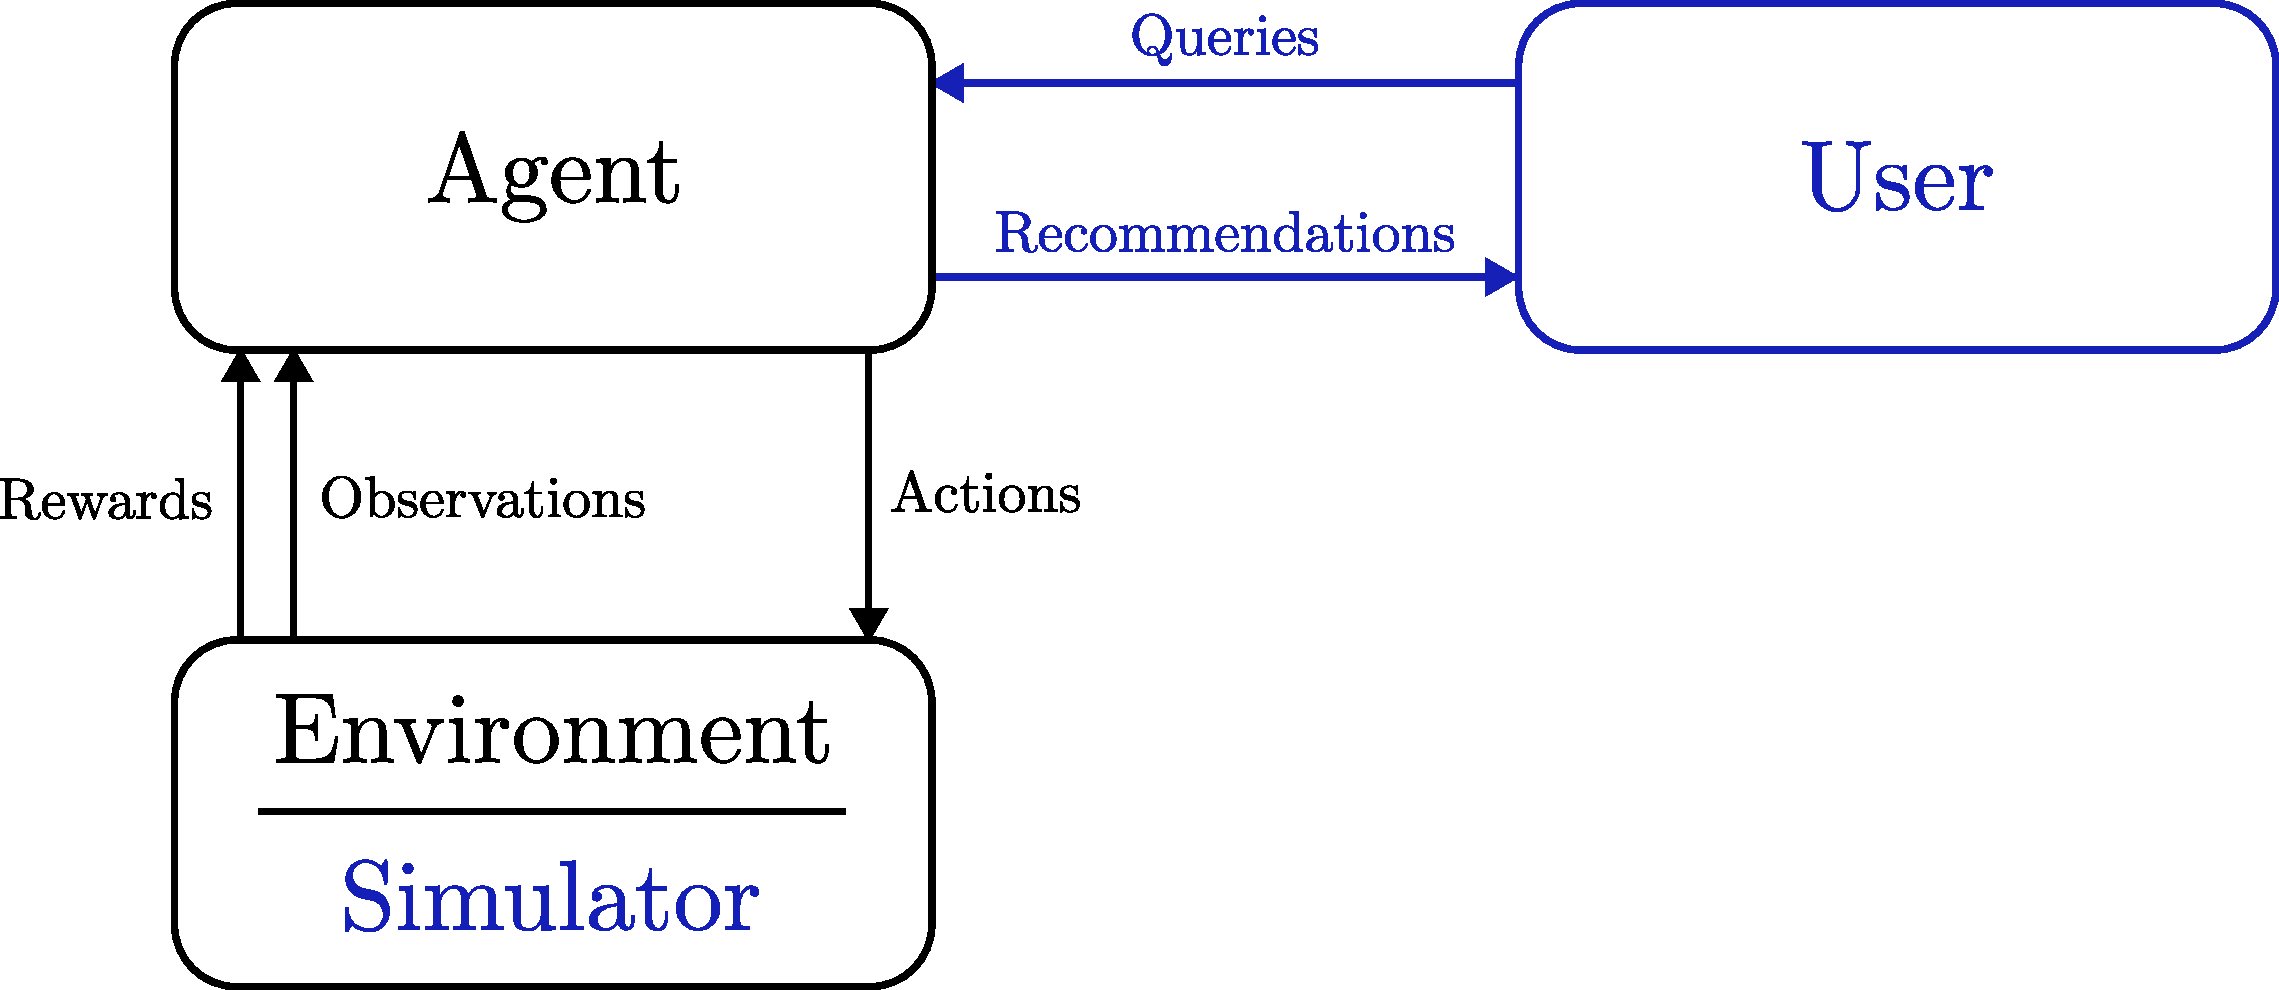
\includegraphics[width=0.75\textwidth]{figures/ch2/rl_overview.pdf} 
        \caption[Exploration setting in reinforcement learning.]{\todo{update fig to just be the blue version.} Exploration setting in reinforcement learning (\todo{reproduced and edited from fig 2.5}), \bd{where the agent aims to discover the optimal policy and has a larger emphasis on exploration to find better solutions rather than exploiting.} \todo{Cut this from main text: where the agent is only assessed on the recommendations that it provides, and is not penalised for considering poor actions in the simulator. }}
        \label{fig:4:rl_overview}
    \end{figure}
    
    Entropy is widely used in the reinforcement learning literature, commonly introduced to promote exploration and discourage convergence to suboptimal deterministic policies \cite{ppo,deep_energy_policies,a3c,reinforce_ment}. MENTS (Section \ref{sec:2-4-3-ments}), RENTS and TENTS (Section \ref{sec:3-3-3-rents-some-tents}) are all MCTS algoritms that optimise for maximum entropy objectives. While RENTS and TENTS will be considered as baselines in empirical experiments, MENTS will be used to facilitate and provide discussion around the use of entropy and maximum entropy objective.

    Section \ref{sec:4-1-intro} discusses limitations of existing MCTS algorithms in the exploration setting, motivating the work covered in the remainder of the chapter. Additionally, the planning framework is formally defined so that the algorithms can be theoretically analysed using \textit{simple regret}.
    
    In Section \ref{sec:4-2-boltzmannsearch} the \textit{Boltzmann Tree Search} (BTS) and \textit{Decaying ENtropy Tree Search} (DENTS) algorithms are defined. Section \ref{sec:4-2-3-stoch_search_policies} additionally discusses some useful properties of using a stochastic search policy in MCTS, such as naturally including prior knowledge through mixed policies, and how the Alias method (Section \ref{sec:2-6-sampling}) can be used to improve on computational complexity to answer \complexityq.

    Section \ref{sec:4-3-toyenvs} considers some theoretical MDPs, which are used to empirically demonstrate the limitations of the existing MCTS algorithms, and are additionally used to provide discussion around \entropyq.

    Results on grid world environments and the game of Go are given in section \ref{sec:4-4-results}. 

    Finally, in Section \ref{sec:4-5-theory} the main theoretical analysis and proofs are given. Convergence properties of MENTS, BTS and DENTS are proven to answer \entropyq.

    \todo{After finished writing, do another pass through neurips paper and check no results/writing missing from thesis that really should be included. (Thinking about some of the frozen lake plots in the appendix when writing this.)}
    







\section{Introduction and Motivation}
\label{sec:4-1-intro}

    In this section a grid world shortest path problem will be used to discuss the behaviour of UCT and MENTS in the exploration setting, and highlight some limitations of these algorithms. In this grid world the agent may move deterministically in any cardinal direction, North/East/South/West, provided it stays on the grid. The agent starts at the origin $(0,0)$ and the goal is to reach the other side of the grid, at $(G,G)$, where $G$ is the grid size. The cost of a path is equal to its length, and an optimal policy will always select actions that move the agent \texttt{UP} or \texttt{RIGHT}. 

    This MDPs can be defined formally:
    \begin{align}
        \cl{S} &= \{(x,y)\in\bb{N}^2 | x,y \in [0,G]\} \\
        s_0 &= (0,0) \\
        \cl{G} &= \{(x,y) \in \cl{S} | (x,y) = (G,G)\} \\
        \cl{A} &= \{(1,0),(0,-1),(-1,0),(0,1)\} = {\texttt{UP},\texttt{LEFT},\texttt{DOWN},\texttt{RIGHT}} \\
        \text{clip}((x,y)) &= \left(\max(\min(x,G),0), \max(\min(y,G),0)\right) \\
        p(s'|s,a) &= \begin{cases}
            \one[s'=s] & \text{if } s\in\cl{G} \\
            \one[s'=\text{clip}(s+a)] & \text{otherwise}
        \end{cases} \\
        H &= 6G \\
        R(s,a) &= -1 
    \end{align}

    In Section \ref{sec:4-4-results} similar grid world problems will be considered with greater complexities, such as sparse rewards and stochastic transition distributions.

    \todo{deifine sec41state consistently with diagram} \newcommand{\secfouronestate}{s^{(2,2)}}.
    
    \begin{figure}
        \centering
        \begin{subfigure}[b]{0.32\textwidth}
            \centering
            
\includegraphics[width=\textwidth]{figures/todo.jpg}
            \caption{The grid world shortest path problem.}
            \label{fig:4:shortest_path_intro_a}
        \end{subfigure}
        \hfill
        \begin{subfigure}[b]{0.32\textwidth}
            \centering
            
\includegraphics[width=\textwidth]{figures/todo.jpg}
            \caption{Red: an optimal path in shortest path problem. Green: a path that takes an optimal action \texttt{UP} at state $\secfouronestate$ but is longer than the blue path. Blue: a suboptimal path that takes one suboptimal action, \texttt{DOWN}, at state $\secfouronestate$.}
            \label{fig:4:shortest_path_intro_b}
        \end{subfigure}
        \hfill
        \begin{subfigure}[b]{0.32\textwidth}
            \centering
            
\includegraphics[width=\textwidth]{figures/todo.jpg}
            \caption{The grid world shortest path problem with the optimal soft policy for varying values of $\alphaments$, where the size of arrows indicate the probability of taking that action. Red: for a small value of $\alphaments$ the optimal actions \texttt{UP} and \texttt{RIGHT} have a much larger probability of being selected. (Roughly $\alpha \in $) \todo{add interval from results}. Green: the suboptimal actions have a significant probability of being selected, meaning that optimal paths are unlikely to be followed in a trial of MENTS. (Roughly$\alpha \in $) \todo{add interval from results}. Blue: when the temperature is sufficiently high MENTS can obtain more entropy reward each step by following a uniformly random policy. Purple: when the temperature is sufficiently high, the optimal policy for a state next to the goal is to move away from the goal so that more entropy reward can be obtained.}
            \label{fig:4:shortest_path_intro_c}
        \end{subfigure}
        \caption[An example grid world shortest path problem.]{An example grid world shortest path problem. (a) shows the grid world, (b) shows paths explored in UCT to demonstrate how it can get stuck in suboptimal solutions, and, (c) shows approximately the optimal soft policy for varying values of $\alphaments$.}
        \label{fig:4:shortest_path_intro}
    \end{figure}
    
    \begin{figure}
        \centering
        
\includegraphics[width=\textwidth]{figures/todo.jpg}
        \caption[Results on the example grid world problem for a variety of UCT bias and temperature parameters.]{Results on the example grid world problem for a variety of UCT bias and temperature parameters. \todo{Describe results}. For comparison, the Boltzmann Tree Search (BTS) and Decaying ENtropy Tree Search (DENTS) algorithms defined in Section \ref{sec:4-2-boltzmannsearch} are also shown.}
        \label{fig:4:shortest_path_intro_results}
    \end{figure}


    \subsection{UCT}

        The UCT algorithm (Section \ref{sec:2-4-2-uct}) is designed in the traditional reinforcement learning setting described in Section \ref{sec:2-3-rl}, where the UCT agent aims to minimise the cumulative regret. Thus UCT makes a trade off between exploration and exploitation during it trials, and as such will frequently choose the same action to exploit, which can result in it getting stuck in local optima when rewards are sparse or not informative. 

        A sparse reward is where the reward signal is infrequent, that is, most actions give a reward of zero. In the shortest path example, the reward is dense but relatively uninformative, as the immediate cost of taking any action is the same. 

        In Figure \ref{fig:4:shortest_path_intro_b} the shortest path problem is depicted, with an optimal path shown in red, and two paths that UCT may have explored in blue and green. When UCT is selecting an action to take from state $\secfouronestate$, it will consider the value estimates $\Quct(\secfouronestate,\texttt{DOWN})\approx $ \todo{correct number from fig} and $ \Quct(\secfouronestate,\texttt{UP})\approx $ \todo{correct number from fig}. As the Q-value estimate for taking \texttt{DOWN} is higher, UCT will most frequently select this action from state $\secfouronestate$. \todo{Some comment on how exploiting in deterministic MDP is pointlsess, and just explores same suboptimal solution over and over?}

        It is worth noting that UCT will select every action infinitely often ($N(s,a)\rightarrow \infty$ for all $s,a$) and in theory will eventually converge to the optimal policy. However, in practise this could take a long time. In Section \ref{sec:4-3-toyenvs} a theoretical MDP is considered \bd{where UCT requires a hyperexponential amount of time to find the optimal policy.}

        In Figure \todo{ref} the performance of UCT after \todo{5000} trials is given for a range of values of the UCT bias parameter $\buct$. This bias parameter controls the amount of exploration that UCT performs, and as the bias parameter is increased UCT will explore more. It can be seen that for low values of the bias parameter UCT is stuck in a suboptimal solution. When the bias parameter is increased UCT sufficiently explores to find the optimal policy. Finally, as UCT uses sample averages, for a very large bias parameter, \todo{5000} trials is not sufficient enough for $\frac{N(s,a)}{N(s)}$ \bd{to converge to a converge to a one hot distribuion}. Note that the (Q-)values of UCT can also be written as:
        \begin{align}
            \Vuct(s) &= \sum_{a \in \cl{A}} \frac{N(s,a)}{N(s)}\Quct(s,a).
        \end{align} 
        
        \todo{This issue can be resolved by taking a maximum over the Q-value estimates instead, called MaxUCT} \todo{cite}. \todo{MaxUCT will also be considered in the Section} \ref{sec:4-4-results}.


    
    
    \subsection{MENTS}
        \todo{Add somewhere in this paragraph that the temperature for which the objectives are aligned will depend on the MDP, and so when using max entropy objective, the temperature parameter will generally need to be tuned for each environment.}    

        One can argue that when using the maximum entropy objective, it is possible to recover the standard objective by setting the temperature parameter to zero, or an infitesimally small value. \todo{Add ref to energy based policies?} However, in practise, setting $\alpha$ to a tiny value will nullify the exploration advantages of using entropy. Considering the other extreme, when a very large temperature is used, entropy becomes the dominant objective in the maximum entropy objective, and the optimal soft policy will be (almost) uniform. 

        The optimal soft policy for a large temperature may be very different to the optimal policy for the standard objective. In cases such as this, it can be said that the maximum entropy objective is \textit{misaligned} with the standard objective. More precisely, the maximum entropy objective is misaligned when the policy $\pi^*_{\sft,\text{eval}}(s) = \argmax_{a'} \pi^*_{\sft}(a'|s)$ that would be followed at test time differs from the optimal standard policy $\pi^*(s)$.
        
        For a more concrete example of this phenominon, consider the shortest path example and what the optimal soft policy look like at a state next to the goal? The agent can either reach the goal in the next step, or, alternatively move away from the goal so that it can collect more entropy reward. This is depicted in Figure \ref{fig:4:shortest_path_intro_c} in purple.   

        Hence, when using the maximum entropy objective the temperature parameter often needs to be carefully tuned. Using too small of a value will nullify the exploration benefits, and using too large of a value will result in the maximum entropy objective being misaligned with the standard objective. In Section \ref{sec:4-3-toyenvs} a theoretical MDP is considered where the temperature parameter needs to be made prohibitively small to avoid the maximum entropy objective from being misaligned. 

        In Figure \todo{ref} the performance of MENTS after \todo{5000} trials is given for a range of values of the temperature parameter $\alphaments$. For temperature values up to a value of 1, a close to optimal path is found in the shortest path problem. In the range of temperatures between 1 and 100, it becomes more beneficial for MENTS to act randomly to obtain entropy but will still tend to move towards the goal, and beyond a value of 100 it becomes much more valueable to act randomly and optimise for entropy. 

        Building off this intuition, a theoretical MDP will be constructed in Section \ref{sec:4-3-toyenvs} where MENTS will either suffer from the issue of the entropy objective misalignment, or the temperature must be set to a small value that does not effectively utilise the entropy exploration. 
        
        While only the MENTS algorithm has been discussed in this section, the issue arises from mixing entropy into the scalar objective. Similar issues still arise no matter the form of entropy considered.



    \subsection{Simple Regret and Consistency}

        \todo{Move to chapter 2?}

        Now \textit{simple regret} is defined, which will be used motivate and analyse the algorithms developed. The simple regret of a policy is the difference between the value of the policy and optimal value of the policy (Equation (\ref{eq:4:simple_regret})). By definition, the optimal policy achieves a simple regret of zero, and an MCTS algorithm is considered \textit{consistent} if it's expected simple regret tends to zero. In plain english, an algorithm is consistent if left to run forever it would eventually output an optimal policy. An implication of consistency is that if an algorithm can be run for longer, then it is expected to improve on its solution.

        While \textit{cumulative regret} \todo{ref} has been used to motivate and analyse algorithms such as UCT, it is not the most appropriate measure for the exploration setting. In the exploration setting, the agent is only assessed on the recommendations it makes, and is not penalised for considering poor actions in the simulator. See Figure \ref{fig:4:planning_problem} for the formal setup of the exploring planning problem for MDPs. As such, the focus of this chapter will be on the (expected) simple regret of the algorithms developed.

        % \todo{Talk about the setup we're using. Probably want to try motive similarly to DENTS paper, and recall the diagram from} \ref{sec:2-3-rl}. \todo{Say that in fig below that normally step 3 is not considered} \todo{Neurips paper says: ``In this work, we consider scenarios where MCTS methods are used with a simulator to plan how an
        % agent should act'' in intro, and ``UCB [1] is frequently used in MCTS methods to minimise cumulative regret during the tree search.
        % Cumulative regret is most appropriate in scenarios where the actions taken during tree search have an
        % associated real-world cost. However, MCTS methods often use a simulator during the tree search,
        % where the only significant real-world cost is associated with taking the recommended action after the
        % tree search. In such scenarios, simple regret [7, 8] is more appropriate for analysing the performance
        % of algorithms, as it only considers the cost of the actions that are actually executed. Under simple
        % regret, algorithms are not penalised for under-exploiting during the search, thus can explore more,
        % which leads to better recommendations by allowing algorithms to confirm that bad actions are indeed
        % of lower value.'' in the simple regret section} 

        \begin{figure}
            \begin{tcolorbox}
                Parameters: An MDP $\cl{M}$.
                \begin{itemize}
                    \item For each round $m=1,2,...$:
                    \begin{enumerate}
                        \item the agent produces a search policy $\pi^m$ to follow;
                        \item the environment samples a trajectory $\tau\sim\pi^m$ (including rewards $r_t=R(s_t,a_t)$ for each $s_t,a_t$ pair in $\tau$);
                        \item the agent produces a recommendation policy $\psi^m$;
                        \item if the environment sends a stop signal, then the game ends, otherwise the next round starts.
                    \end{enumerate} 
                \end{itemize}
            \end{tcolorbox}
            \caption[The procedure of an exploring planning problem for MDPs]{The procedure of an exploring planning problem for MDPs, where $\psi^m$ is the recommendation policy the agent produces after $m$ trajectories are sampled using the exploration policy $\pi^m$.}
            \label{fig:4:planning_problem}
        \end{figure}

        \begin{defn}
            The \textnormal{simple regret} of a policy $\psi$ at state $s\in\cl{S}$ is the difference between the value of the policy and the optimal value at that state:
            \begin{align}
                \sreg(s,\psi) = V^*(s)-V^{\psi}(s). \label{eq:4:simple_regret}
            \end{align}
        \end{defn}

        Note that the simple regret is a random variable, as it depends on the recommendation policy $\psi$, which itself depends on the random trajectories that are sampled. Hence the expected simple regret will be the main value of interest in the theoretical analysis of Section \ref{sec:4-5-theory}.

        Now that simple regret has been defined, the concept of consistency can be defined formally:

        \begin{defn}
            An agent, that produces recommendation policies $\psi^1,\psi^2,...$ is said to be \textit{consistent} if $\bb{E}[\sreg(s,\psi^m)] \rightarrow 0$ as $m\rightarrow \infty$.
        \end{defn}
        An agent, that produces recommendation policies $\psi^1,\psi^2,...$ is said to be \textit{consistent} if $\bb{E}[\sreg(s,\psi^m)] \rightarrow 0$ as $m\rightarrow \infty$.

        Returning to the discussion around UCT and MENTS, now that simple regret and consistency have been defined, it can be shown the UCT is always consistent \todo{ref?}, whereas MENTS is only consistent for a sufficiently small temperature parameter that depends on the MDP (Section \ref{sec:4-3-toyenvs} \todo{or theory section?}). Although UCT is consistent, it can take a long time to converge to the optimal policy (as will be seen in \ref{sec:4-3-toyenvs}), and so it is of interest to develop algorithms that can explore more that are also consistent.
    










\section{Boltzmann Search}
\label{sec:4-2-boltzmannsearch}

    \todo{list}
    \begin{itemize}
        \item Recall MENTS
        \item Define BTS using THTS functions
        \item Define DENTS using THTS functions
        \item Discuss alias method variant (and complexity analysis) in a subsection?
    \end{itemize}

    \htodo{would like to read more about the exp3 stuff before submitting this ch}
    \htodo{https://tor-lattimore.com/downloads/book/book.pdf - bandits book}
    \htodo{exp3 paper: http://rob.schapire.net/papers/AuerCeFrSc01.pdf}
    \htodo{add to future work ideas to adapt BTS to use exp3 type stuff, and the thing gradient update covered in the Sutton and Barto book (todo get link and page ref to RL book where talk about that)}
    \htodo{moved already}






    \todo{Double check appendix B coverered properly here}

    \todo{Double check appendix C coverered properly here (some disucssion around when to use different algorithms and multithreading in MCTS)}

    \todo{Talk about conditions for search policy to also converge to optimal policy, and when/why that would be useful. For example, guaranteing that deeper parts of the environment are explored further. Should use this as a highlight of why UCT can be so successful, because if informative and dense reward, then you want the search policy to be exploiting, so that deeper parts of the env can be explored}





    This section defines two algorithms Boltzmann Tree Search and Decaying ENtropy Tree Search in the \thtspp\ewe schema. 




    \todo{Below is originally from sect 4.1, but better here now to tie them up}

    From the discussion in this section, the following properties are desired from the MCTS algorithms:
    \begin{itemize}
        \item define algorithms that are as simple to implement as UCT and MENTS;
        \item able to utilise dense and informative rewards (UCT \tick, MENTS \tick);
        \item effectively explore when rewards are sparse, or have sparse components (UCT \cross, MENTS \tick);
        \item are consistent, for parameters independent of the environment (UCT \tick, MENTS \cross). \todo{something like can get a reasonable result without haveing to tune params on each env. Maybe ``doesnt require parameter tuning on every environment''}
    \end{itemize}

    As such, this chapter will consider how entropy can be used as an additional secondary objective, while still focusing on performing well in the standard objective. \todo{place this better. Want it to say, that because the issue lies in the maximum entropy objective, we're going to start by stipping MENTS of the maximum entropy objective and then consider how it can be reintroduced in a consistent way.}
    
    \subsection{Boltzmann Tree Search}
    \label{sec:4-2-1-bts}

        \todo{define BTS in thtspp}

        \todo{Define with variable alpha, change proofs to say for fixed alpha get regret bound. And add theorem that }


        Our first approach, put simply, replaces the use of soft values in MENTS with 
        % \textit{dynamic programming} (DP) 
        \textit{Bellman} 
        values. We call this algorithm \textit{Boltzmann Tree Search} (BTS).  The search policy $\pi_{\textnormal{BTS}}$ and backups for the $n$th trial are given by:
        %


        This section introduces the \textit{Boltzmann Tree Search} (BTS) algorithm, presented in terms of the \thtspp\ewe schema \todo{ref}. BTS promotes exploration through the stochastic Boltzmann search policy, like MENTS \todo{ref}, while using backups that optimise for the standard objective, like UCT \todo{ref}. Unlike MENTS, the temperature parameter generalised to a function $\alphabts(x) > 0$, which allows the temperature to vary with the number of times that a node has visited. BTS uses Bellman value estimates at each node $\Vbts$ and $\Qbts$. The search policy is defined by:
        %
        \begin{align}
            \pibts(a|s) &= (1-\lambdabts)\rhobts(a|s) + \frac{\lambdabts}{|\cl{A}|}, 
                        \label{eq:4:bts_search_policy} \\ 
            \rhobts(a|s) &\propto \exp\left(\frac{1}{\alphabts(N(s))}\left(\Qbts(s,a)\right)\right).
                        \label{eq:4:bts_value_policy} \\
            \lambda(s,x) &= \min\left(1, \frac{x}{\log(e+N(s))}\right) \label{eq:4:lambda}
        \end{align}
        %
        where $\epsbts \in (0,\infty)$ is an exploration parameter and $\alphabts(x)$ is the search temperature schedule. \todo{Add a comment about defining rho as taking the max when N(s) is zero?} And given a trajectory $\tau=(s_0,a_0,r_0,...,s_{h-1},a_{h-1},r_{h-1},s_h)$ the value estimates are updated for $t=h-1,...,0$:
        \begin{align}
            \Qbts(s_t,a_t) &\leftarrow 
                R(s_t,a_t) + \sum_{s' \in \suc{s_t}{a_t}} \left( \frac{N(s')}{N(s_t,a_t)} \Vbts(s') \right), 
                        \label{eq:4:bts_backup_q} \\ 
            \Vbts(s_t) &\leftarrow \max_{a\in\cl{A}} \Qbts(s_t,a).
                        \label{eq:4:bts_backup_v} 
        \end{align}
        
        In line with the \thtspp\ewe schema, the values of $\hat{V}_{\bts}(s)$ and $\hat{Q}_{\bts}(s,a)$ are initialised using the arbitrary functions $\Vinit$ and $\Qinit$, which for example can be set to a constant value or be the output from a neural network. \todo{check all of the above definition is in line with thtspp definition} 
        
        
        When BTS needs to recommend a policy, it can use it's Q-value estimates:
        %
        \begin{align}
            \psibts(s)=\argmax_{a\in\cl{A}}\Qbts(s,a).
        \end{align}
        %
        Alternatively, the node visit counts can be used in the recommendation policy
        \begin{align}
            \mvbts(s) = \argmax_{a\in\cl{A}} N(s,a).
        \end{align}
        %
        \todo{Find better notation for this?}

        As BTS uses Bellman backups, it can be guaranteed that the BTS recommendation policy converges to the optimal standard policy. \todo{make this sound better given we're also talking about most visited recommendation policy now.}
        








        \todo{Work out how best to add the AR-BTS stuff?}

        Additionally, this search policy can still be used with average returns. The following is a summary of the definitions for \textit{Boltzmann Tree Search with Average Returns} (AR-BTS), which uses the value estimates of $\Varbts$ and $\Qarbts$ at each node, and temperature schedule $\alphaarbts(x) > 0$:
        %
        \begin{align}
            \piarbts(a|s) &= (1-\lambdaarbts)\rhoarbts(a|s) + \frac{\lambdaarbts}{|\cl{A}|}, 
                        \label{eq:arbts_search_policy} \\ 
            \rhobts(a|s) &\propto \exp\left(\frac{1}{\alphaarbts(N(s))}\left(\Qarbts(s,a)\right)\right).
                        \label{eq:arbts_value_policy}
        \end{align}
        %
        where $\epsarbts \in (0,\infty)$ is an exploration parameter and $\alphaarbts(x)$ is the search temperature schedule. Given a trajectory $\tau=(s_0,a_0,r_0,...,s_{h-1},a_{h-1},r_{h-1},s_h)$ and the leaf node value estimate $\tilde{r} = \Vinit(s_h)$, the value estimates are updated for $t=h-1,...,0$:
        \begin{align}
            \Qarbts(s_t,a_t) &\leftarrow 
                \frac{1}{N(s_t,a_t)} \left( (N(s_t,a_t)-1) \Qarbts(s_t,a_t) 
                    + \tilde{r} + \sum_{i=t}^{h-1} r_i \right) \label{eq:4:arbsts_backup_q} \\
            \Varbts(s_t) &\leftarrow 
                \frac{1}{N(s_t)} \left( (N(s_t)-1) \Varbts(s_t) 
                    + \tilde{r} + \sum_{i=t}^{h-1} r_i \right). \label{eq:4:arbsts_backup_v} 
        \end{align}

        Similarly to BTS, either the Q-value estimates can be used for a recommendation policy or the most visited child node can be used:
        \begin{align}
            \psiarbts(s) &= \argmax_{a\in\cl{A}}\Qbts(s,a), \\
            \mvarbts(s) &= \argmax_{a\in\cl{A}} N(s,a).
        \end{align}
        %
        \todo{Still find better notation for this?}








        In Section \todo{ref} convergence results about BTS and AR-BTS are given, which are summarised below:
        %
        \begin{itemize}
            \item BTS is consistent and converges for any setting of parameters;
            \item if $\alphabts(x) \geq L > 0$: BTS converges with an theoretical exponential rate;
            % \item if $\alphabts(x) \rightarrow 0$: BTS converges still;
            \item $\alphaarbts(x) \rightarrow 0$: AR-BTS converges;
        \end{itemize}
        %
        noting that these results are independent of all of the other parameters, including which of the two recommendation policies are used. \todo{didnt bother with exponential convergence rate for most visited, and not 100 percent its true, but think it should be}

        \todo{Add theorems here? Or just reference theorems? - later note: think summarise the properties in words, and reference the theorems in the theory section.}

        \todo{Is the upper bound needed for arbts? Revisit these after having written the proofs up.}








        % By using Bellman backups, we can guarantee that the BTS recommendation policy converges to the optimal standard policy for any temperature $\alpha$, given enough time. In other words, BTS is consistent.
        % %
        % \begin{theorem} 
        %     \label{thrm:bts}
        %     For any MDP $\cl{M}$, after running $n$ trials of the BTS algorithm with a root node of $s_0$, there exists constants $C,k>0$ such that for all $\varepsilon>0$ we have $\bb{E}[\sreg(s_0,\psibts)] \leq C\exp(-kn)$, and also $\Vbts(s_0) \rap V^*(s_0)$ as $n\rightarrow\infty$.
        % \end{theorem}

        % \todo{update for $\alpha$ being const etc. Add the more theorems about BTS here.}
        % \begin{proofoutline}
        % 		This result is a special case of Theorem \ref{thrm:dents} by setting $\beta(m)=0$.
        % \end{proofoutline}
        % \begin{proof}
        %     Proofs for Theorem \ref{thrm:bts} and Theorem \ref{thrm:dents} provided in Appendix \ref{app:proofs}.
        % \end{proof}






    
    \subsection{Decaying ENtropy Tree Search}
    \label{sec:4-2-2-dents}

        \todo{add label}
        \todo{define DENTS in thtspp}

        \textit{Decaying ENtropy Tree Search} (DENTS) extends the BTS algorithm by introducing \textit{entropy estimates}. In DENTS nodes have a secondary entropy value estimate, $\HVdents$ and $\HQdents$, which are monte carlo estimates the entropy of the search policy rooted from the relevant node. By keeping a separate estimate for entropy, DENTS is able to use entropy in it's search policy, and discard it for recommendations.

        Given a trajectory $\tau=(s_0,a_0,r_0,...,s_{h-1},a_{h-1},r_{h-1},s_h)$, the entropy values are updated as follows for $t=h-1,...,0$:
        \begin{align}
            \HVdents(s_t) &\leftarrow \cl{H}(\pidents(\cdot | s_t)) + \sum_{a\in\cl{A}} \pidents(a|s_t)\HQdents(s_t,a), 
            \label{eq:4:dents_entropy_v_backup} \\
            \HQdents(s_t,a_t) &\leftarrow \sum_{s'\in \suc{s_t}{a_t}} \frac{N(s')}{N(s_t,a_t)} \HVdents(s'), 
            \label{eq::4dents_entropy_q_backup}
        \end{align}
        %
        where $\cl{H}$ is the Shannon entropy function. \todo{sentence about how the entropy values are initialised} $\HVdents(s) \leftarrow 0$.

        The entropy values are used as an exploration bonus in the search policy, and are weighted by a non-negative function $\betadents(x)\geq 0$. Generally this will be set to a function such that $\betadents(x)\rightarrow 0$ as $x\rightarrow\infty$ and will achieve better theoretical performance in this case. The DENTS search policy $\pidents$ is defined follows:
        %
        \begin{align}
            \pidents(a|s) &= (1-\lambdadents)\rhodents(a|s) + \frac{\lambdadents}{|\cl{A}|}, 
                        \label{eq:dents_search_policy} \\ 
            \rhodents(a|s) &\propto \exp\left(\frac{1}{\alphadents(N(s))}\left(\Qdents(s,a)+\beta(N(s))\HQdents(s,a)\right)\right).
                        \label{eq:dents_value_policy}
        \end{align}

        And finally, given the the trajectory $\tau$ the Bellman value estimates for DENTS, $\Vdents$ and $\Qdents$ are updated identically to BTS for $t=h-1,...,0$:
        \begin{align}
            \Qdents(s_t,a_t) &\leftarrow 
                R(s_t,a_t) + \sum_{s' \in \suc{s_t}{a_t}} \left( \frac{N(s')}{N(s_t,a_t)} \Vbts(s) \right), 
                        \label{eq:dents_q_backup} \\ 
            \Vdents(s_t) &\leftarrow \max_{a\in\cl{A}} \Qbts(s_t,a), 
                        \label{eq:dents_v_backup} 
        \end{align}

        \todo{also give the recommendation policies}

        




        \todo{Write about AR-DENTS here? My brain is getting bored copying and slightly editing things. this is just copying dents and then copying the value backups from ar-bts}






        Section \todo{ref} also provides convergence results about DENTS and AR-DENTS are given, which are summarised below:
        %
        \begin{itemize}
            \item When using the \todo{default? Bellman?} recommendation policy:
            \begin{itemize}
                \item DENTS is consistent and converges for any setting of parameters;
                \item if $\alphadents(x) \geq L > 0$: DENTS converges with an theoretical exponential rate;
                \item if $\alphaardents(x) \rightarrow 0$ and $\frac{\betaardents(x)}{\alphaardents(x)} \rightarrow 0$: AR-DENTS converges;
            \end{itemize}
            \item When using the most visited recommendation policy, the same results hold, but additionally requires $\frac{\betaardents(x)}{\alphaardents(x)} \rightarrow 0$ if it was not already a requirement. \todo{didnt bother with exponential convergence rate for most visited, and not 100 percent its true, but think it should be}
        \end{itemize}

        \todo{Add theorems here? Or just reference theorems? - later note: think summarise the properties in words, and reference the theorems in the theory section.}

        \todo{Double check these after having written up the proofs. Particularly the differences between using the two different recommendation policies.}









    \subsection{Advantages of Stochastic Search Policies}
    \label{sec:4-2-3-stoch_search_policies}

        Using a stochastic search policy in MCTS (or \thtspp) provides more benefits than just encouraging exploration through randomly sampled actions. In particular, the Alias Method (Section \ref{sec:2-6-sampling}) can be used to trade off using the most up to date policy for computational speed. Moreover, when prior knowledge (in the form of a policy prior) is available \todo{cite alphago etc}, it can naturally be integrated into the search using a \textit{mixture policy}.

        \todo{add ref to} \complexityq






        \subsubsection{The Alias Method in MCTS}

        \todo{Double check appendix C coverered properly here (complexity stuff here)}

        When using the Alias Method in \thtspp\ewe an alias table \todo{capitalise?} is constructed at every decision node. This table can be updated every $\lambda|\cl{A}|$ visits to the node, for an arbitrary $\lambda\in\bb{R}_{>0}$, giving an amortised complexity of $O(1)$. \todo{just say constant amortised complexity?} $O(O(1)+\frac{|\cl{A}}{\lambda|\cl{A}|}) = O(O(1)+\frac{1}{\lambda}) = O(1)$. \todo{probably dont need to do that maths.} In \thtspp the value of the $\lambda$ can be varied to adjust the trade off between The value of lambda can be varied to adjust the trade off between up-to-dateness and sampling speed. For the remainder \todo{find a better way of saying this}, $\lambda=1$ will be considered \todo{but all of the results still hold}. Note that when a new decision node is constructed and added to the tree, there will still be a cost of $O(|\cl{A}|)$ to construct the new alias table.
        
        Although this will always lead to quite a significant computational speedup, in the case where \mctsmode, the computational speedup is also asymptotic. \todo{where this paragraph go?}

        In the following, the computational complexity to run $n$ trials is considered.
        
        First consider the computational complexity of running UCT: at each decision node visited on a trial, the maximum over $|\cl{A}|$ values is computed \todo{this is worded poorly}, on each trial at most $H_{\thtspp}$ decision nodes will be visited. Hence, the computational complexity of running $n$ trials of UCT is $O(nH_{\thtspp}|\cl{A}|)$.

        \todo{copy out appendix C stuff, cleaning up above and below as needed}

        Finally, considering the case when \thtspp\ewe is not running in \mctsmode, the asymptotic complexity is still $O(nH_{\thtspp}|\cl{A}|)$, as each trial is sampled until the planning horizon $H_{\thtspp}$ 

        \todo{Talk about co}

        \todo{add label}
        \todo{write about alias sampling}


        






        \subsubsection{Encorporating Prior Knowledge Through Mixture Policies}

        Let $\pi$ be some \thtspp\ewe search policy, and supposed that we have access to another policy $\tilde{\pi}$ with prior knowledge, such as a neural network. Then a new search policy $\pi_{\text{mix}}$ can be naturally be defined using a mixture of $\pi$ and $\tilde{\pi}$.

        \todo{some comment about just using the same mixing function as before ... because? .. it lets it tend towards the correct thing}

        The mixture policy is defined by:
        \begin{align}
            \pi_{\text{mix}}(a|s) = 
                (1-\lambda(s,\epsilon_{\text{mix}})) \pi(a|s) 
                + \lambda(s,\epsilon_{\text{mix}}) \tilde{\pi}(a|s),
        \end{align}

        where $\lambda$ is the same function as defined in equation (\todo{ref}), and $\epsilon_{\text{mix}}\in(0,\infty)$ weights the amount to use the prior knowledge by. \todo{word better}.

        \todo{are there theoretical results? Maybe we can show that for arbitrary function that it doesnt change anything. It should be the same as mixing in the uniform. Also another good reason to use the same function, because then the proof is basically the same thing as before.}


        
        \todo{write about using $\tilde{\pi}$, $\tilde{Q}$, $\tilde{V}$?}
        \todo{talk about grid world and how Qinit need to be able to handle costs}

        \todo{discuss the MENTS intiialisation here? :} MENTS suggests using $\tilde{\pi}$ as \todo{their description, find where we talked about it in neurips. ACTUALLY, this should be in the ments section and reffed from here}
        %
        However, this may still lead to issues in for example in grid world problems. \todo{talk about how log probs are negative, so although init policy is correct on first visit, could to more damage than benefit. Also this should be either in ch2 or ch3 too?}




        \todo{<beg> is original writing on encorporating prior knowledge from neurips}
        This section describes how to use value and policy networks in BTS. Adapting MENTS and DENTS are similar (Appendix \ref{app:adapt_for_nets}). Values can be initialised with the neural networks as $\hat{Q}(s,a)\leftarrow\log \tilde{\pi}(a|s)+B$ and $\hat{V}(s)\leftarrow\tilde{V}(s)$, where $B$ is a constant (adapted from Xiao \etal \todo{cite}%\cite{xiao2019maximum})
        . With such an initialisation, the initial BTS policy is 
        $\rho_{\textnormal{BTS}}(a|s)\propto\tilde{\pi}(a|s)^{1/\alpha}$. For these experiments we set a value of $B=\frac{-1}{|\mathcal{A}|}\sum_{a\in\mathcal{A}} \log\tilde{\pi}(a|s)$. Additionally, the stochastic search policy naturally lends itself to mixing in a prior policy, so we can replace BTS search policy $\pi_{\textnormal{BTS}}$ (Equation (\ref{eq:bts_search_policy})) with $\pi_{\textnormal{BTS,mix}}$:
        % 
        \begin{align}
            \pi_{\textnormal{BTS,mix}}(a|s) 
            &= \lambda_{\tilde{\pi}}\tilde{\pi}(a|s) + (1-\lambda_{\tilde{\pi}}) \pi_{\textnormal{BTS}}(a|s) \\
            &= \lambda_{\tilde{\pi}}\tilde{\pi}(a|s) + (1-\lambda_{\tilde{\pi}})(1-\lambda_s)\rho_{\textnormal{BTS}}(a|s) + \frac{(1-\lambda_{\tilde{\pi}})\lambda_s}{|\cl{A}|}, %\label{eq:ments_mixed_policy}
        \end{align}
        % 
        where $\lambda_{\tilde{\pi}}=\min(1,\epsilon_{\tilde{\pi}}/\log(e+N(s)))$, and $\epsilon_{\tilde{\pi}} \in (0,\infty)$ controls the weighting for the prior policy.
        \todo{<end> is original writing on encorporating prior knowledge from neurips}









    \subsection{Things still missing in this section}
        Defining the average reward versions of the algorithms

        \todo{Talking about the OG DENTS algorithm and why that didn't work? I feel like its a reasonable question}










\section{Toy Environments}
\label{sec:4-3-toyenvs}

    \todo{Sometimes feel like I'm bashing on MENTS. Want to make it clearer that I'm not bashing on MENTS, but using MENTS (as the max entropy MCTS method) to demonstrate issues with the max entropy objective itself.}

    This subsection uses theoretical MDPs to further highlight and discuss the benefits and pitfalls of UCT and MENTS, \todo{and compares the performance of BTS and DENTS on these MDPs.} 

    The \textit{D-chain problem} introduced by \todo{cite} (Figure \ref{fig:modified_d_chain}), is a deterministic MDP for which \todo{UCT ``struggles'' (find better words, maybe here say that wont feasibly solve)}. From some state $d$ if the action $a_L$ is taken the trial ends and a reward of $(D-d)/D$ is received, and from the final state in the chain, $D$, if the action $a_R$ is taken then the maximum reward of $R_f=1$ is received. Hence, the optimal standard policy will always take action $a_R$ at every state achieve a return of $1$.
    %
    \todo{Make sure that notation is consistent with the new fig}
    %
    \begin{figure}
        \centering
        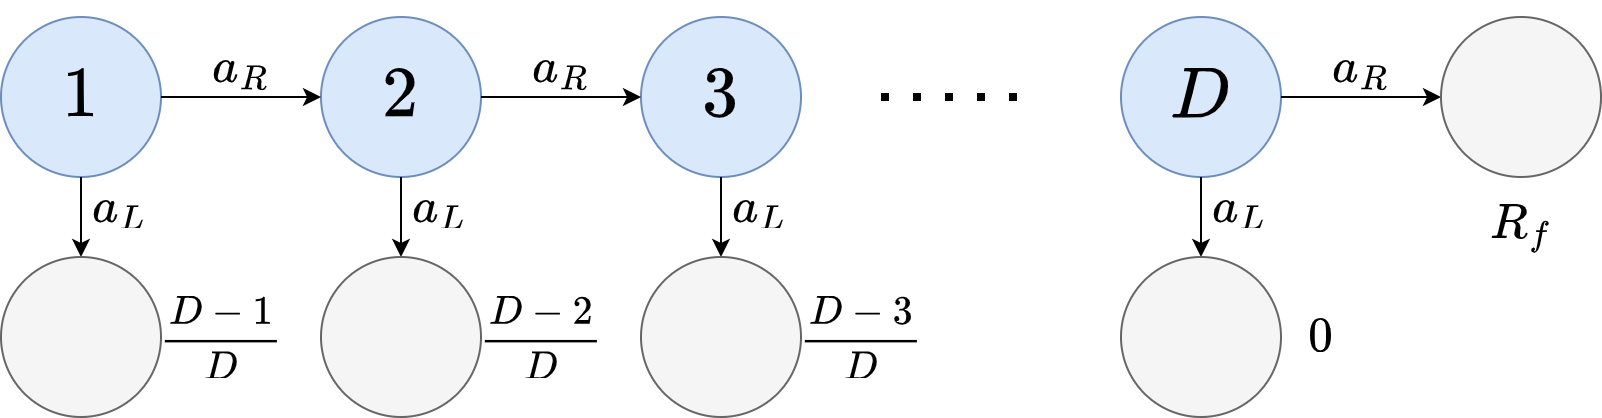
\includegraphics[width=0.6\textwidth]{figures/temp/dchain.png}
        \caption[An illustration of the \textit{(modified) D-chain problem}.]{An illustration of the \textit{(modified) D-chain problem}, \todo{where 1 is the starting state, and values next to sink states represent the reward for arriving in that state. At the end of the chain a reward of } $R_f$ \todo{ is recieved, where in} \todo{cite} the reward at the end of the chain is set to $R_f=1$. \todo{Temp fig}}
        \label{fig:modified_d_chain}
    \end{figure}

    \todo{cite} show that UCT requires $\Omega(\exp(...\exp(1)...))$ many trials (D composed exponential functions) to recommend the optimal actions $a_R$. \bd{Informally, this behaviour stems from the value estimate of state 2 remaining below D-1/D for a long time, and UCT repeatedly taking action aL on its trials once its confidence intervals become relatively concentrated. UCT will still always explore the aR action and eventually converge to the optimal value estimates (and recommendation policy), but in practise it would take longer than a human lifetime.}

    Where in Section \todo{ref} UCT can be seen to perform well in the presence of an informative dense reward, and struggle when only given an uninformative sparse reward, this MDP sets the rewards to take advantage of this \bd{behaviour maximally. The MDPs rewards can be viewed from the perspective of the dense rewards along the chain that essentially suggest ``don't explore this way'', which are hiding the sparse reward of one at the end of the chain.}

    In stark contrast, when MENTS is run on the D-chain problem, it quickly explores and finds the sparse reward of one at the end of the chain. This is largely because of the maximum entropy objective, where there \bd{is no entropy reward to be gained by traversing to a sink state, thus encouraging MENTS to follow the chain}. However, because the chain is explored largely due to the maximum entropy objective, consider what happens in the \textit{modified D-chain problem}, where the reward at the end of the chain is set to $R_f=1/2$. \todo{copy out the soft Q value computations with temp of one.}

    These two cases $R_f \in {1/2,1}$ demonstrate that MENTS, and more generally whenever using the maximum entropy objective, the optimal temperature parameter to be used is dependent on the MDP, and can vary massively even with small changes in the MDP, as for example in this the value of a single reward was changed. \todo{Reference the result that for any temperature there is an MDP where MENTS will be inconsistent}

    \todo{Generally write up a bit cleaner once have plots in}

    BTS and DENTS improve on this theoretically as convergence can be guarunteed by parameter settings which are independent of the MDP. In practise, for example consider using a constant value for $\alphadents$ and $\betadents$, the search policy can behave similarly to MENTS, \bd{which could be an issue in more complex MDPs} \todo{some of this discussion more appropriate for entropy trap bit maybe?}



    \todo{plots to add: the two plots from neurips, performance of MENTS/BTS/DENTS for varying settings of temperature parameters. Same plots for entropy trap D-chain. Also demonstrate that if temperatures decayed properly then DENTS will visit the optimal sink state in entropy D-chain lots, while if not decayed, then will recommend the correct thing, but not visit. Last one is of practical importance, where the sparse reward of one at the end isn't just a sink state but the rest of the MDP where you actually want to do something important.}


    \bd{(Commented out old writing below this). It is often argued in the maximum entropy objective that the standard objective can be recovered by setting the temperature suffficiently small, however this looses the benefits of using entropy for exploration.} \todo{Ref the result about ments converging for a sufficiently small temperature here.}
    % In the maximum entropy objective, it is argued that the standard objective can be recovered by setting $\alpha=0$ or setting $\alpha$ infitesimally small ($0<\alpha<<1$). \todo{add quote}. 
    % %
    % \todo{Although this is theoretically true (TODO ref the result about MENTS), in practise it is desirable to use the largest temperature that doesn't lead to undesirable (random) behaviour. In other words, extermely small temperatures do not utilise entropy for exploration effectively, while extremely large temperatures encourage agents to act randomly rather (reword: optimise for the standard objective). MENTS is used in (TODO) to demonstrate this issue with the maximum-entropy objective empirically, and (TODO) provides a corresponding theoretical result around MENTS.}
    % %
    % Although this is true, the most benefit can be gained from using entropy as an exploration bonus by setting a larger value of $\alpha$. This is highlighted in Figure \todo{ref}, where the performance on MENTS on the modified D-chain environment can be seen to improve as $\alpha$ is made larger, until a sudden drop off when it surpasses a threshold (\todo{at the poing 0.142ish}).


    By making this observation that maximum entropy algorithms can be mislead by providing an opportunity to accrue the `entropy reward', the D-chain problem can be further adapted, such that neither UCT or MENTS will perform well for any parameter settings. To construct the \textit{D-chain with entropy trap} \bd{problem? MDP?}, the same chain of length $D$, or the \textit{UCT gauntlet}, is used from the D-chain problem, and as such UCT will also struggle on this problem. However, at the end of the chain this time, one more choice is left, to either take the immediate reward of one, or to enter the \textit{entropy trap}, which is a sequence of states with zero rewards that allows a policy to act randomly to gain an entropy reward.
    %
    \begin{figure}
        \centering
        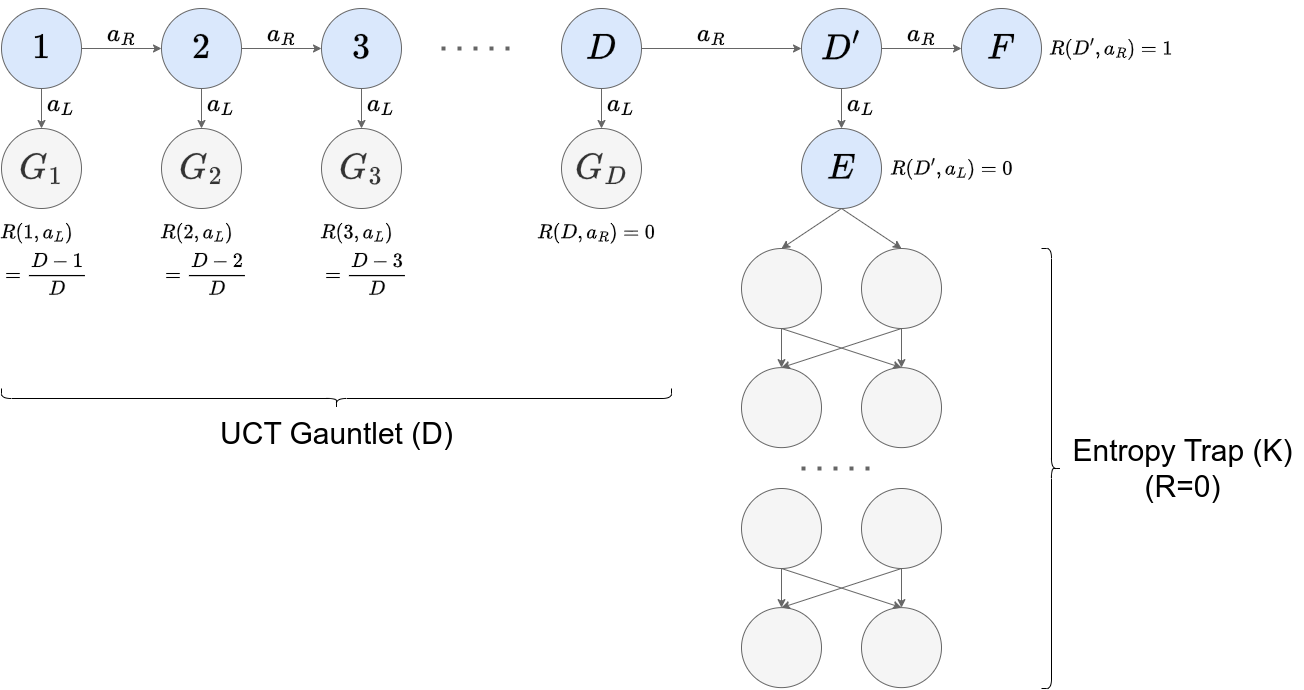
\includegraphics[width=0.6\textwidth]{figures/temp/entropy_trap.png}
        \caption[An illustration of the \textit{(modified) D-chain problem with entropy trap}.]{An illustration of the \textit{(modified) D-chain problem with entropy trap}, \todo{write caption describing MDP after made it}. \todo{Temp fig}}
        \label{fig:d_chain_entropy_trap}
    \end{figure}

    \todo{These claims made more concrete in (ref theorem)}

    \todo{Some writing about what the plots show empirically once run this.}

    \todo{Wrap up this section saying that although these are highly theoretical and constructed examples, it can help even in practise to think about these things and consider the performance on these envs to understand why these algorithms behave the way they do on real problems. For example, it may be the case that there are some subtle entropy traps, consider if instead that Rf was 10, and the entropy trap had a reward of 9 (including the entropy bit), such that the performance looked good but } \todo{Basically a bit of chatting to map back to these things in practise and why useful, maybe also add something like this at the top. Actually, add this at the top, and then point out the specifics at the end. Good sandwitch storytelling.}

    \todo{Below is parameter sensitivity section from neurips appendix D. Extract whats useful, but better results should demonstrate this better}

    We run each algorithm with a variety of $\alpha$ temperatures, and the $\epsilon$ exploration parameter on the 10-chain environments (Figure \ref{fig:dchain_illustration}). Additionally, we ran UCT with a variety of bias parameters. Figures \ref{fig:uct_10chain_hps}, \ref{fig:ments_10chain_hps}, \ref{fig:rents_10chain_hps}, \ref{fig:tents_10chain_hps}, \ref{fig:bts_10chain_hps} and \ref{fig:dents_10chain_hps} give results for the 10-chain environment, with algorithms UCT, MENTS, RENTS, TENTS, BTS and DENTS respectively. Figures \ref{fig:uct_10chain_half_hps}, \ref{fig:ments_10chain_half_hps}, \ref{fig:rents_10chain_half_hps}, \ref{fig:tents_10chain_half_hps}, \ref{fig:bts_10chain_half_hps} and \ref{fig:dents_10chain_half_hps} give results for the modified 10-chain environment, with algorithms UCT, MENTS, RENTS, TENTS, BTS and DENTS respectively. 

    As expected with UCT, regardless of how the bias parameter is set, in both the 10-chain ($D=10$, $R_f=1.0$) and modified 10-chain ($D=10$, $R_f=0.5$) environments, it only achieves a value of $0.9$. See Figures \ref{fig:uct_10chain_hps} and \ref{fig:uct_10chain_half_hps} for plots.

    As discussed in Section \ref{sec:limitations}, for higher temperatures in MENTS it will find the reward of $R_f$ in both the 10-chain and modified 10-chain environments. At a temperature of $\alpha=0.15$ MENTS is able to find the reward of $R_f=1$ on the 10-chain (Figure \ref{fig:ments_10chain_hps}), but will still recommend a policy that gives the reward of $R_f=0.5$ on the modified 10-chain (Figure \ref{fig:ments_10chain_half_hps}). At a temperature of $\alpha=0.1$ MENTS will struggle to find the reward of $R_f=1$ in the 10-chain, without the help of the exploration parameter, but this is the first temperature we tried that was able to recommend the optimal policy in the modified 10-chain (Figure \ref{fig:ments_10chain_half_hps}). For low temperatures, such as $\alpha=0.01$, MENTS was able to find the optimal policy, but in the case of the 10-chain with $R_f=1$ it can only do so with the help of a higher exploration parameter.

    When we ran TENTS on the (modified) 10-chain, we see results that parallel MENTS, see Figures \ref{fig:tents_10chain_hps} and \ref{fig:tents_10chain_half_hps}. Interestingly, RENTS was only able to find the reward of $R_f=1$ on the 10-chain environment if we used a low temperature, $\alpha=0.01$ and a high exploration parameter, $\epsilon=10$. Otherwise, RENTS tended to behave similarly to UCT on these environments, see Figures \ref{fig:rents_10chain_hps} and \ref{fig:rents_10chain_half_hps}.

    In contrast, BTS was able to find the reward of $R_f=1.0$ in the 10-chain when a high search temperature or high exploration parameter was used (Figure \ref{fig:bts_10chain_hps}). And, in the modified 10-chain, BTS always achieves a reward of $0.9$ regardless of how the parameters are set (Figure \ref{fig:bts_10chain_half_hps}). DENTS performance on the 10-chain (Figure \ref{fig:dents_10chain_hps}) and modified 10-chain (Figure \ref{fig:dents_10chain_half_hps}) was similar to BTS, but tended to find the reward of $R_f=1$ in the 10-chain marginally faster. For the decay function $\beta$ in DENTS, we always set $\beta(m)=\alpha/\log(e+m)$ for these experiments.

    To demonstrate that the $\epsilon$ exploration parameter is insufficient to make up for a low temperature, we also consider the 20-chain ($D=20$, $R_f=1$) and modified 20-chain ($D=20$, $R_f=0.5$) problems. We don't give plots for all algorithms on both of the 20-chain environments like we do for 10-chain environments, but opt for the plots that demonstrate something interesting. 
    
    In Figure \ref{fig:ments_20chain_hps} we see MENTS on the 20-chain is able to find the reward of $R_f=1$ for higher temperatures. However, this time, the exploration parameter does not make much of an impact when using lower temperatures. Moreover, a large exploration parameter appears to negatively impact MENTS ability to find $R_f=1$. This makes sense considering that a uniformly random policy will find the reward at the end of the chain once every $2^{10}$ trials in the 10-chain, but only once every $2^{20}$ in the 20-chain. Again, on the modified 20-chain, MENTS is only able to recommend the optimal policy for low temperatures (see Figure \ref{fig:ments_20chain_half_hps}). 

    When we ran BTS on the 20-chain, it was unsuccessful at finding the final reward of $R_f=1$, which makes sense as it is not using entropy for exploration, and it is unlikely to follow a random policy to the end of the chain (Figure \ref{fig:bts_20chain_hps}). For DENTS, we again used a decay function of $\beta(m)=\alpha/\log(e+m)$ for simplicity, and unfortunately it was only able to make slow progress towards finding the final reward of $R_f=1$ for high temperatures. However, if we independently set the values of $\alpha$ and 
    
    However, DENTS on the 20-chain begins to make slow progress towards finding the final reward of $R_f=1$, but requires a higher temperature to be used, as we decay the weighting of entropy over time (Figure \ref{fig:dents_20chain_hps}). Again we used a decay function of $\beta(m)=\alpha/\log(e+m)$ here for simplicity, and if we properly select them DENTS is more than capable of solving the 20-chain. For example we show that using DENTS with $\alpha=0.5$, $\beta(m)=10/\log(e+m)$ and $\epsilon=0.01$ in Figure \ref{fig:dents_20chain_tuned}, where $\alpha$ is set low enough that there is still a high probability of following the chain to the end, $\beta$ is set to be large initially to encourage exploring with the entropy reward and $\epsilon$ is set low to avoid random exploration ending trials before reaching the end of the chain. If we were to run DENTS and BTS on the modified 20-chain they would recommend the optimal policy giving a value of $0.95$ for all of the parameters we searched over (not shown).
    
    Finally, in Figure \ref{fig:dbments_20chain_hps} we also consider running DENTS, but instead setting $\beta(m)=\alpha$ to replicate MENTS. The main difference between DENTS in this case and MENTS is the recommendation policy, where DENTS uses the Bellman values for recommendations, rather than soft values. So even in cases where the MENTS search is more desirable, we can replicate it with DENTS while providing recommendations for the standard objective. Moreover, running DENTS with $\beta(m)=\alpha$ on the modified 20-chain would always yield the optimal value of $0.95$ because of the use of Bellman values for recommendations (not shown).


    \todo{A MILLION FIGURES WERE HERE}











\section{Empirical Results}
\label{sec:4-4-results}

    \htodo{SHOULD WE DO VALUE NORMALISATION IN THE AUX EXPR TOO?}
    
    \htodo{Wasn't too careful about changing from active voice to passive voice here in this entire section}

    \htodo{Get some better results using hyperparam optimise //// want a dense env where the (not entropy) temp decay fn gets optimised to soemthing that decays a lot /// want a sparse env where the temp decay fn gets optimised to something flat (or basically flat)}

    This section provides empirical results on gridworld environments and on the game of Go. It begins by describing the evaluation setup, and environments, followed by the empirical results and discussion. The main algorithms discussed in this chapter, BTS and DENTS will be evaluated, using UCT \todo{ref}, MENTS \todo{ref}, RENTS \todo{ref}, TENTS \todo{ref} and H-MCTS \todo{ref litrev}. \bd{H-MCTS is used as an UCT style MCTS algorithm that is also designed using simple regret for comparison.} 




    \subsection{Environments}

        \subsubsection{(Deterministic) Frozen Lake}
            The \emph{(Deterministic) Frozen Lake} is a grid world environment with one goal state. The agent can move in any cardinal direction at each time step, and walking into a wall leaves the agent in the same location. Trap states exist where the agent falls into a hole and the trial ends. If the agent arrives at the goal state after $t$ timesteps, then a reward of $0.99^t$ is received. \todo{this is c and p from neurips} \todo{also run with the more reasonable reward, was only doing this reward to make plots look nicer, but should just put in a bit of time to make the plots not look terrible with the more sensible reward}

            \bd{This Frozen Lake environment is used to evaluate the algorithms in a sparse reward environment}

            \todo{ TWO: would like to have experiments which vary the proportion of the sparse reward. So have FL(lambda), where lambda specifies the ratio between the dense and sparse rewards. Then investigate what happens as vary lambda. So this is the grid world experiments run again, }

            \todo{mention some of the above talked about simpler versions of this without holes.}

            \todo{Why did we keep it deterministic? Maybe do some smaller ones with transition noise?}

            \todo{Below is the frozen lake details from appendix, merge into main prose}

            For space, the specific maps for the gridworlds are omitted from the results section in the main paper. In the gridworld maps, \texttt{S} denotes the starting location of the agent, \texttt{F} denotes spaces the agent can move to, \texttt{H} denote holes that end the agents trial and \texttt{G} is the goal location. 
        
            In Figure \ref{fig:fl8} we give an 8x8 Frozen Lake environment that is used in Section \ref{app:param_sens} to demonstrate how the different algorithms perform with a variety of temperatures. Figure \ref{fig:fl12} gives the 8x12 Frozen Lake Environment that is used for hyperparameter selection in Section \ref{app:hps}. And in Figure \ref{fig:fl12test} we give the 8x12 Frozen Lake Environment that is used to test the algorithms in Section \ref{sec:results}. Each of these maps was randomly generated, with each location having a probability of $1/5$ of being a hole, and the maps were checked to have a viable path from the starting location to the goal location.
        
            \begin{figure}
                \centering
                \begin{subfigure}[b]{0.3\textwidth}
                    \centering
                    \texttt{SFFFFFHF} \\
                    \texttt{FFFFFFFF} \\
                    \texttt{FHFHFFFF} \\
                    \texttt{FFFFFFHH} \\
                    \texttt{FFFHFFFF} \\
                    \texttt{FHHHFFFF} \\
                    \texttt{FFFFFHFF} \\
                    \texttt{FFFFFFFG} 
                    \caption{8x8 Frozen Lake.}
                    \label{fig:fl8}
                \end{subfigure}
                \hfill
                \begin{subfigure}[b]{0.3\textwidth}
                    \centering
                    \texttt{SFHFFFHFFFFF} \\
                    \texttt{FFFFFFFHFFFF} \\
                    \texttt{HFFFFFHFFFFF} \\
                    \texttt{FHFFHFFFFFFF} \\
                    \texttt{HHFFFFFFFFFF} \\
                    \texttt{FHFFFFHFFFFF} \\
                    \texttt{FHFFFHHFHFFF} \\
                    \texttt{FFFFFFFFFHHG} 
                    \caption{8x12 Frozen Lake.}
                    \label{fig:fl12}
                \end{subfigure}
                \hfill
                \begin{subfigure}[b]{0.3\textwidth}
                    \centering
                    \texttt{SFHFFFFFFFHF} \\
                    \texttt{FFFFFFFFFFFF} \\
                    \texttt{FHFFFFHFFFFF} \\
                    \texttt{FFFHFFFFFFHF} \\
                    \texttt{FFFFFFFFFFFF} \\
                    \texttt{FFFFHFFFHFFF} \\
                    \texttt{FFHFFFFFFFFH} \\
                    \texttt{FFFFFFFFFFFG} 
                    \caption{8x12 Test Frozen Lake.}
                    \label{fig:fl12test}
                \end{subfigure}
                \caption{Maps used for experiments using the Frozen Lake environment in Sections \ref{sec:results}, \ref{app:param_sens} and \ref{app:hps}. \texttt{S} is the starting location for the agent, \texttt{F} represents floor that the agent can move too, \texttt{H} are holes that end the agents trial and \texttt{G} is the goal location.}
                    \label{fig:maps}
            \end{figure}

        \subsubsection{Sailing Problem}
            The \emph{Sailing Problem} is a grid world environment with one goal state, at the opposite corner to the starting location of the agent. \todo{This problem was introduced in <TODO, think ref is this commented out one> %\cite{peret2004line}   
            and has often been used to evaluate MCTS algorithms <TODO add uct cites etc>}%\cite{peret2004line,kocsis2006uct,mcts_simple_regret,brue1}
            . The agent has 8 different actions to travel each of the 8 adjacent states. In each state, the wind is blowing in a given direction and will stochastically change after every transition. The agent cannot sail directly into the wind. The cost of each action depends on the \textit{tack}, the angle between the direction of the agent's travel and the wind. 

            \bd{The sailing problem is used to evaluate the algorithms in a dense reward enviroinment}

            \todo{Below is the saling problem details from appendix, merge into main prose}

            Aditionally, we give the map used in the 6x6 Sailing Problem, and the wind transition probabilities in Figure \ref{fig:sailing_deets}. In the Sailing domain, actions and wind directions can take values in $\{0,1,...,7\}$, with a value of $0$ representing North/up, $2$ representing East/right, $4$ representing South/down and $6$ representing West/right. The remaining numbers represent the inter-cardinal directions. In Section \ref{app:hps} the wind direction was set to North (or $0$) in the initial state, and for testing in Section \ref{sec:results}, the initial wind direction was set to South-East (or $3$).

            \begin{figure}
                 \centering
                 \begin{subfigure}[b]{0.49\textwidth}
                     \centering
                     \texttt{FFFFFG} \\
                     \texttt{FFFFFF} \\
                     \texttt{FFFFFF} \\
                     \texttt{FFFFFF} \\
                     \texttt{FFFFFF} \\
                     \texttt{SFFFFF} 
                     \caption{6x6 Sailing Problem map.}
                 \end{subfigure}
                 \hfill
                 \begin{subfigure}[b]{0.49\textwidth}
                     \centering
                     \begin{align*}
                         \begin{pmatrix}
                            0.4 & 0.3 & 0.0 & 0.0 & 0.0 & 0.0 & 0.0 & 0.3 \\
                            0.4 & 0.3 & 0.3 & 0.0 & 0.0 & 0.0 & 0.0 & 0.0 \\
                            0.0 & 0.4 & 0.3 & 0.3 & 0.0 & 0.0 & 0.0 & 0.0 \\
                            0.0 & 0.0 & 0.4 & 0.3 & 0.3 & 0.0 & 0.0 & 0.0 \\
                            0.0 & 0.0 & 0.0 & 0.4 & 0.2 & 0.4 & 0.0 & 0.0 \\
                            0.0 & 0.0 & 0.0 & 0.0 & 0.3 & 0.3 & 0.4 & 0.0 \\
                            0.0 & 0.0 & 0.0 & 0.0 & 0.0 & 0.3 & 0.3 & 0.4 \\
                            0.4 & 0.0 & 0.0 & 0.0 & 0.0 & 0.0 & 0.3 & 0.3 
                         \end{pmatrix}
                     \end{align*}
                     \caption{Wind transition probabilities.}
                 \end{subfigure}
                    \caption{The map used for the 6x6 Sailing Problem and the wind transition probabilities. For the wind transition probabilities, the $(i,j)th$ element of the matrix denotes the probability that the wind changes from direction $i$ to direction $j$, where $0$ denotes North/up, $1$ denotes North-East/up-right, and so on.}
                    \label{fig:sailing_deets}
            \end{figure}

        \subsubsection{Go}

            For a more challenging domain we ran a round-robin tournament using the game of Go, which has widely motivated the development of MCTS methods \todo{cite}%\cite{gelly2007combining,silver2016mastering,silver2017mastering}
            . 

            \todo{below is description of go in neurips paper. Think most of this is appropriate here, but some should be moved to results/eval proceedure}

            \textit{Area scoring} is used to score the games, with a \textit{komi} (a score handicap for black) 
            of $7.5$. 
            %
            We used an openly available value network $\tilde{V}$ and policy network $\tilde{\pi}$ from KataGo \todo{cite}%\cite{katago}
            . Our baseline was the PUCT algorithm \todo{cite}%\cite{poly_uct2}
            , as described in Alpha Go Zero \todo{cite}%\cite{silver2017mastering}
             using prioritised UCB \todo{cite}%\cite{prioritised_ucb}
              to utilise the policy neural network. Each algorithm was limited to $5$ seconds of compute time per move, allowed to use $32$ search threads per move, and had access to 80 Intel Xeon E5-2698V4 CPUs clocked at 2.2GHz, and a single Nvidia V100 GPU on a shared compute cluster.
            
            To use Boltzmann search in Go, we adapted the algorithms to account for an opponent that wishes to minimise the value of a two-player game. This is achieved by appropriately negating values used in the search policy and backups, which is described precisely in Appendix \ref{app:adapt_for_games}. \todo{need to copy this over, appendix c.2.}
        
        












    \subsection{Evaluation Proceedure}

        Consider an algorithm with search tree $\cl{T}$, which provides a partial recommendation policy $\psi_{\text{alg}}$ \todo{ref back to defns of recommendation policies}. The recommendation policy is made complete by using a uniformly random policy for states and actions that are outside of the tree $\cl{T}$ as follows:
        % 
        \begin{align}
            \psi(a|s) =
            \begin{cases}
                1                       & \text{ if } s\in\cl{T} \text{ and } a=\psi_{\text{alg}}(s), \\
                0                       & \text{ if } s\in\cl{T} \text{ and } a\neq\psi_{\text{alg}}(s), \\
                \frac{1}{|\cl{A}|}      & \text{ otherwise.}
            \end{cases} \label{eq:full_Recommend}
        \end{align}
        % 
        Using the completed policy $\psi$, a monte carlo value estimate of $V^{\psi}$ is computed by sampling a number of trajectories from $\psi$ and averaging the returns. \todo{Kind of want a better argument for this line of eval here.} Although this proceedure is evaluating the algorithms in an \textit{offline planning} setting, it still indicates how the algorithms perform in an \textit{online} setting when planning in simulation is interleaved with letting the agent act in the real environment. 

        \todo{Experiments run without mcts mode, apart from go, which was run in mcts mode}

        \subsubsection{Gridworld Hyperparameter Selection}

            To select hyperparameters for the algorithms in the gridworld environments, the BayesOpt package \todo{cite} was used.

            \todo{State the ranges of params used, including categorical parameters, such as the type of decay function used, state that no prior information used, and heurisitc/initialisation values set to zero}

            \todo{Commented out below this is the original hyperparameter selection details from appendix D of neurips}

            % \subsubsection{Grid world hyper-parameter search and additional results} \label{app:hps}
            % To select hyper-parameters for the experiments detailed in Section \ref{sec:gridworlds}, we performed a hyper-parameter search. The search was run on the 8x12 Frozen Lake environment from Figure \ref{fig:fl12}, and the results in Section \ref{sec:gridworlds} were run on the 8x12 Frozen Lake envrionment from Figure \ref{fig:fl12test}. For the Sailing problem, we performed the search using an initial wind direction of North, and the result in Section \ref{sec:results} used an initial wind direction of South-East.

            % To avoid the search space from becoming too large, we set some parameters manually. A good rule of thumb for initial values is to assure that $Q^{\text{init}}_{\text{sft}}(s,a) < Q_{\sft}^*(s,a)$ and $Q^{\text{init}}(s,a) < Q^*(s,a)$. Explicitly this means that an initial value of zero is \textit{not} a good choice for the Sailing problem, as rewards are negative (i.e. it has costs). In the Sailing environment, we actually set the initial values to $-200$, so that they were equal to the lowest possible return from a trial (the trial length was set to $50$, and an agent can incur a cost of at most $-4$ per timestep). To simplify the search space, we initially set the decay function in DENTS to $\beta(m)=\alpha/\log(e+m)$ and tune it after. 

            % For the remaining parameters, we considered all combinations of the following values:
            % \begin{itemize}
            %     \item \textit{UCT Bias}: \todo{cite}%\citeapp{prst}
            %         , 100.0, 10.0, 1.0, 0.1;
            %     \item \textit{MENTS exploration coefficient}: 2.0, 1.0, 0.3, 0.1, 0.03, 0.01;
            %     \item \textit{Temperature}: 100.0, 10.0, 1.0, 0.1, 0.01, 0.001;
            %     \item \textit{HMCTS UCT budget}: 100000, 30000, 10000, 3000, 1000, 300, 100, 30, 10.
            % \end{itemize}
            
            % Where a UCT bias of \todo{cite}%\citeapp{prst}
            % refers to the adaptive bias introduced by Keller and Eyerich \todo{cite}%\citeapp{prst}
            % , and `temperature' refers to the relevant temperature for the algorithm (i.e. search temperature in BTS and DENTS, and the temperature for Shannon/Relative/Tsallis entropy in MENTS/RENTS/DENTS). After that search, for DENTS we considered the decay functions of the form $\beta(m)=\beta_{\text{init}}/\log(e+m)$ and considered the following values:
            % \begin{itemize}
            %         \item \textit{DENTS initial entropy temperature} ($\beta_{\text{init}}$): 100.0, 10.0, 1.0, 0.1.
            % \end{itemize}
            % The final set of hyperparameters is given in Tables \ref{table:hyper_fl} and \ref{table:hyper_s}, which were used in the gridworld experiments in Section \ref{sec:gridworlds}. Not included in the tables: \todo{cite}%\citeapp{prst}
            % was selected for the UCT bias in both Frozen Lake and the Sailing problem.

            % \begin{table}[]
            %     \centering
            %     \begin{tabular}{r|ccc} 
            %         Algorithm   & Exploration Parameter ($\epsilon$)    & Temperature ($\alpha$)    & Initial Values ($Q^{\text{init}}$, $Q^{\text{init}}_{\text{sft}}$)    \\
            %         \hline
            %         MENTS       & 1.0                                   & 0.001                     & 0                                                                     \\
            %         RENTS       & 2.0                                   & 0.001                     & 0                                                                     \\
            %         TENTS       & 1.0                                   & 0.001                     & 0                                                                     \\
            %         BTS         & 2.0                                   & 0.1                       & 0                                                                     \\
            %         DENTS       & 1.0                                   & 0.1                       & 0                                                                     \\
            %     \end{tabular}
            %     \caption[Final hyperparameters used for Frozen Lake in Section \ref{sec:gridworlds}]{Final hyperparameters used for Frozen Lake in Section \ref{sec:gridworlds}. Not included in the table: \todo{cite}%\citeapp{prst}
            %     was selected for the bias in UCT, \todo{cite}%\citeapp{prst}
            %     was selected for the bias and 3000 for the UCT budget in HMCTS and $\beta_{\text{init}}=1.0$ was selected as the initial entropy temperature for DENTS. \label{table:hyper_fl}}
            % \end{table}

            % \begin{table}[]
            %     \centering
            %     \begin{tabular}{r|ccc} 
            %         Algorithm   & Exploration Parameter ($\epsilon$)    & Temperature ($\alpha$)    & Initial Values ($Q^{\text{init}}$, $Q^{\text{init}}_{\text{sft}}$)    \\
            %         \hline
            %         MENTS       & 1.0                                   & 10.0                      & -200                                                                  \\
            %         RENTS       & 1.0                                   & 10.0                      & -200                                                                  \\
            %         TENTS       & 2.0                                   & 0.1                       & -200                                                                  \\
            %         BTS         & 1.0                                   & 10.0                      & -200                                                                  \\
            %         DENTS       & 1.0                                   & 10.0                      & -200                                                                  \\
            %     \end{tabular}
            %     \caption[Final hyperparameters used for the Sailing Problem in Section \ref{sec:gridworlds}]{Final hyperparameters used for the Sailing Problem in Section \ref{sec:gridworlds}. Not included in the table: \todo{cite}%\citeapp{prst}
            %     was selected for the bias in UCT, \todo{cite}%\citeapp{prst}
            %     was selected for the bias and 30 for the UCT budget in HMCTS and $\beta_{\text{init}}=10.0$ was selected as the initial entropy temperature for DENTS. \label{table:hyper_s}}
            % \end{table}

        \subsubsection{Go Hyperparameter Selection}

            To tune hyperparemters for algorithms used in the Go experiments, a methodical sequence of round robin tournaments were run on a $9\times 9$ board, where in each tournament one parameter was tuned at a time. Full details of these tournaments is given in Appendix \todo{ref}.
            
            \todo{Summarise the selected parameters used for the experiments here? Or in the results section?}

            \todo{State that prior knowledge used in the form of the KataGo networks}

            \bd{One thing of note in the Go section is that the AR versions are considered, and specifically, AR versions of MENTS, RENTS and TENTS are used. Below is copy and past of neurips appendix B.3 which gave the details. Doesn't feel too apropriate for this section right now, but cant think of more appropriate place so ehhh}

            MENTS uses \textit{soft values}, $\hat{Q}_{\textnormal{sft}}$, which are not obvious how to replace with average returns. So to produce the AR variants of MENTS, RENTS and TENTS we use AR-DENTS as a starting point. \todo{ppara c and p from neurips, clean?}

            \paragraph{AR-MENTS.} For AR-MENTS we use AR-DENTS, but set $\beta(m)=\alpha(m)=\alpha_{\text{fix}}$. This algorithm resembles MENTS, as the weighting used for entropy in soft values is the same as the Boltzmann policy search temperature. \todo{ppara c and p from neurips, clean?}

            \paragraph{AR-RENTS.} To arrive at AR-RENTS, we replace any use of $\hat{Q}_{\textnormal{sft}}(s,a)$ with $\bar{Q}(s,a)+\beta(m)\cl{H}_Q(s,a)$. So we use Equations (\ref{appeq:average_return}), (\ref{appeq:entropy_v}) and (\ref{appeq:entropy_q}) for backups, but replace the Shannon entropy function $\cl{H}$, with a relative entropy function $\cl{H}_{\textnormal{relative}}$ in Equation (\ref{appeq:entropy_v}). The relative entropy function $\cl{H}_{\textnormal{relative}}$ uses the \textit{Kullback-Leibler divergence} between the search policy and the search policy of the parent decision node. The search policy used is the same as in RENTS, with the aforementioned substitution for soft values. See \todo{cite and or ref}%\cite{rents_your_tents}
             for full details on computing relative entropy and the search policy used in RENTS. \todo{ppara c and p from neurips, clean?}

            \paragraph{AR-TENTS.} Similarly, for AR-TENTS, we replace any use of $\hat{Q}^m_{\textnormal{sft}}(s,a)$ with $\bar{Q}^m(s,a)+\beta(m)\cl{H}_Q(s,a)$, and use Equations (\ref{appeq:average_return}), (\ref{appeq:entropy_v}) and (\ref{appeq:entropy_q}) for backups. This time, we replace the Shannon entropy function $\cl{H}$, with a Tsallis entropy function $\cl{H}_{\textnormal{Tsallis}}$ in Equation (\ref{appeq:entropy_v}). Again, we use the same search policy used in TENTS, with the substitution for soft values. See \todo{cite and or ref}%\cite{rents_your_tents}
             for how Tsallis entropy is computed and the corresponding search policy for TENTS. \todo{ppara c and p from neurips, clean?}

            \bd{although details of the tournaments is left to appendix <TODO>, of note is that each DP and AR set of algorithms were tuned using the same sequence of tournaments, and then each AR version was played off against the DP version to compare. In each case the AR versions won out and hence were used in the final round robin. <TODO clean up some words about why this might to better: my original hypothesis is that, like using the most visited recommendation poilcy, that the average returns has a smoothing effect on the recommendation poilcy, and lead the algorithms to being less sensitive to noise from the neural nets.>}

            \todo{Here was the writing where we talked about the above from original neurips}
            Additionally, we found that adapting the algorithms to use average returns (recall Equation (\ref{eq:uct_qbar})) outperformed using Bellman backups for Go (Appendix \ref{app:go_hps}). The Bellman backups were sensitive to and propogated noise from the neural network evaluations. We use the prefix `AR' to denote the algorithms using average returns, such as AR-DENTS. Full details for these algorithms are given in Appendix \ref{app:average_returns}.





    \subsection{Results and Discussion}

        \todo{Should also eval AR-BTS etc on these envs? Might make the arguments/results nicer and more complete}

        \bd{This subsection first uses the Frozen lake environment to give a demonstration of MDP dependent parameter sensitivity in the Frozen lake, followed by results using optimised parameters, with discussion, on the gridworld envs and Go}

        \subsubsection{Parameter sensitivity in Frozen Lake} \label{app:param_sens_fl}

            \htodo{this subsubsection currently just a c and p from neurips}

            In this section we provide a more detailed discussion on sensitivity to the temperature parameter in MENTS \todo{cite}%\cite{xiao2019maximum}
            , RENTS and TENTS \todo{cite}%\cite{rents_your_tents}
            . 
            %We provide more thorough results on D-chain environments, with each algorithm, and varying both the temperature parameter and the $\epsilon$ exploration parameter. 
            Additionally, we provide results using the 8x8 Frozen Lake environment (Figure \ref{fig:fl8}) using a variety of temperatures to demonstrate how each algorithm performs with different temperatures in that domain.

            We also ran MENTS, RENTS, TENTS, BTS and DENTS with a variety of temperatures on the 8x8 Frozen Lake environment given in Figure \ref{fig:fl8}. Again, we set $\beta(m)=\alpha/\log(e+m)$ for the decay function in DENTS, and we used an exploration parameter of $\epsilon=1$ for all of the algorithms. 

            In Figures \ref{fig:fl_param_sens_ments} and \ref{fig:fl_param_sens_tents} we can see that MENTS and TENTS take the scenic route to the goal state for medium temperatures, where the reward for reaching the goal is still significant, but they can obtain more entropy reward by wondering around the gridworld for a while first. For higher temperatures they completely ignore the goal state, opting to rather maximise policy entropy. Interestingly, RENTS in Figure \ref{fig:fl_param_sens_rents} fared better than MENTS and TENTS and never really ignored the goal state at the temperatures that we considered.

            In contrast, both BTS and DENTS were agnostic to the temperature parameter in this environment (with $\epsilon=1$) and were always able to find the goal state. We include the plots for BTS and DENTS in all of Figures \ref{fig:fl_param_sens_ments}, \ref{fig:fl_param_sens_tents} and \ref{fig:fl_param_sens_rents} for reference and as a comparison for MENTS, RENTS and TENTS.
        
            \FloatBarrier
            
            \begin{figure}
                \centering
                
                \begin{subfigure}[b]{0.32\textwidth}
                    \centering
                    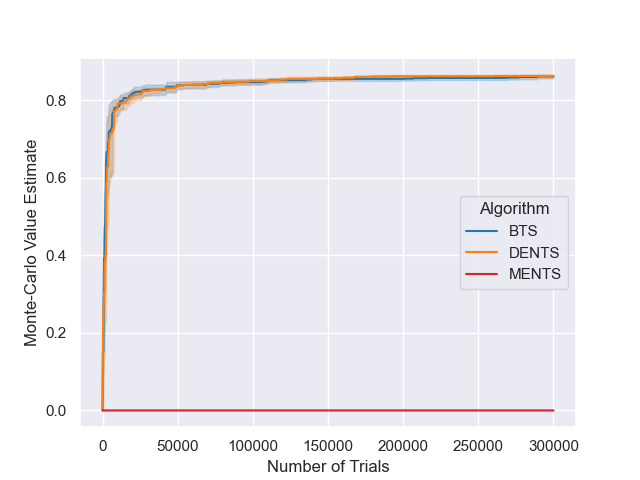
\includegraphics[width=\textwidth]{figures/temp/fl_sens/053_fl8_1_0_01.png}
                    \caption{$\alpha=1$}
                \end{subfigure}
                \begin{subfigure}[b]{0.32\textwidth}
                    \centering
                    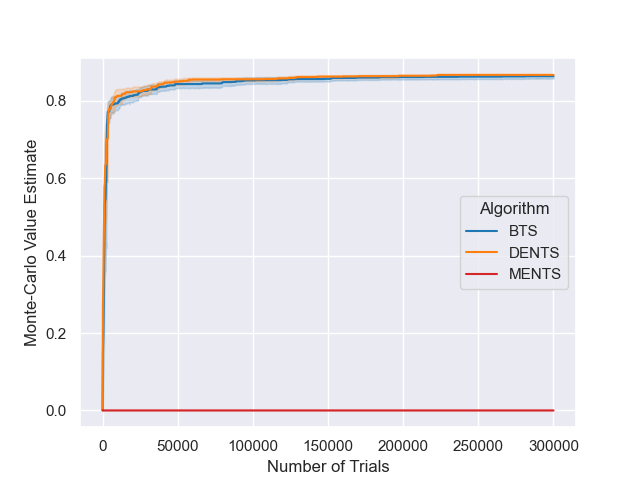
\includegraphics[width=\textwidth]{figures/temp/fl_sens/054_fl8_0_5_01.png}
                    \caption{$\alpha=0.5$}
                \end{subfigure}
                \begin{subfigure}[b]{0.32\textwidth}
                    \centering
                    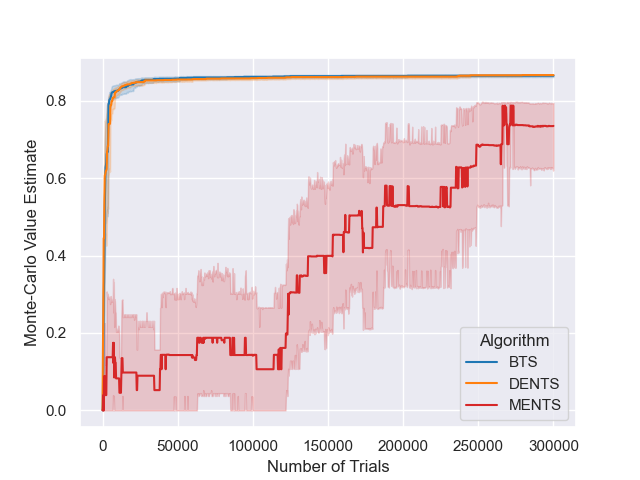
\includegraphics[width=\textwidth]{figures/temp/fl_sens/055_fl8_0_1_01.png}
                    \caption{$\alpha=0.1$}
                \end{subfigure}
                
                \begin{subfigure}[b]{0.32\textwidth}
                    \centering
                    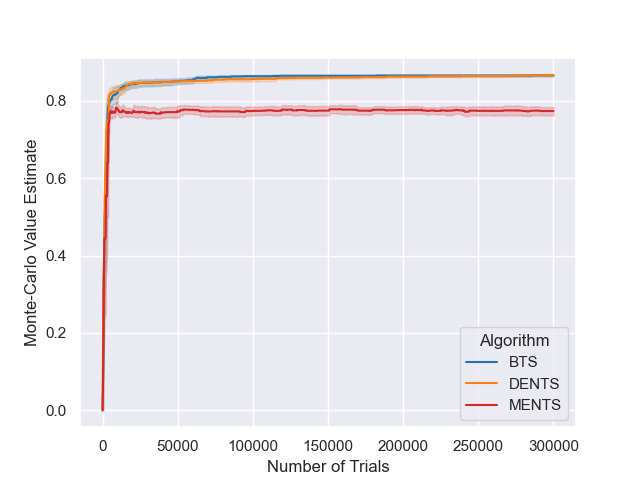
\includegraphics[width=\textwidth]{figures/temp/fl_sens/056_fl8_0_05_01.png}
                    \caption{$\alpha=0.05$}
                \end{subfigure}
                \begin{subfigure}[b]{0.32\textwidth}
                    \centering
                    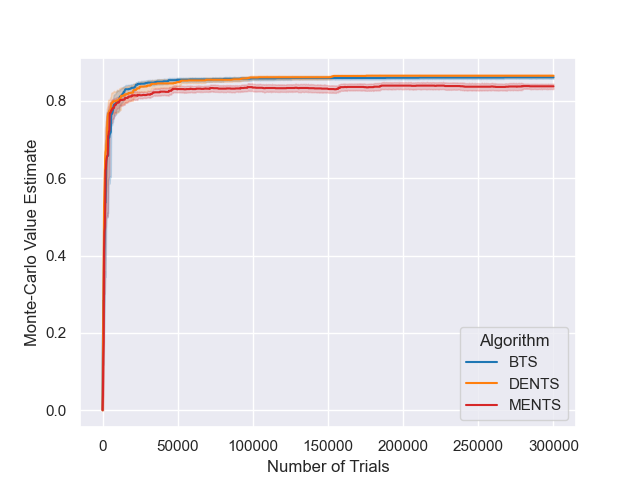
\includegraphics[width=\textwidth]{figures/temp/fl_sens/057_fl8_0_01_01.png}
                    \caption{$\alpha=0.01$}
                \end{subfigure}
                \begin{subfigure}[b]{0.32\textwidth}
                    \centering
                    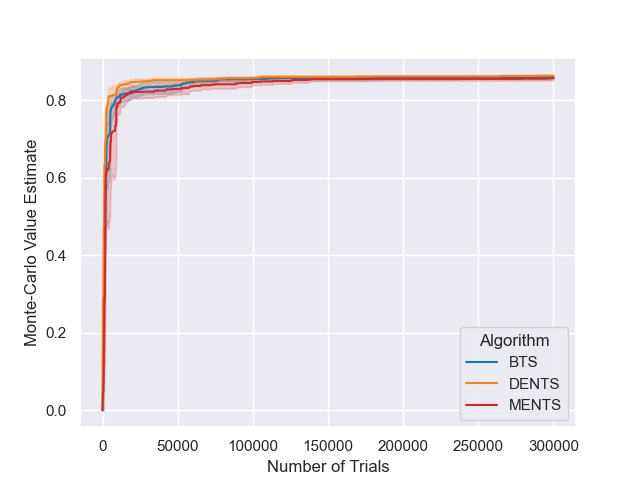
\includegraphics[width=\textwidth]{figures/temp/fl_sens/058_fl8_0_005_01.png}
                    \caption{$\alpha=0.005$}
                \end{subfigure}
                
                \caption{MENTS with a variety of temperatures on an 8x8 Frozen Lake environment. BTS and DENTS are included for reference. \todo{Update fig?}}
                \label{fig:fl_param_sens_ments}
            \end{figure}
            
            \begin{figure}
                \centering
                
                \begin{subfigure}[b]{0.32\textwidth}
                    \centering
                    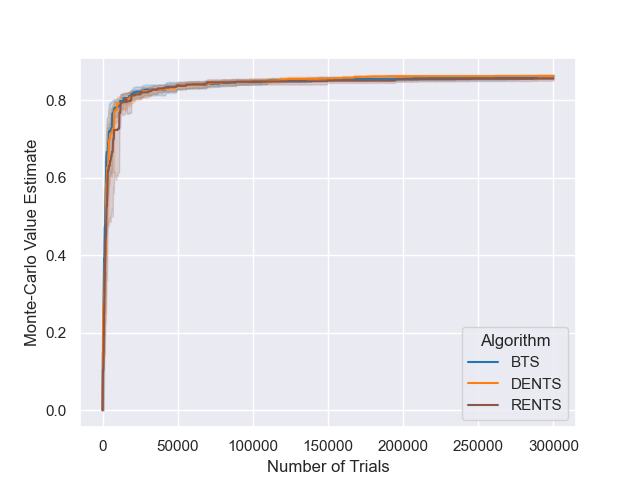
\includegraphics[width=\textwidth]{figures/temp/fl_sens/053_fl8_1_0_02.png}
                    \caption{$\alpha=1$}
                \end{subfigure}
                \begin{subfigure}[b]{0.32\textwidth}
                    \centering
                    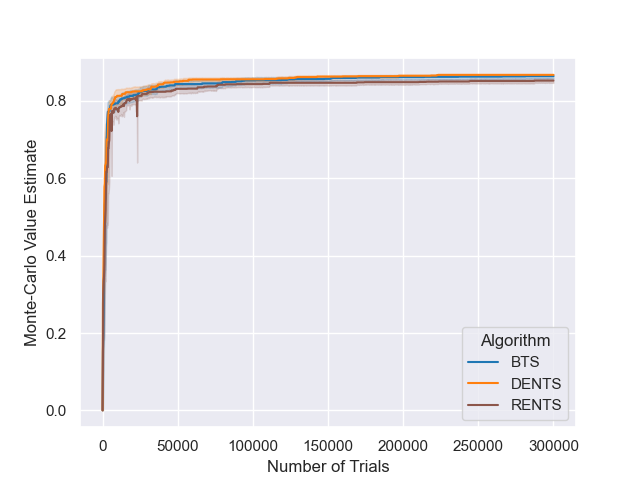
\includegraphics[width=\textwidth]{figures/temp/fl_sens/054_fl8_0_5_02.png}
                    \caption{$\alpha=0.5$}
                \end{subfigure}
                \begin{subfigure}[b]{0.32\textwidth}
                    \centering
                    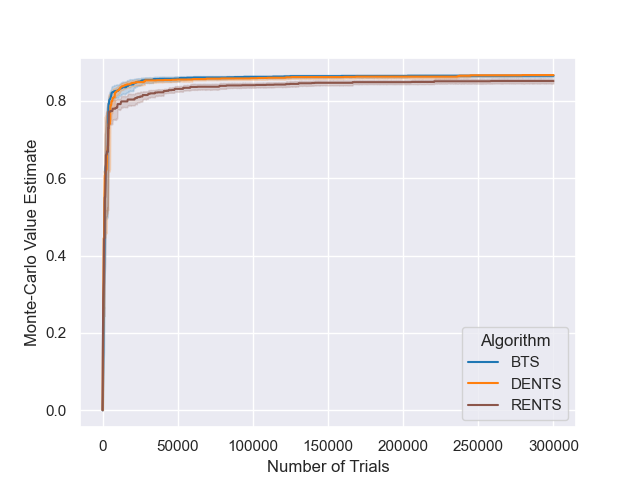
\includegraphics[width=\textwidth]{figures/temp/fl_sens/055_fl8_0_1_02.png}
                    \caption{$\alpha=0.1$}
                \end{subfigure}
                
                \begin{subfigure}[b]{0.32\textwidth}
                    \centering
                    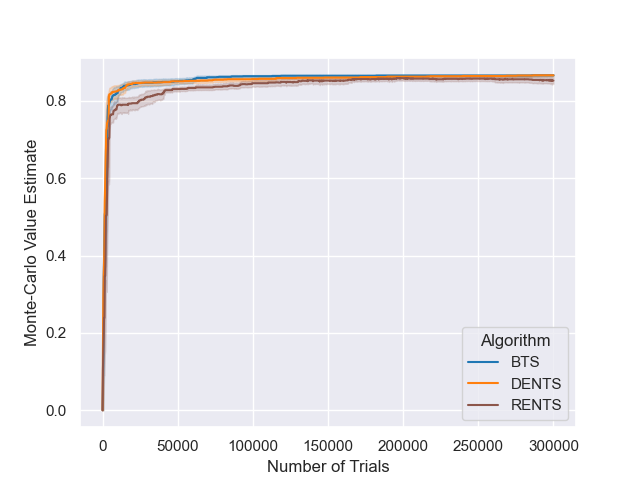
\includegraphics[width=\textwidth]{figures/temp/fl_sens/056_fl8_0_05_02.png}
                    \caption{$\alpha=0.05$}
                \end{subfigure}
                \begin{subfigure}[b]{0.32\textwidth}
                    \centering
                    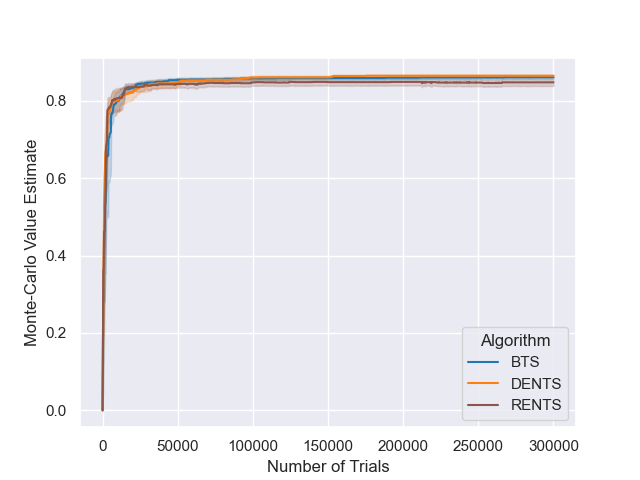
\includegraphics[width=\textwidth]{figures/temp/fl_sens/057_fl8_0_01_02.png}
                    \caption{$\alpha=0.01$}
                \end{subfigure}
                \begin{subfigure}[b]{0.32\textwidth}
                    \centering
                    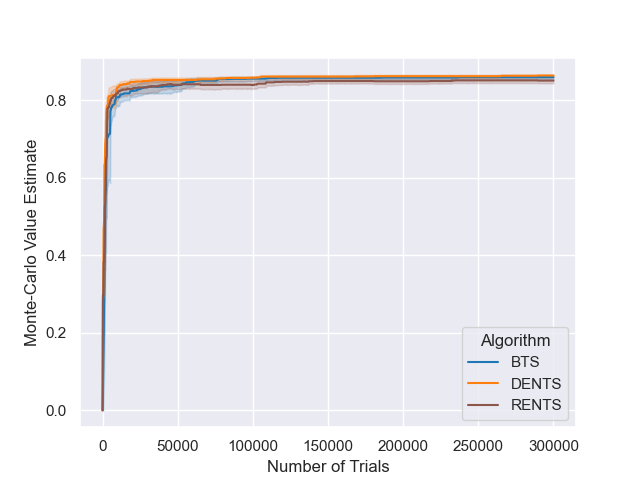
\includegraphics[width=\textwidth]{figures/temp/fl_sens/058_fl8_0_005_02.png}
                    \caption{$\alpha=0.005$}
                \end{subfigure}
                
                \caption{RENTS with a variety of temperatures on an 8x8 Frozen Lake environment. BTS and DENTS are included for reference. \todo{Update fig?}}
                \label{fig:fl_param_sens_rents}
            \end{figure}
            
            \begin{figure}
                \centering
                
                \begin{subfigure}[b]{0.32\textwidth}
                    \centering
                    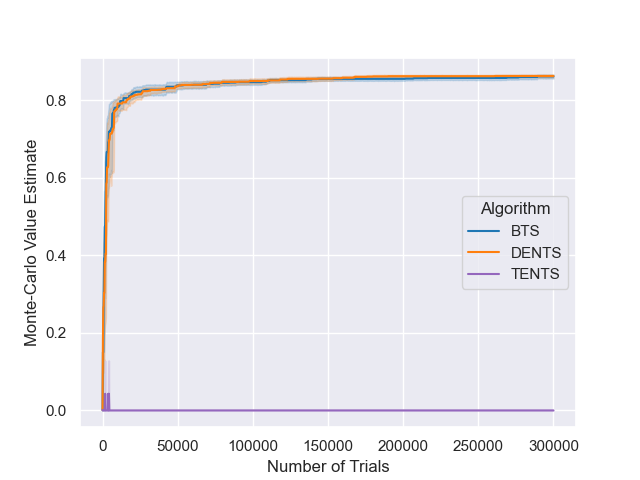
\includegraphics[width=\textwidth]{figures/temp/fl_sens/053_fl8_1_0_03.png}
                    \caption{$\alpha=1$}
                \end{subfigure}
                \begin{subfigure}[b]{0.32\textwidth}
                    \centering
                    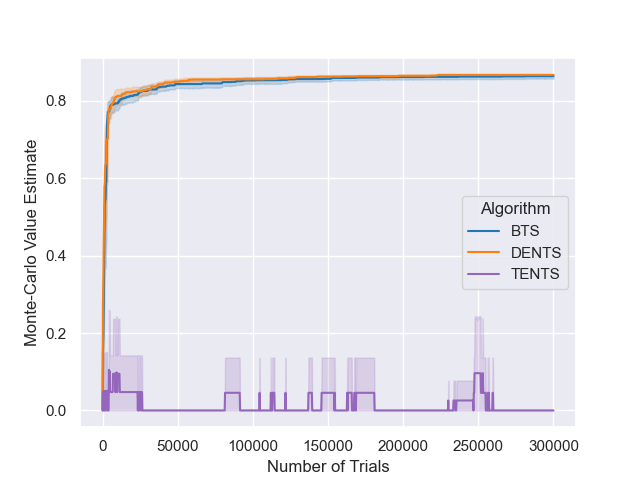
\includegraphics[width=\textwidth]{figures/temp/fl_sens/054_fl8_0_5_03.png}
                    \caption{$\alpha=0.5$}
                \end{subfigure}
                \begin{subfigure}[b]{0.32\textwidth}
                    \centering
                    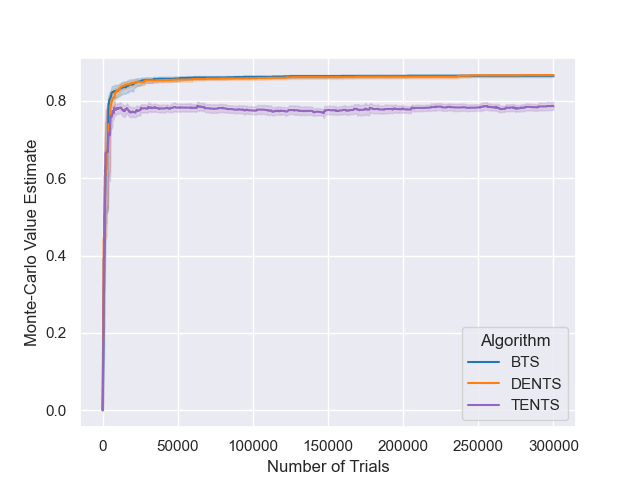
\includegraphics[width=\textwidth]{figures/temp/fl_sens/055_fl8_0_1_03.png}
                    \caption{$\alpha=0.1$}
                \end{subfigure}
                
                \begin{subfigure}[b]{0.32\textwidth}
                    \centering
                    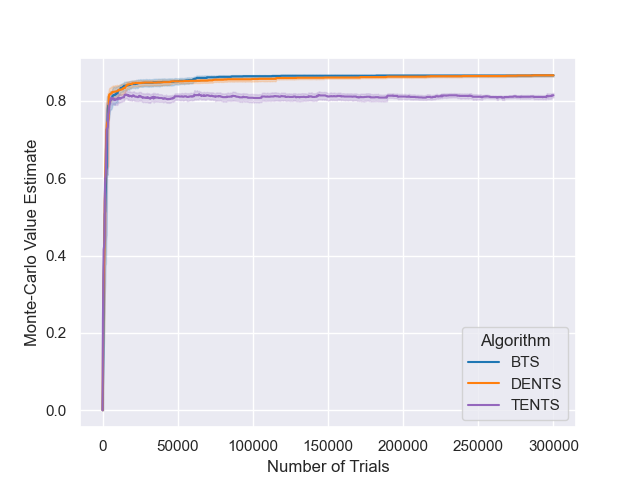
\includegraphics[width=\textwidth]{figures/temp/fl_sens/056_fl8_0_05_03.png}
                    \caption{$\alpha=0.05$}
                \end{subfigure}
                \begin{subfigure}[b]{0.32\textwidth}
                    \centering
                    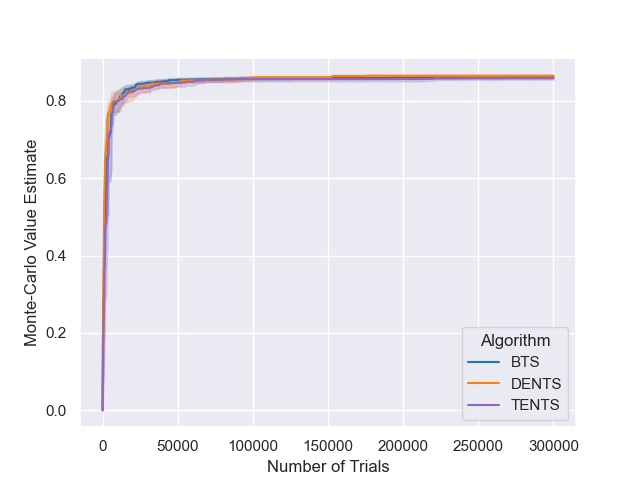
\includegraphics[width=\textwidth]{figures/temp/fl_sens/057_fl8_0_01_03.png}
                    \caption{$\alpha=0.01$}
                \end{subfigure}
                \begin{subfigure}[b]{0.32\textwidth}
                    \centering
                    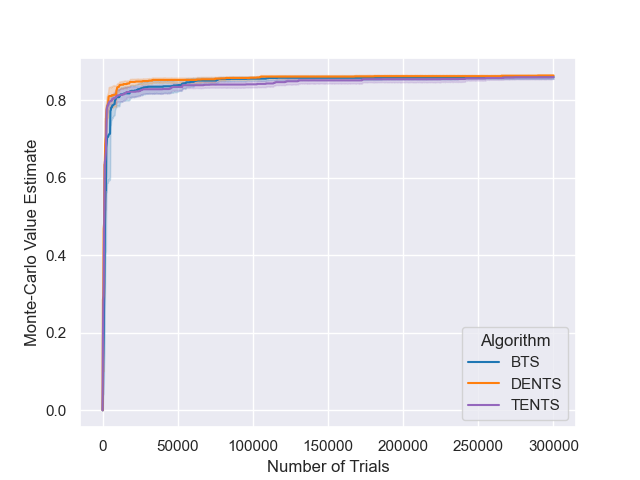
\includegraphics[width=\textwidth]{figures/temp/fl_sens/058_fl8_0_005_03.png}
                    \caption{$\alpha=0.005$}
                \end{subfigure}
                
                \caption{TENTS with a variety of temperatures on an 8x8 Frozen Lake environment. BTS and DENTS are included for reference. \todo{Update fig?}}
                \label{fig:fl_param_sens_tents}
            \end{figure}




        \subsubsection{DENTS with a constant $\beta$} \label{app:dents_mimic_ments}

            \htodo{this subsubsection currently just a c and p from neurips}

            \todo{Place this better? Or maybe just remove from thesis?}

            To empirically demonstrate that DENTS search policy can mimic the search policy of MENTS, we ran DENTS with $\alpha=1.0,\beta(m)=\alpha$ on the 10-chain environment, and compared it to MENTS with $\alpha=1.0$. We also ran DENTS with $\alpha=0.001, \beta(m)=\alpha$ in the Frozen Lake environment, and compared it to MENTS with $\alpha=0.001$ which is what was selected in the hpyerparameter search (Appendix \ref{app:hps}). Results are given in Figure \ref{fig:dbments}. Note that in the 10-chain, only MENTS has a dip in performance initially, which is due to the two algorithms using different recommendation policies.
            
            
            \begin{figure*}
                \centering
                \begin{subfigure}[b]{0.49\textwidth}
                    \centering
                    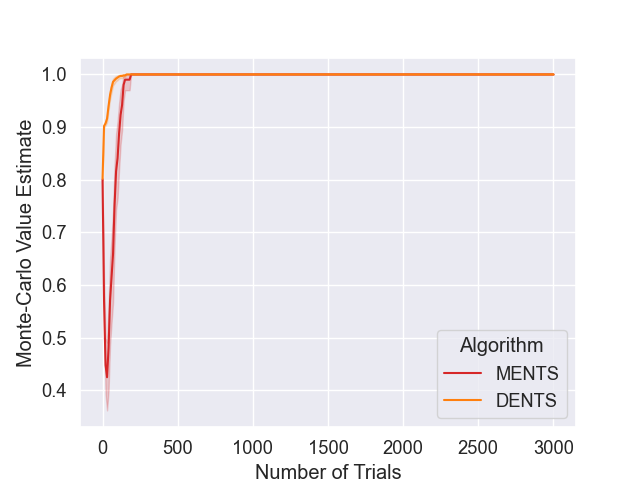
\includegraphics[width=\textwidth]{figures/temp/dbments/dbments_dchain.png}
                    \caption{10-chain.}
                \end{subfigure}
                \begin{subfigure}[b]{0.49\textwidth}
                    \centering
                    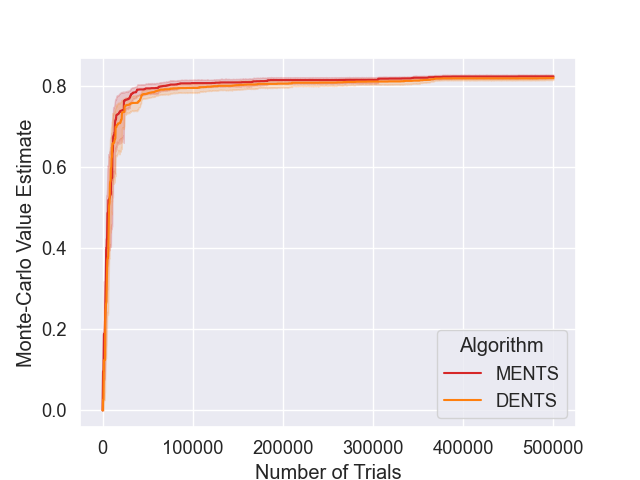
\includegraphics[width=\textwidth]{figures/temp/dbments/dbments_fl.png}
                    \caption{Frozen Lake.}
                \end{subfigure}
                \caption{Comparing DENTS with MENTS, by setting $\beta_{\text{DENTS}}(m)=\alpha_{\text{MENTS}}, \alpha_{\text{DENTS}}=\alpha_{\text{MENTS}}$, where $\alpha_{\text{MENTS}}$ is the temperature used for MENTS, and $\alpha_{\text{DENTS}},\beta_{\text{DENTS}}$ are the temperatures used by DENTS.  \todo{Update fig?}}
                \label{fig:dbments}
            \end{figure*}



        \subsubsection{Gridworld Results}

            \htodo{this subsubsection currently just a c and p from neurips}

            \todo{Ref the above} We used an 8x12 Frozen Lake environment and a 6x6 Sailing Problem for evaluation

            Each algorithm is run 25 times on each environment and evaluated every 250 trials using 250 trajectories. 
            A horizon of 100 was used for Frozen Lake and 50 for the Sailing Problem.

            In Frozen Lake (Figure \ref{fig:fl}), entropy proved to be a useful exploration bonus for the \textit{sparse reward}. Values in UCT and BTS remain at zero until a trial successfully reaches the goal. However, entropy guides agents to avoid trap states, where the entropy is zero. DENTS was able to perform similarly to MENTS, and BTS was able to improve its policy over time more than UCT.

            In the Sailing Problem (Figure \ref{fig:sp}) UCT performs well due to the dense reward. BTS and DENTS also manage to keep up with UCT. MENTS and TENTS appear to be slightly hindered by entropy in this environment. The relative entropy encourages RENTS to pick the same actions over time, so it tends to pick a direction and stick with it regardless of cost.
            
            Finally, BTS and DENTS were able to perform well in both domains with a sparse and dense reward structure, whereas the existing methods performed better on one than the other, hence making BTS and DENTS good candidates for a general purpose MCTS algorithm.
            
            \begin{figure*}
                \centering
                \begin{subfigure}[b]{0.49\textwidth}
                    \centering
                    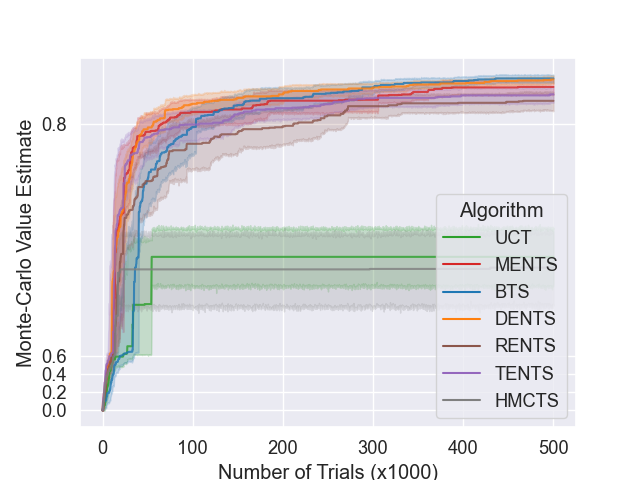
\includegraphics[width=\textwidth]{figures/temp/grid/fl.png}
                    \caption{8x12 Frozen Lake.}
                    \label{fig:fl}
                \end{subfigure}
                \begin{subfigure}[b]{0.49\textwidth}
                    \centering
                    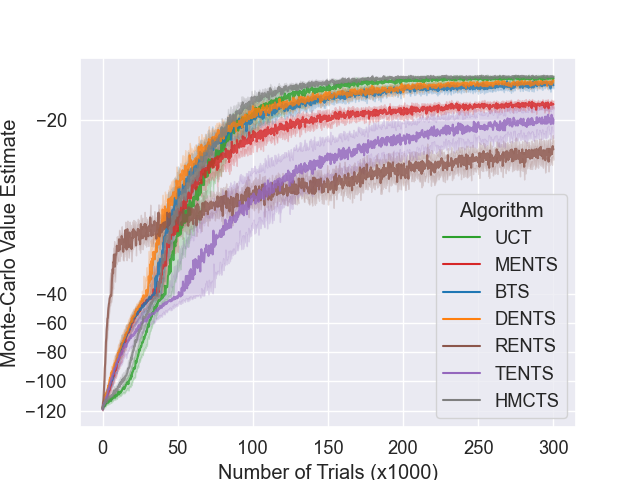
\includegraphics[width=\textwidth]{figures/temp/grid/s.png}
                    \caption{6x6 Sailing Problem.}
                    \label{fig:sp}
                \end{subfigure}
                \caption{Results for gridworld environments. Further results are given in Appendix \ref{app:hps}. \todo{update fig?}}
                \label{fig:gridworld_results}
            \end{figure*}





        \subsubsection{Go Results}

            \htodo{this subsubsection currently just a c and p from neurips}
        
            In each match, each algorithm played $50$ games as black and $50$ as white. \todo{this was moved from another parahraph} 

            Results of the round-robin are summarised in Table \ref{table:go_results}, and we discuss how parameters were selected in Appendix \ref{app:go_hps}. BTS was able to run the most trials per move and beat all of the other algorithms other than DENTS which it drew. We used the optimisations outlined in Appendix \ref{app:alias} which allowed the Boltzmann search algorithms to run significantly more trials per move than PUCT. 
            BTS and DENTS were able to beat PUCT with results of 57-43 and 58-42 respectively. Using entropy did not seem to have much benefit in these experiments, as can be witnessed by MENTS only beating TENTS, and DENTS drawing 50-50 with BTS. This is likely because the additional exploration provided by entropy is vastly outweighed by utilising the information contained in the neural networks $\tilde{V}$ and $\tilde{\pi}$. %DENTS was able to take more games from PUCT as white, so Shannon entropy may be useful in obtaining an advantage as white.
            Interestingly RENTS had the best performance out of the prior works, losing 43-57 to PUCT, and the use of relative entropy appears to take advantage of a heuristic for Go that the RAVE \todo{cite}%\cite{rave}
             algorithm used: the value of a move is typically unaffected by other moves on the board.
            
            To validate the strength of our PUCT agent, we also compared it directly with KataGo \todo{cite}%\cite{katago}
            , limiting each algorithm to 1600~trials per move. Our PUCT agent won 61-39 in 9x9 Go, and lost 35-65 in 19x19 Go, suggesting that our PUCT agent is strong enough to provide a meaningful comparison for our other general purpose algorithms. Finally, note that we did not fine-tune the neural networks, so the Boltzmann search algorithms directly used the networks that were trained for use in PUCT.
            % The algorithms using $O(|\cl{A}|)$ entropy backups were still able to run a competitive number of trials per move, because in the multi-threaded search the additional exploration led to less contention over values, and hence threads could spend less time waiting.
            %Overall, three algorithms were able to beat PUCT: RENTS won 60-40 and appears to take advantage of the value of a move typically being unaffected by other moves on the board, which the RAVE algorithm took advantage of \cite{rave}; BTS and DENTS had convincing wins of 81-19 and 89-11 over PUCT respectively and demonstrate the effectiveness of prioritising exploration more in planning. As DENTS was able to take more games from PUCT as white, Shannon entropy seems to be useful in obtaining an advantage as white. Unfortunately, DENTS wasn't able to outperform BTS with a match score of 47-53, which could be due to $\beta$ being difficult to tune, or potentially Shannon entropy is not helpful for Go. If we combined DENTS with relative entropy, the resulting algorithm likely would have beaten BTS.
            
          	

        \begin{table*}[]
        \centering   
		    \begin{tabular}{l|cccccc|c} 
		        \textbf{Black \textbackslash White}     & PUCT  & AR-M  & AR-R  & AR-T  & AR-B  & AR-D   & Trials/move\\ 
		        \hline
		                                PUCT            &   -   & 33-17 & 27-23 & 42-8  & 17-33 & 15-35  & 1054 \\
		                                AR-MENTS        & 12-48 &   -   & 13-37 & 38-12 & 10-40 & 12-38  & 4851\\
		                                AR-RENTS        & 20-30 & 24-26 &   -   & 39-11 & 18-32 & 14-36  & 3672 \\
		                                AR-TENTS        &  8-42 & 11-39 &  9-41 &   -   &  6-44 & 10-40  & 5206 \\
		                                AR-BTS          & 25-25 & 35-15 & 31-19 & 34-16 &   -   & 15-35  & 5375 \\
		                                AR-DENTS        & 23-27 & 36-14 & 29-21 & 36-14 & 15-35 &   -    & 4677 \\         
		    \end{tabular}
            \caption{Results for the Go round-robin tournament. The first column gives the agent playing as black. The final column gives the average trials run per move across the entire round-robin. In the top row, we abbreviate the algorithm names for space.\label{table:go_results}}
        \end{table*}



































        
            
            
            
            
            






























\section{Theoretical Results}
\label{sec:4-5-theory}




    \todo{First thing to do in this section is write up the results for what we're showing (in the chapter). Then write up the results we're showing in the appendix. Then move the proofs needed to build the results showing in this chapter. Then dump all of the remainder in the appendix.}



    \todo{Double check appendix B coverered properly here}






    \begin{table*}[]
        \centering
        \begin{tabular}{l|c|c|c}
                    
                & DENTS   
                & AR-DENTS    
                & MENTS   \\
            \hline
            \todo{}$\psi$ %Val estimate rec policy 
                &    
                & $\alphaardents(m)\rightarrow 0$, $\frac{\betaardents(m)}{\alphaardents(m)}\rightarrow 0$
                & $\alphaments<\frac{\Delta_{\cl{M}}}{3H\log |\cl{A}|}$ \todo{H consistent with thtspp} \\
            \hline
            \todo{}$\texttt{mv}$ %Most visit rec policy 
                & $\frac{\betadents(m)}{\alphadents(m)}\rightarrow 0$
                & $\alphaardents(m)\rightarrow 0$, $\frac{\betaardents(m)}{\alphaardents(m)}\rightarrow 0$
                & $\alphaments<\frac{\Delta_{\cl{M}}}{3H\log |\cl{A}|}$ \todo{H consistent with thtspp} \\
        \end{tabular}
        \caption{\todo{Summary of conditions for algorithms to be consistent.} 
            \label{tab:4:summary_consistency_conditions}}
    \end{table*}
    







    \todo{Here we should front load the ``main results'' of the theory section, and write them up in a story, for example showing that DENTS can always be made to converge, although you may have to tune results for good performance in practise. THEN give an outline of how the proofs are laid out, and if the proofs are in the appendix or the rest of this chapter.}



    \todo{Below until end of list is some notes pre writing up theory and bit copied from the neurips paper directly}

    Should we try to add a result about most visited? Where will be concentration bounds around the number of visits being proportional to the values. So think can bootstrap those proofs.

    - Generalise the AR proof to say that for decaying search functions still work (as long as they are bounded)
    - Have a result that using most visited is theoretically sound

    The Neurips paper proof section was structured as follows:
    \begin{enumerate}
        \item First, in Section \ref{app:mcts_process} we revisit MCTS as a stochastic process, defining some additional notation that was not useful in the main body of the paper, but will be for the following proofs;
        \item Second, in Section \ref{app:preliminaries} we introduce preliminary results, that will be useful building blocks for proofs in later Theorems;
        \item Third, in Section \ref{app:soft_learning_results} we show some general results about soft values that will also be useful later;
        \item Fourth, in Section \ref{app:simple_regret_results} simple regret is then revisited, and we show that any bounds on the simple regret of a policy are equivalent to showing bounds on the simple regret of an action;
        \item Fifth, in Section \ref{app:q_result} we show in a general way, that if a value function admits a concentration inequality, then the corresponding Q-value function admits a similar concentration inequality;
        \item Sixth, in Section \ref{app:ments_results} we show concentration inequalities for MENTS about the optimal soft values, and give bounds on the simple regret of MENTS, provided the temperature parameter is sufficiently small;
        \item Seventh, in Sections \ref{appsec:dents_proofs} and \ref{appsec:bts_proofs} we also provide concentration inequalities around the optimal standard values for BTS and DENTS, and give simple regret bounds, irrespective of the temperature paramters;
        \item Finally, in Section \ref{sec:ar_proofs} we consider results that are relavant for the algorithms using average returns from Section \ref{app:average_returns}.
    \end{enumerate}













%%%%
% THEORY - Stochastic Processes Definitions
%%%%



\todo{Some comment about using a policy of the form XXX will be refered to a Boltzmann MCTS Process.}



\subsection{MCTS As A Stochastic Process}
    Now the MENTS, BTS and DENTS are written as a stochastic process, where values are indexed (with a superscript) by the number of times that the corresponding node has been visited. For completeness and reference, the stochastic processes for \todo{UCT?}, MENTS, BTS and DENTS are given below.
    


    \todo{change m to n, and use mth when need to reason about prev trials (whole subsection)}

    When reasoning about a \textit{MCTS stochastic process} the following notations will be helpful.
    \begin{itemize}
        \item 
            The search policy used on the $m$th trial is $\pi^m$, and if the process were stopped after $m$ trials, the recommendation policy that the algorithm would output is denoted $\psi^m$. Where if the process is run for $n$ trials, then $m$ ranges from $1$ to $n$.
        \item 
            The $m$ trajectory sampled is $\tau^m=(s_0^m,a_0^m,...,s_{h-1}^m,a_{h-1}^m,s_{h}^m)$ \todo{add reward, also make it h subscript m instead of h?}, and is sampled using the search policy $\tau^m \sim \pi^m$ (that is $a^m_i \sim \pi^m(\cdot|s^m_i)$ and $s^m_{i+1} \sim p(\cdot | s^m_i, a^m_i)$). \todo{comment that $k$th trial is run until h where s subscript h is termal in some thtspp sense. Comment about how the superscripts on s a and r will be used when necessary, but not always}
        \item 
            The search tree after $m$ trials is denoted $\cl{T}^m$, the initial search tree is $\cl{T}^0=\{s_0\}$, and $\cl{T}^k = \cl{T}^{k-1} \cup \tau^k$.
    \end{itemize}

    When making arguments that apply to multiple algorithms the general policies $\pi$ and $\psi$ will be used, and when making arguments about specific algorithms the subscripts will be used, such as $\pibts$. Note that superscript is used to index with respect to the trial, and superscript with parenthasis is used to denote the number of visits.

    In the proofs of following sections, it will be useful to write the number of times state~$s$ was visited in the first $m$ trials as $N(s,m)$, and the number of times action~$a$ was selected from state~$s$ in the first m trials as $N(s,a,m).$ Additionally, it will be useful to write these quantities in terms of indicator random variables. 
    
    Let $T(s_t,m)$ (and $T(s_t,a_t,m)$) be the set of trajectory indices that $s_t$ was visited on (and action $a_t$ selected) in the first $m$ trials, that is: \todo{this can avoid using s subscript t}
    %
    \begin{align}
        T(s_t,m) &= \{i | i\leq m, s^i_t = s_t \} \\
        T(s_t,a_t,m) &= \{i | i\leq m, s^i_t = s_t, a^i_t = a_t \}.
    \end{align}
    %
    This allows the counts $N^m(s_t),$ $N^m(s_t,a_t)$ and $N^m(s_{t+1})$ (with $s_{t+1}\in\suc{s_t}{a_t}$) to be written as sums of indicator random variables in the following ways:
    %
    \begin{align}
        N(s_t,m) &= \sum_{i=1}^m \one[s^i_t=s_t] = |T(s_t,m)|, \\
        N(s_t,a_t,m) &= \sum_{i=1}^m \one[s^i_t=s_t,a^i_t=a_t] = |T(s_t,a_t,m)|, \\ 
        N(s_t,a_t,m) &= \sum_{i\in T(s_t,m)} \one[a^i_t = a_t], \label{appeq:nsa_sum} \\
        N(s_{t+1},m) &= \sum_{i\in T(s_t,a_t,m)} \one[s^i_{t+1} = s_{t+1}]. \label{appeq:ns_sum}
    \end{align}
    %
    Additionally, the assumption that for any two states $s,s'\in\cl{S}$ \todo{double check use calligraphic S for state space?} that $s=s'$ if and only if the trajectories leading to them are identical is made. This assumption is purely to simplify notation, so that nodes in the tree have a one-to-one correspondence with states (or state-action pairs). \todo{move this up}
        
        
        
        

    \todo{do we do anything at all with the UCT process?}
    % \subsubsection{The UCT process.} 
    % 	The UCT search policy can be defined as:
    % %
    % \begin{align}
    %      \pi_{\textnormal{UCT}}^n(s_t) &= \max_{a\in\cl{A}} \text{UCB}^n(s_t,a), \\
    %      \text{UCB}^n(s_t, a) &= 
    %     		\begin{cases}
    %     			\infty & \text{if } N(s_t,a)=0 \\
    %     			\bar{Q}^{N(s_t,a)}(s_t, a)+c \sqrt{\frac{\log N(s_t)}{N(s_t, a)}} & \text{if } N(s_t,a)>0
    %     		\end{cases}
    % \end{align}
    % %
    % \noindent where, after $n$ trials, $\bar{Q}^{N(s,a)}(s,a)$ is the empirical estimate of the value at node $(s,a)$, where action~$a$ has been selected $N(s, a)$ from state~$s$. The backup consists of updating empirical estimates for $t=h-1,...,0$:
    % %
    % \begin{align}
    %     \bar{V}^{N(s_t)+1}(s_t) &= \bar{V}^{N(s_t)}(s_t) + \frac{\bar{R}(t) - \bar{V}^{N(s_t)}(s_t)}{N(s_t) + 1}, \label{appeq:uct_vbar} \\
    %     \bar{Q}^{N(s_t,a_t)+1}(s_t, a_t) &= \bar{Q}^{N(s_t,a_t)}(s_t, a_t) + \frac{\bar{R}(t) - \bar{Q}^{N(s_t,a_t)}(s_t, a_t)}{N(s_t, a_t) + 1}, \label{appeq:uct_qbar}
    % \end{align}
    % %
    % \noindent where $\bar{R}(t) = V^{\text{init}}(s_h) + \sum_{i=t}^{h-1} R(s_i,a_i)$, and values are initialised as $\bar{V}^1(s)=V^{\text{init}}(s)$ and $\bar{Q}^0(s,a)=0$. 
    

    
    
    
    \subsubsection{The MENTS Process}
    
    Below is a complete summary of the MENTS process, for reference. On the $m$th trial, the MENTS process follows the search policy:

    \todo{make ments section in ch2 use consistent definitions of alphaments, lambdaments and so on}

    \begin{align}
        \mpiments{m}(a|s) &= (1-\mlambdaments{m})\mrhoments{m}(a|s) + \frac{\mlambdaments{m}}{|\cl{A}|}, 
                    \label{appeq:ments_soft_policy} \\ 
        \mrhoments{m}(a|s) &= \exp\left(
            \frac{1}{\alphaments}\left(\mQments{N(s,a,m-1)}(s,a)-\mVments{N(s,m-1)}(s)\right)\right). \\
        \lambda^m(s,x) &= \min\left(1, \frac{x}{\log(e+N(s,m-1))}\right),
    \end{align}
    %
    where $\epsments\in(0,\infty)$ is an exploration parameters, and $\alphaments$ is the temperature parameter. 

    The $m$th trajectory is sampled using the search policy: $\tau^m \sim \piments^m$. Letting $\tau^m=(s_0,a_0,r_0,...,s_{h-1},a_{h-1},r_{h-1},s_{h})$, the MENTS value estimates are computed using backups for $t=h-1, ..., 0$: \todo{either add the superscript m into every s and a, or update words to say implicit}
    \begin{align}
        \mVments{N(s_t,m)}(s_t) &= 
            \alphaments \log \sum_{a\in\cl{A}} \exp \left(
                \frac{1}{\alphaments}\mQments{N(s_t,a,m)}(s_t,a) \right), \label{appeq:soft_v_backup} \\
        \mQments{N(s_t,a_t,m)}(s_t,a_t) &= 
            R(s_t,a_t) + \sum_{s'\in\suc{s}{a}} \left( 
                \frac{N(s',m)}{N(s_t,a_t,m)} \mVments{N(s',m)}(s') \right). \label{appeq:soft_q_backup}
    \end{align}

    \todo{also want something about initialisation and everything in line with thtspp}
    %
    % The soft (Q-)values are initialised as $\Vst{s}{1}=V^{\text{init}}(s)$ and $\Qst{s}{a}{0}=Q^{\text{init}}_{\sft}(s)$ (typically $Q^{\text{init}}_{\sft}(s)=0$).

    \todo{recommendation policies and some comment about it being the soft values used?}
    \begin{align}
        \mpsiments{m}(s) &= \argmax_{a\in\cl{A}}\mQments{N(s,a,m)}(s,a), \\
        \mmvments{m}(s) &= \argmax_{a\in\cl{A}} N(s,a,m).
    \end{align}










\subsubsection{The DENTS Process}

    \todo{this whole sections math is pretty mess and a struggle to fit onto one line at a time. Maybe it suffices to just wordily describe the values of the sufixed values?}

    Follow policy: 
    %
    \todo{add more wordy things. Some things we said here before were: (1) defining beta} $\beta : \bb{R}\rightarrow [0,\infty)$ be a bounded function; \todo{(2) defined epsilon as exploration policy; (3) in Neurips we defined the propto version of rho and also the full version saying ``becasue we need to reason about the search policy we give the exact form,'' for the moment I've kept both. I think just copy the full version where relevent in the proofs.}
    %
    \begin{align}
        \mpidents{m}(a|s) &= (1-\mlambdadents{m})\mrhodents{m}(a|s) + \frac{\mlambdadents{m}}{|\cl{A}|}, 
            \label{appeq:dents_search_policy}  \\
        \mrhodents{m}(a|s) &\propto \exp\left(\frac{1}{\alphadents(N(s,m))}
            \left(\mQdents{N(s,a,m-1)}(s,a) + \betadents(N(s,m))\mHQdents{N(s,a,m-1)}(s,a) \right)\right). \\
        \mrhodents{m}(a|s) &= \frac{
            \exp\left(\frac{1}{\alphadents(N(s,m))}\left(
                \mQdents{N(s,a,m-1)}(s,a) + \betadents(N(s,m))\mHQdents{N(s,a,m-1)}(s,a)   \right)\right)
            }{\sum\limits_{a'\in\cl{A}} \exp\left(\frac{1}{\alphadents(N(s,m))}\left(
                \mQdents{N(s,a',m-1)}(s,a') + \betadents(N(s,m))\mHQdents{N(s,a',m-1)}(s,a')  \right)\right)}.  
            \label{appeq:full_rho} \\
        \lambda^m(s,x) &= \min\left(1, \frac{x}{\log(e+N(s,m-1))}\right), 
    \end{align}

    The $m$th trajectory is sampled using the search policy: $\tau^m \sim \piments^m$. Letting $\tau^m=(s_0,a_0,r_0,...,s_{h-1},a_{h-1},r_{h-1},s_{h})$, the DENTS value and entropy estimates are computed using backups for $t=h-1, ..., 0$: \todo{either add the superscript m into every s and a, or update words to say implicit}
    \begin{align}
        \mQdents{N(s_t,a_t,m)}(s_t,a_t) &= 
            R(s_t,a_t) + \sum_{s' \in \suc{s_t}{a_t}} \left( 
                \frac{N(s',m)}{N(s_t,a_t,m)} \mVdents{N(s',m)}(s') \right), 
            \label{appeq:dp_q_backup} \\ 
        \mVdents{N(s_t,m)}(s_t) &=\max_{a\in\cl{A}} \mQdents{N(s_t,a,m)}(s_t,a), 
            \label{appeq:dp_v_backup} \\
        \mHQdents{N(s_t,a_t,m)}(s_t,a_t) &= 
            \sum_{s'\in \suc{s_t}{a_t}} \frac{N(s',m)}{N(s_t,a_t,m)} \mHVdents{N(s',m)}(s'), \\
        \mHVdents{N(s_t)}(s_t) &= 
            \cl{H}(\mpidents{m}(\cdot | s_t)) 
                + \sum_{a\in\cl{A}} \mpidents{m}(a_t|s_t)\mHQdents{N(s_t,a_t,m)}(s_t,a_t).
    \end{align}

    \todo{also want something about initialisation and everything in line with thtspp}
    %
    % The (Q-)values are initialised as $\Vt{s}{1}=V^{\text{init}}(s)$ and $\Qt{s}{a}{0}=Q^{\text{init}}_{\sft}(s)$ (typically $Q^{\text{init}}_{\sft}(s)=0$). The entropy values are initialised as $\cl{H}_Q^{0}(s,a)=0$ and $\cl{H}_V^{1}(s) = \cl{H}(\pi^n_{\text{DENTS}}(\cdot | s_t))$, where the node for $s$ is created on the $n$th trial

    \todo{recommendation policies word stuff}
    \begin{align}
        \mpsidents{m}(s) &= \argmax_{a\in\cl{A}}\mQdents{N(s,a,m)}(s,a), \\
        \mmvdents{m}(s) &= \argmax_{a\in\cl{A}} N(s,a,m).
    \end{align}

    \todo{From the neurips, also wrote the following (everything left in this subsubsection is copied and cleaned up, but probably needs a proof read)} Let $\mVrhodents{N(s)}(s)$ be defined as the value:
    %
    \begin{align}
        \mVrhodents{N(s)}(s) = &
            \alphadents(N(s,m)) \log \Bigg[ \sum_{a'\in\cl{A}} \exp\bigg(\frac{1}{\alphadents(N(s,m))}
                \big(\mQdents{N(s,a')}(s,a') \nonumber \\
            &+ \betadents(N(s,m))\mHQdents{N(s,a')}(s,a') \big)\bigg)\Bigg], \label{appeq:v_rho}
    \end{align} 
    %
    and notice that the value of $\exp(\mVrhodents{N(s,m)}(s)/\alphadents(N(s,m)))$ is equal to the denominator in Equation (\ref{appeq:full_rho}), and so by rearranging we can write $\mrhodents{m}$ as 
    %
    \begin{align}
        \mrhodents{m}(a|s) = 
            \exp\left(\frac{1}{\alphadents(N(s,m))}\left(
                \mQdents{N(s,a,m)}(s,a) 
                + \betadents(N(s,m))\mHQdents{N(s,a,m)}(s,a) 
                - \mVrhodents{N(s,m)}(s) \right)\right), \label{appeq:rho_concise}
    \end{align}
    % 
    and subsequently, the full DENTS policy can be written as:
    \begin{align}
        \mpidents{m}(a|s) = (1-\lambda(s,m))\exp\left(\frac{1}{\alphadents(N(s,m))}\left(\mQdents{N(s,a,m)}(s,a) + \betadents(N(s,m))\mHQdents{N(s,a)}(s,a) - \mVrhodents{N(s)}(s) \right)\right) + \frac{\lambda(s,m)}{|\cl{A}|}. \label{appeq:dents_search_policy_exact} 
    \end{align}








\subsubsection{The AR-DENTS Process}
        









\subsubsection{The (AR-)BTS process.}

    The (AR-)BTS process is a special case of the (AR-)DENTS process when $\betadents(x)=0$. As such, results about BTS will be corollaries from proofs about the (AR-)DENTS process.












%%%%
% THEORY - Defns
%%%%

\subsection{Preliminaries}

    \begin{defn}
        A sequence of random variables $X_i$ \textnormal{converges in probability} to a random variable $X$, written as $X_n \rap X$, if for all $\varepsilon>0$ the following holds:
        \begin{align}
            \Pr\left(\left|X_n - X\right| > \varepsilon\right) \rightarrow 0 \ \text{as} \ n \rightarrow \infty.
        \end{align}
    \end{defn}

    \begin{defn}
        A sequence of random variables $X_i$ \textnormal{converges almost surely} to a random variable $X$, written as $X_n \raas X$, if the following holds:
        \begin{align}
            \Pr\left(\lim_{n\rightarrow\infty} X_n = X\right) = 1.
        \end{align}
    \end{defn}


    \htodo{had this (commented out below) in the Neurips paper, but probably want to actually just define convergence in probability here, and say ``letting n tend to infinity'' gives the convergence in probability result.}


% Note that all of our concentration inequalities imply a convergence in probability. For example, we explicitly demonstrate this in Corollary \ref{cor:sftq_convg}.
        
% \begin{corollary} \label{cor:sftq_convg}
%         $\Qst{s_t}{a_t}{N(s_{t},a_t)}\rap \Qss{s_t}{a_t}$
% \end{corollary}
% \begin{proof}
%         This follows from the concentration inequalities shown in Lemma \ref{lem:stochastic_step} and Theorem \ref{thrm:ments_val_converge}. As the RHS of the bound tend to zero as $n\rightarrow\infty$, these concentration inequalities follow by taking the limit $n\rightarrow\infty$:
%         \begin{align}	
%         \lim_{n\rightarrow\infty} \Pr\left(\left| \Qst{s_{t}}{a_t}{N(s_{t},a_t)} - \Qss{s_t}{a_t} \right| > \varepsilon \right) 
%             &\leq \lim_{n\rightarrow\infty}  C\exp\left( -k\varepsilon^2 N(s_{t}) \right) \\
%             &= 0.
%         \end{align}
%     \end{proof}







%%%%
% THEORY - Preliminaries (for exp bound stuff)
%%%%

\subsection{Preliminaries - Exp}

    






    \todo{This section contains things related to exponential bounds, which might move to appendix}
    This subsection contains lemmas that will be useful in multiple times and are used to avoid repeating the same argument multiple times. 

    
    \todo{change m to n, and use mth when need to reason about prev trials (whole subsection)}





    Firstly it will be that the union of exponentially unlikely events is also exponentially unlikely, and that the intersection of exponentially likely events is exponentially likely. Although this is a special case of the union bound \todo{ref?} \todo{it is stated here so that it can be referenced, because this fact is used regularly }
    %
    \todo{Some comment about how this is just a special case of the union bound (and ref that?) and also }
    %
    \begin{lemma} \label{lem:union_bound}
        Let $A_1,...,A_{\ell}$ be some events that satisfy for $1\leq i \leq \ell$ the inequality $\Pr(\lnot A_i) \leq C_i\exp(-k_i)$ then:
        \begin{align}
            \Pr\left(\bigcup_{i=1}^\ell \lnot A_i\right) &\leq C\exp(-k), \label{appeq:comb_exp_like} \\
            \Pr\left(\bigcap_{i=1}^\ell A_i\right) = 1-\Pr\left(\bigcup_{i=1}^\ell \lnot A_i\right) &\geq 1-C\exp(-k), \label{appeq:exp_likely}
        \end{align}
        where $C=\sum_{i=1}^\ell C_i$ and $k = \min_i k_i$.
    \end{lemma}
    \begin{proofoutline}
        Lemma \ref{lem:union_bound} is a consequence of the union bound, using $\exp(k_i)\leq\exp(k)$ and simplifying. Inequality (\ref{appeq:exp_likely}) is just a negation of Inequality (\ref{appeq:comb_exp_like}).
    \end{proofoutline}






    
    The following two lemma's show that the MENTS and DENTS processes always have a minimum probability of picking any action. \todo{not in good headspace writing up these two lemmas. Do a clean up, double checking maths and that have eliminated using 'we' and so on}
    %
    \begin{lemma} \label{lem:min_prob_ments}
        For any MENTS process there exists some $\pi^{\min}>0$, for any state $s_t\in\cl{S}$, for all $a_t\in\cl{A}$ and any number of trials $m\in\bb{N}$, such that $\mpiments{m}(a_t|s_t)\geq\pi^{\min}$.
    \end{lemma}
    %
    \begin{proofoutline}
        \todo{Fix N having to be N(s,m) not N(s) etc}
        Define the $Q^{\min}$ function as follows:
        \begin{align}
            Q^{\min}(s_t,a_t) = \min_{s_{t+1},a_{t+1},...,s_H,a_H} \sum_{i=t}^H \min(0, Q^{\text{init}}_{\sft}(s_i), R(s_i,a_i)).
        \end{align}
        \todo{clean up with respect to init function}
        
        And define the $V^{\max}$ function as:
        \begin{align}
            V^{\max}(s_t) &= \alphaments \log \sum_{a\in\cl{A}} \exp (Q^{\max}(s_t,a)/\alphaments), \label{appeq:vmax} \\
            Q^{\max}(s_t,a_t) &= R(s_t,a_t)+\max_{s_{t+1}\in\suc{s_t}{a_t}} V^{\max}(s_{t+1}).
        \end{align}
        
        Via induction, it is possible to show that $Q^{\min}(s_t,a_t)\leq \mQments{N(s_t,a_t,m)}(s_t,a_t)$ and $V^{\max}(s_t)\geq \mVments{N(s_t,m)}(s_t)$ for any arbitrary $s_t,a_t$ and $m$. Now, define $\pi^{\min}$ as:
        \begin{align}
            \pi^{\min} = \inf_{\lambda\in[0,1]} \min_{(s,a)\in\cl{S}\times\cl{A}} (1-\lambda) \exp\left(\left(Q^{\min}(s,a)-V^{\max}(s)\right)/\alpha\right) + \frac{\lambda}{|\cl{A}|}. \label{eq:pi_min}
        \end{align}
        
        Because the value of an exponential is positive, as is $1/|\cl{A}|$, it follows that $\pi^{\min}>0.$ Recall the MENTS policy (Equation (\ref{appeq:ments_soft_policy})). By the monotonicity of the exponential function, it follows that for any $s_t\in\cl{S}, a_t\in\cl{A}, n\in\bb{N}$:
        \begin{align}
            \mpiments{m}(a_t|s_t) 
                =& (1-\lambda(s_t,m))\exp\left(\left(\frac{1}{\alphaments}\left(\mQments{N(s_t,a_t,m)}(s_t,a_t)-\mVments{N(s_t,m)}(s_t)\right)\right)\right) 
                    + \frac{\lambda(s_t,m)}{|\cl{A}|} \\
                \geq& (1-\lambda(s_t,m))\exp\left(\left(Q^{\min}(s_t,a_t)-V^{\max}(s_t)\right)/\alpha\right) 
                    + \frac{\lambda(s_t,m)}{|\cl{A}|} \\
                \geq& \pi^{\min}.
        \end{align}
    \end{proofoutline}
        
        





    \todo{this lemma requires} $\betadents(x) < U$ for all $x$, or $\betadents$ is bounded. AND it requires $\alphadents(x) < U'$ so $\alphadents$ to be bounded. \todo{THERE IS CURRENTLY ERROR IN THIS. EXP BOUND REQUIRES A MINIMUM TEMP. Might need to reason around logsumexp's around here. But, as alpha tends to infinity, the probability distribution will tend to a uniform distribution, and min prob is fine, if alpha tends to zero, then softmax tends to max, and then min prob can be zero, so dont have a min prob. Might need to use a different value of alpha for the computation of V, so might need to have both a lower and upper bound on alpha.}
    %
    \begin{lemma} \label{lem:min_prob_dents}
        For any DENTS process there exists some $\pi^{\min}>0$, for any state $s_t\in\cl{S}$, for all $a_t\in\cl{A}$ and any number of trials $m\in\bb{N}$, such that $\mpidents{m}(a_t|s_t)\geq\pi^{\min}$.
    \end{lemma}
    %
    \begin{proofoutline}
        This proof outline follows similar reasoning to Lemma \ref{lem:min_prob_ments}. The same definition for $Q^{\min}$ can be used:
        \begin{align}
            Q^{\min}(s_t,a_t) = \min_{s_{t+1},a_{t+1},...,s_H,a_H} \sum_{i=t}^H \min(0, Q^{\text{init}}_{\sft}(s_i), R(s_i,a_i)).
        \end{align}
        \todo{clean up with respect to init function}

        However, the definition of $V^{\max}$ from Equation (\ref{appeq:vmax}) needs to altered to:
        \begin{align}
            V^{\max}(s_t) &= \max_{a\in\cl{A}} Q^{\max}(s_t,a) \\
            Q^{\max}(s_t,a_t) &= R(s_t,a_t) + \max_{s'\in\suc{s_t}{a_t}} V^{\max}(s') \\
            V_\rho^{\max}(s_t) &= \alpha \log \sum_{a\in\cl{A}} \exp \left(\left(Q^{\max}(s_t,a) + \beta_{\max}H\log|\cl{A}| \right)/\alpha\right), 
        \end{align}
        \todo{clean up the use of alpha in this one. Should be alpha max (and also define alpha max), and need to work out if should be using a sup or inf or whatever. Maybe just put a sup outside it.}
        \todo{H was the horizon, make that consistent with what we've defined before (above and in below paragraph)}
        %
        where $\beta_{\max}=\sup_{x\in\bb{R}}\beta(x)$. Similarly to the MENTS process case, it can be shown by induction that $Q^{\min}(s_t,a_t)\leq \mQdents{N(s_t,a_t,m)}(s_t,a_t)$ and $V_\rho^{\max}(s_t)\geq V_{\rho}^{N(s_t,m)}(s_t)$, where the latter implicitly uses that $0 \leq \cl{H}_Q^{N(s_t,a_t)}(s_t,a_t) \leq (H-t)\log|\cl{A}| \leq H\log|\cl{A}|$ \todo{using well-known properties of entropy (left was what was originally written. Consider rewording this entire paragraph tho)}. 
        
        Define $\pi^{\min}$ similarly to Equation (\ref{eq:pi_min}), with the updated definition of $V_\rho^{\max}$: 
        \begin{align}
            \pi^{\min} = \inf_{\lambda\in[0,1]} \min_{(s,a)\in\cl{S}\times\cl{A}} (1-\lambda) \exp\left(\left(Q^{\min}(s,a)-V_\rho^{\max}(s)\right)/\alpha_{\max}\right) + \frac{\lambda}{|\cl{A}|}. \label{eq:pi_min_dents}
        \end{align}
        %
        where $\alpha_{\max}=\sum_x \alphadents(x)$ \todo{double check this is right}. Recalling the DENTS policy (Equation (\ref{appeq:dents_search_policy_exact})), and using similar reasoning to before, as well as $\betadents(N(s,m))\mHQdents{N(s,a)}(s,a) \geq 0$, the result follows:
        %
        \begin{align}
            \mpidents{m}(a_t|s_t) 
                =& (1-\lambda(s,m))\exp\left(\frac{1}{\alphadents(N(s,m))}
                    \left(\mQdents{N(s,a,m)}(s,a) 
                    + \betadents(N(s,m))\mHQdents{N(s,a)}(s,a) 
                    - \mVrhodents{N(s,m)}(s) \right)\right) 
                    + \frac{\lambda(s,m)}{|\cl{A}|} \\
                \geq& (1-\lambda(s,m))\exp\left(\frac{1}{\alphadents(N(s,m))}
                    \left(\mQdents{N(s,a)}(s,a) - \mVrhodents{N(s)}(s) \right)\right) 
                    + \frac{\lambda(s,m)}{|\cl{A}|} \\
                \geq& (1-\lambda(s,m))\exp\left(\left(Q^{\min}(s_t,a_t)-V_\rho^{\max}(s_t)\right)/\alpha_{\max}\right) 
                    + \frac{\lambda(s,m)}{|\cl{A}|} \\
                \geq& \pi^{\min}.
        \end{align}
    \end{proofoutline}








    Additionally, Hoeffding's inequality will be useful to bound the difference between a sum of indicator random variables and its expectation. 
    \begin{theorem} \label{thrm:hoeffding}
        Let $\{X_i\}_{i=1}^k$ be indicator random variables (i.e. $X_i\in\{0,1\}$), and $S_k=\sum_{i=1}^k X_i$. Then Hoeffding's inequality for indicator random variables states for any $\varepsilon > 0$ that:
        \begin{align}
            \Pr(|S_k - \bb{E}S_k|>\varepsilon)\leq 2\exp\left(-\frac{2\varepsilon^2}{k}\right).
        \end{align}
    \end{theorem}
    \begin{proof}
        This is a specific case of Hoeffding's inequality. See \todo{add cite} %\citeapp{hoeffding1994probability} 
        for proof.
    \end{proof}











    It will also be convenient to be able to `translate' bounds that depend on some $N(s,a,m)$ to a corresponding bound on $N(s,m)$:
    \begin{lemma} \label{lem:sa_to_s}
        Consider any Boltzmann MCTS process. Suppose that every action $a_t$ has some minimum probability $\eta$ of being chosen from some state $s_t$ (irrespective of the number of trials), i.e. $\Pr(a^i_t=a_t|s^i_t=s_t)\geq\eta$. And suppose for some $C',k'>0$ that some event $E$ admits a bound:
        \begin{align}
            \Pr(E) \leq C'\exp(-k'N(s_t,a_t,m)). \label{eq:sa_to_s_assume_bound}
        \end{align}
        
        Then, there exists $C,k>0$ such that:
        \begin{align}
            \Pr(E) \leq C\exp(-k N(s_t,m)). 
        \end{align}
    \end{lemma}
    
    \begin{proof}
        \todo{Define m again somewhere?}
        Recall from Equation (\ref{appeq:nsa_sum}) that $N(s_t,a_t,m)=\sum_{i\in T(s_t,m)} \one[a^i_t=a_t] = \sum_{i\in T(s_t,m)} \one[a^i_t=a_t | s^i_t=s_t]$ \todo{this should be the other sum, from i equal to one to N(st,m)}. By taking expectations \todo{with respect to at} and using the assumed $\Pr(a^i_t=a_t|s^i_t=s_t)\geq\eta$ it follows that $\bb{E}N(s_t,a_t,m) \geq \eta N(s_t,m)$ (and more specifically as a consequence $\bb{E}N(s_t,a_t,m) - \eta N(s_t,m)/2 \geq \eta N(s_t,m)/2$). The probability of $N(s_t,a_t,m)$ being below a multiplicative ratio of $N(s_t,m)$ is bounded as follows:
        \begin{align}
            & \Pr\left(N(s_t,a_t,m) < \frac{1}{2}\eta N(s_t,m)\right) \\
                \leq & \Pr\left(N(s_t,a_t,m) < \bb{E}N(s_t,a_t,m) - \frac{1}{2}\eta N(s_t,m)\right) \\
                = & \Pr\left(\bb{E}N(s_t,a_t,m) - N(s_t,a_t,m) > \frac{1}{2}\eta N(s_t,m)\right) 
                    \label{local:seven} \\
                \leq & \Pr\left(|\bb{E}N(s_t,a_t,m) - N(s_t,a_t,m)| > \frac{1}{2}\eta N(s_t,m)\right) 
                    \label{local:six} \\
                \leq & 2\exp\left(-\frac{1}{2}\eta^2N(s_t,m)\right). \label{eq:bound_nsa}
        \end{align}
        
        The first inequality follows from $\bb{E}N(s_t,a_t,m) - \eta N(s_t,m)/2 \geq \eta N(s_t,m)/2$, the second line is a rearrangement, the third line comes from the inequality in (\ref{local:seven}) implying the inequality in (\ref{local:six}), and the final line uses Theorem \ref{thrm:hoeffding}, a Hoeffding bound for the sum of indicator random variables. 
        
        Finally, the bound using $N(s_t,a_t,m)$ can be converted into one depending on $N(s_t,m)$ using the law of total probability as follows:
        \begin{align}
            \Pr\left( E \right)
                = & \Pr\left( E \bigg| N(s_t,a_t,m) \geq \frac{1}{2}\eta N(s_t,m)\right) 
                    \Pr\left(N(s_t,a_t,m) \geq \frac{1}{2}\eta N(s_t,m)\right) \nonumber \\
                    & + \Pr\left( E \bigg| N(s_t,a_t,m) < \frac{1}{2}\eta N(s_t,m)\right) 
                    \Pr\left(N(s_t,a_t,m) < \frac{1}{2}\eta N(s_t,m)\right) \\
                \leq & \Pr\left( E \bigg| N(s_t,a_t,m) \geq \frac{1}{2}\eta N(s_t,m)\right) \cdot 1 \nonumber \\
                    & + 1 \cdot \Pr\left(N(s_t,a_t,m) < \frac{1}{2}\eta N(s_t,m)\right) \\
                \leq & C'\exp\left(-\frac{1}{2}k'\eta N(s_t,m) \right) + 
                    2\exp\left(-\frac{1}{2}\eta^2N(s_t,m)\right) \label{local:eight} \\
                \leq & C\exp(-k N(s_t,m)), \label{local:eighttwo}
        \end{align}
        where (\ref{local:eight}) uses the assumed Inequality (\ref{eq:sa_to_s_assume_bound}) with the condition $N(s_t,a_t) \geq \eta N(s_t)/2$, and also uses the bound from (\ref{eq:bound_nsa}). The final inequality (\ref{local:eighttwo}) follows from Lemma \ref{lem:union_bound}, with $C=C'+2$ and $k = \min(-k'\eta/2, -\eta^2/2)$.
    \end{proof}









    \todo{consider just defining a logsumexp function, and define the temp to have at zero it equal to max. Also finish writing up the preliminaries (commented out below)}








    Similar to Lemma \ref{lem:sa_to_s}, it will also be convenient to be able to translate bounds that depend on $N(s')$, for some $s'\in\suc{s}{a}$, into bounds that depend on $N(s,a)$:
    \begin{lemma} \label{lem:s_to_sa}
        Consider any Boltzmann MCTS process. For some state action pair $(s_t,a_t)$, and for some $s'_{t+1}\in\suc{s_t}{a_t}$, suppose for some $C',k'>0$ that some event $E$ admits a bound:
        \begin{align}
            \Pr(E) \leq C'\exp(-k'N(s'_t)).
        \end{align}
        Then, there exists $C,k>0$ such that:
        \begin{align}
            \Pr(E) \leq C\exp(-k N(s_t,a_t)).
        \end{align}
    \end{lemma}
    \begin{proofoutline}
        Proof is similar to Lemma \ref{lem:sa_to_s}. Instead of having a minimum probability of selecting an action $\eta$, replace it with the corresponding probability from the transition distribution $p(s_{t+1}|s_t,a_t)$. Then swapping any $N(s_t)$ with $N(s_t,a_t)$, any $N(s_t,a_t)$ with $N(s'_t)$, and using $N(s_{t+1}) = \sum_{i\in T(s_t,a_t)} \one[s^i_{t+1} = s_{t+1}]$ (Equation (\ref{appeq:ns_sum})) as the sum of indicator random variables will give the result.
    \end{proofoutline}













%%%%
% THEORY - Maximum Entropy RL
%%%%

\subsection{Maximum Entropy Reinforcement Learning} \label{app:soft_learning_results}

    \todo{change m to n, and use mth when need to reason about prev trials (whole subsection)}  

    \todo{DEFINITELY APPENDIX MATERIAL}

    This subsection shows some basic results that relate the maximum entropy and standard objectives, which will be used to show results about MENTS. This subsection temporarily reintroduces the time-step parameter into value functions to simplify other notation. Two results about soft Q-values are given: first, that the optimal standard Q-value is less than the optimal soft Q-value, and secondly, that given a sufficiently small temperature, the optimal soft Q-values will preserve any \textit{strict} ordering over actions given by the optimal standard Q-values. 







    \todo{recall the max entropy objective, and ref that below}

    For some policy $\pi$, the definition of $V^{\pi}_{\sft}$ (Equation (\todo{ref})) can be re-arranged, to give a relation between the soft Q-value, the standard Q-value and the entropy of the policy:
    \begin{align}
        Q^{\pi}_{\sft}(s,a;t) &= Q^{\pi}(s,a;t) 
            + \alpha \bb{E}_{\pi}\left[
                \sum_{i=t+1}^H \cl{H}\left(\pi(\cdot|s_i)\right) \Bigg| s_t=s, a_t=a
                \right],  \\
            &= Q^{\pi}(s,a;t) 
            + \alpha\cl{H}_{t+1}(\pi|s_t=s,a_t=a), \label{eq:soft_standard_rel}
    \end{align}
    %
    where $\cl{H}_{t+1}$ is used as a shorthand for the entropy term. By using this relation, it can be shown that the optimal soft Q-value will always be at least as large as the optimal standard Q-value:
    %
    \begin{lemma} \label{lem:soft_geq_standard}
        $Q^*(s,a;t) \leq Q_{\textnormal{sft}}^*(s,a;t).$
    \end{lemma}
    \begin{proof}
        Taking a maximum over policies in Equation (\ref{eq:soft_standard_rel}), and considering that $\pi^*$, the optimal standard policy, is one of the possible policies considered in the maximisation, gives the result:
        \begin{align}
            Q_{\sft}^*(s,a;t) &= \max_\pi \left(Q^{\pi}(s,a;t) + \alpha\cl{H}_{t+1}(\pi|s_t=s,a_t=a)\right) \\
                &\geq Q^{\pi^*}(s,a;t) + \alpha\cl{H}_{t+1}(\pi^*|s_t=s,a_t=a) \\
                &\geq Q^*(s,a;t).
        \end{align} 
        %
        Noting that the entropy function is non-negative function.
    \end{proof}







    \todo{make below a defn? ALSO THIS DEFN IS NOT APPENDIX MATERIAL}

    The optimal soft and standard values can be `tied together' by picking a very low temperature. Let $\delta(s,t)$ be the set of actions that have different optimal standard Q-values, that is $\delta(s,t)=\{(a,a')|Q^*(s,a;t)\neq Q^*(s,a';t)\}$. Now define $\Delta_{\cl{M}}$ as follows:
    \begin{align}
        \Delta_{s,t} &= \min_{(a,a')\in\delta(s,t)} |Q^*(s,a;t)-Q^*(s,a';t)|, \\
        \Delta_{\cl{M}} &= \min_{s,t} \Delta_{s,t}. \label{eq:delta}
    \end{align}

    Note in particular, for some $(a,a')\in\delta(s,t)$ that the definition of $\Delta_{\cl{M}}$ implies that if $Q^*(s,a;t)<Q^*(s,a';t)$ then 
    \begin{align}
        Q^*(s,a;t)+\Delta_{\cl{M}}\leq Q^*(s,a';t). \label{appeq:delta_diff}
    \end{align}






    
    Using this problem dependent constant, $\alpha < \Delta_{\cl{M}} / H\log |\cl{A}|$ is a sufficient condition for the optimal standard and optimal soft policies to coincide, a consequence of the following Lemma.

    \begin{lemma} \label{lem:soft_standard_consistent_order}
        If $\alpha < \Delta_{\cl{M}} / H\log |\cl{A}|$, then for all $t=1,...,H$, for all $s\in\cl{S}$ and for all $(a,a')\in\delta(s,t)$ we have $Q_{\textnormal{sft}}^*(s,a;t)<Q_{\textnormal{sft}}^*(s,a';t)$ iff $Q^*(s,a;t) < Q^*(s,a';t)$.
    \end{lemma}
    \begin{proof}
        $(\Leftarrow)$ First consider that the optimal soft Q-value is less than or equal to the optimal standard Q-value and maximum possible entropy:
        \begin{align}
            Q_{\textnormal{sft}}^*(s,a;t) &= \max_\pi \left(Q^{\pi}(s,a;t) + \alpha\cl{H}_{t+1}(\pi)\right) \\
                &\leq \max_\pi Q^{\pi}(s,a;t) + \max_\pi \alpha\cl{H}_{t+1}(\pi) \label{appeq:softdiv} \\
                &= Q^*(s,a;t) + \alpha (H-t)\log |\cl{A}| \\
                &\leq Q^*(s,a;t) + \alpha H\log |\cl{A}|.
        \end{align}
        
        Then, using $\alpha < \Delta_{\cl{M}} / H\log |\cl{A}|$, $Q^*(s,a;t)+\Delta_{\cl{M}}\leq Q^*(s,a';t)$ and $Q^*(s,a';t)\leq Q_{\sft}(s,a;t)$ from Lemma \ref{lem:soft_geq_standard} gives the desired inequality:
        \begin{align}
            Q_{\sft}^*(s,a;t) &\leq Q^*(s,a;t) + \alpha H\log |\cl{A}| \\
                &< Q^*(s,a;t) + \Delta_{\cl{M}} \\
                &\leq Q^*(s,a';t) \\
                &\leq Q_{\sft}^*(s,a';t).
        \end{align}
        
        ($\Rightarrow$) To show that $Q_{\sft}^*(s,a;t)<Q_{\sft}^*(s,a';t) \Rightarrow Q^*(s,a;t) < Q^*(s,a';t)$ it is easier to show the contrapostive instead, which is $Q^*(s,a;t) \geq Q^*(s,a';t) \Rightarrow Q_{\sft}^*(s,a;t)\geq Q_{\sft}^*(s,a';t)$. Given that it is assumed that $(a,a')\in\delta(s,t)$, the following implications hold:
        \begin{align}
            Q^*(s,a;t) &\geq Q^*(s,a';t) \\
            \Rightarrow Q^*(s,a;t) &> Q^*(s,a';t) \\
            \Rightarrow Q_{\sft}^*(s,a;t) &> Q_{\sft}^*(s,a';t) \label{eq:reuse_proof} \\
            \Rightarrow Q_{\sft}^*(s,a;t) &\geq Q_{\sft}^*(s,a';t),
        \end{align}
        where the first implication uses that $(a,a')\in\delta(s)$, the second reuses the ($\Leftarrow$) proof. \todo{Try to respect reader more, dont need to explain the last line... (e.g. cut after this)}, and the final implication holds generally. 
    \end{proof}








%%%%
% THEORY - Simple Regret
%%%%

\subsection{Simple regret} \label{app:simple_regret_results}

    \todo{DEFINITELY APPENDIX MATERIAL}

    This section revisits \textit{simple regret} in more detail. Recall the definition of simple regret \todo{double check this is correct notation (brain ded today)}:
    %
    \begin{align} 
        \sreg(s_t,\psi^n) &= V^*(s_t) - V^{\psi^n}(s_t), 
    \end{align}
    %
    where $\psi^n$ is the policy recommended after $n$ rounds or trials. This definition is different to what has been considered by the tree search literature so far \todo{cite: mcts\_simple\_regret,brue1}. However, this definition is a more natural extension to the simple regret considered for multi-armed bandit problems \todo{cite: simple\_regret\_short,simple\_regret\_long}, as it stems from a more general MDP planning problem that does not have to be solved using a tree search. For example, consider a non-tree search algorithm that outputs a recommendation policy rather than one action at a time. Besides, the difference can be reconciled by showing that any bound that holds for one definition also holds for the other. 
    
    Define the \textit{simple regret of an action} (or \textit{immediate simple regret}) as:
    %
    \begin{align}
        \immreg_I(s_t,\psi^n) =& V^*(s) - \bb{E}_{a_t\sim\psi^n(s_t)}[Q^*(s_t,a_t)].
    \end{align}
    
    and we show that any asymptotic upper bounds provided on the two definitions are equivalent up to a multiplicative factor. 






    From this definition of immediate simple regret, \todo{any big-O bounds on simple regret hold if and only if the same big-O bound holds for the immediate simple regret.}

    \begin{lemma} \label{lem:imm_simple_regret}
        $\bb{E}\sreg(s_t,\psi^n)=O(f(n))$ for all $s_t\in\cl{S}$ iff $\bb{E}\immreg(s_t,\psi^n)=O(f(n))$ for all $s_t\in\cl{S}$.
    \end{lemma}
    \begin{proof}
        Firstly, notice that the simple regret can be written recursively in terms of the immediate simple regret:
        \begin{align}
            \sreg(s_t,\psi^n) =& V^*(s_t) - V^{\psi^n}(s_t) \\
                =& V^*(s_t) - \bb{E}_{a_t\sim\psi^n(s)}[Q^{\psi^n}(s_t,a_t)] \\
                =& V^*(s_t) - \bb{E}_{a_t\sim\psi^n(s)}[R(s_t,a_t) +    
                    \bb{E}_{s_{t+1}\sim\Pr(\cdot|s_t,a_t)}[V^{\psi^n}(s_{t+1})]] \\
                =& V^*(s_t) - \bb{E}_{a_t\sim\psi^n(s)}\big[Q^*(s,a) - 
                    \bb{E}_{s_{t+1}\sim\Pr(\cdot|s_t,a_t)}[V^*(s_{t+1})]  \notag \\
                    &+ \bb{E}_{s_{t+1}\sim\Pr(\cdot|s_t,a_t)}[V^{\psi^n}(s_{t+1})]\big] \label{eq:simple_reg} \\
                =& V^*(s_t) - \bb{E}_{a_t\sim\psi^n(s_t)}[Q^*(s_t,a_t)] \notag \\
                    &+ \bb{E}_{a_t\sim\psi_n(s_t),s_{t+1}\sim\Pr(\cdot|s_t,a_t)}[
                        V^*(s_{t+1}) - V^{\psi^n}(s_{t+1})] \\
                =& \immreg(s,\psi^n) + 
                    \bb{E}_{a_t\sim\psi^n(s_t),s'\sim\Pr(\cdot|s_t,a_t)}[\sreg(s_{t+1},\psi^n)], \label{eq:regret_relation}
        \end{align}
        where line (\ref{eq:simple_reg}) uses $R(s,a) = Q^*(s,a) - \bb{E}_{s'\sim\Pr(\cdot|s,a)}[V^*(s')]$, a rearrangement of the Bellman optimality equation for $Q^*(s,a)$.
        
        This shows that if $\bb{E}\sreg(s_t,\psi^n)=O(f(n))$ then $\bb{E}\immreg(s_t,\psi^n)\leq \bb{E}\sreg(s_t,\psi^n) = O(f(n))$. Now suppose that $\bb{E}\immreg(s_t,\psi^n)=O(f(n))$ and assume an inductive hypothesis that $\bb{E}\sreg(s_{t+1},\psi^n)=O(f(n))$ for all $s_{t+1}\in\bigcup_{a\in\cl{A}}\suc{s_t}{a}$, then:
        \begin{align}
            \bb{E}\sreg(s_t,\psi^n) = \bb{E}\left[ O(f(n)) + \bb{E}_{a_t\sim\psi^n(s_t),s_{t+1}\sim\Pr(\cdot|s_t,a_t)}[O(f(n))] \right] = O(f(n)),
        \end{align}
        where the outer expectation is with respect $\psi^n$ (as the recommendation policy is the output of a random process).
    \end{proof}





    \todo{Commented out corollary below. As we're now making N(s,a,n) explicit, exp(-kN(s,a,n)) is an f(n), so the above lemma is sufficient to handle the below.}
    
    \todo{Change any references to cor:imm\_to\_full\_simple\_regret to lem:imm\_simple\_regret instead.}

    % It is useful to specialise Lemma \ref{lem:imm_simple_regret} specifically for the form of bounds used later. I.e. the simple regret at $s_t$ admits a regret bound exponential in $N(s_t)$, if and only if, the immediate simple regret admits a bound exponential in $N(s_t)$.
    
    % \begin{corollary} \label{cor:imm_to_full_simple_regret}
    %     Consider any Boltzmann MCTS process. There exists $C_1,k_1>0$ such that $\bb{E}\sreg(s_t,\psi^n) \leq C_1\exp(-k_1 N(s_t))$ iff there exists $C_2,k_2>0$ such that $\bb{E}\immreg(s_t,\psi^n) \leq C_2\exp(-k_2 N(s_t))$.
    % \end{corollary}
    % \begin{proofoutline}
    %     The proof follows similarly to Lemma \ref{lem:imm_simple_regret}. The additional nuance is that we need to apply Lemmas \ref{lem:sa_to_s} and \ref{lem:s_to_sa}. Note that the assumption of a minimum action probability in Lemma \ref{lem:sa_to_s} is satisfied, because there is a minimum positive probability of selecting an action in any Boltzmann MCTS process (Lemma \ref{lem:min_prob}). The inductive hypothesis for $s_{t+1}\in\bigcup_{a\in\cl{A}}\suc{s_t}{a}$ would give a bound with respect to $N(s_{t+1})$, and the lemmas are required to `translate' the bound into one with respect to $N(s_t)$.
    % \end{proofoutline}
   
    



%%%%
% THEORY - Q Value Convergence (exp bounds)
%%%%


\subsection{General Q-value convergence result} \label{app:q_result}

    \todo{This section contains things related to exponential bounds, which might move to appendix}

    Recall the (soft) Q-value backups used by Boltzmann MCTS processes (Equations (\ref{appeq:soft_q_backup}) and (\ref{appeq:dp_q_backup})). Considering that these backups are of identical form, a reward \todo{plus an empirical averaging of child nodes / MC estimate of expected child value.} \todo{clean up old writing: Considering that the backups for MENTS and DENTS processes are of similar form, we will show that generally, backups of that form converge (exponentially), given that the values at any child nodes also converge (exponentially). However, towards showing this, we first need to consider the concentration of the empirical transition distribution around the true transition distribution.}






    

    \begin{theorem} \label{thrm:dkw_inequality}
        Let $\{X_i\}_{i=1}^m$ be random variables drawn from a probability distribution with a cumulative distribution function of $F$. Let the empirical cumulative distribution function be $F_m(x)=\frac{1}{m} \sum_{i=1}^m \one[X_i < x]$. Then the Dvoretzky-Kiefer-Wolfowitz inequality is:
        \begin{align}
            \Pr\left(\sup_x |F_m(x)-F(x)| > \varepsilon\right) \leq 2\exp\left(-2m\varepsilon^2\right).
        \end{align}
    \end{theorem}
    \begin{proof}
        See \todo{fix cite}%\citeapp{dvoretzky1956asymptotic}.
    \end{proof}







    

    The Dvoretzky-Kiefer-Wolfowitz inequality is of interest because it allows the empirical transition probability $N(s_{t+1},n)/N(s_t,a_t,n)$ to be tightly bounded with the true transition probability $p(s_{t+1}|s_t,a_t)$. 
    %
    \begin{figure}
        \centering
        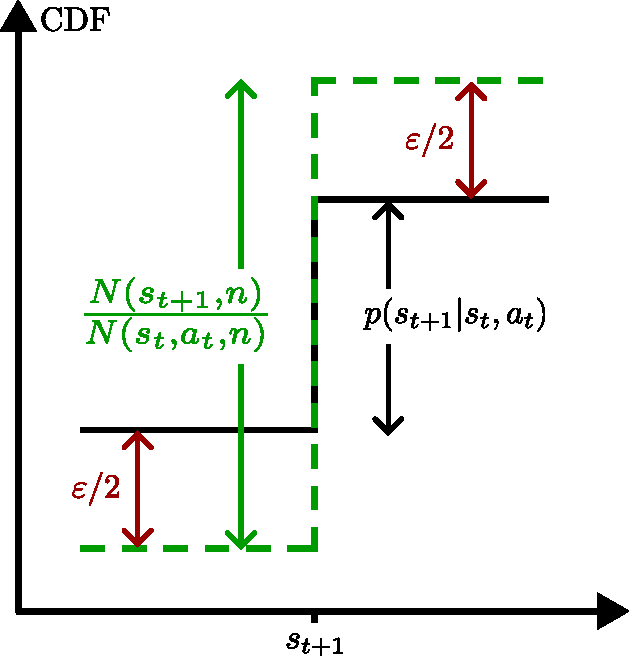
\includegraphics[scale=0.6]{figures/ch4/dkw_diagram.pdf}
        \caption[Bounding the empirical transition probabilities to the true transition probabilities.]{Bounding the empirical transition probabilities to the true transition probabilities. The true cdf is shown as a solid black line, the empirical cdf is shown as a dashed green line, and a worst case error of $\varepsilon/2$, using Theorem \ref{thrm:dkw_inequality}, is shown in red. The probability mass of $p(s_{t+1}|s_t,a_t)$ and empirical probability mass of $\frac{N(s_{t+1},n)}{N(s_t,a_t,n)}$ is also indicated to demonstrate how the constructed distribution gives Corollary \ref{cor:bound_transition_distribution}.}
        \label{fig:dkw_diag}
    \end{figure}
    %
    \begin{corollary} \label{cor:bound_transition_distribution}
        Consider any Boltzmann MCTS process. For all $(s_t,a_t)\in\cl{S}\times\cl{A}$ and for all $\varepsilon >0$ we have:
        \begin{align}
            \Pr\left(\max_{s_{t+1}\in\suc{s_t}{a_t}}\left| \frac{N(s_{t+1},n)}{N(s_t,a_t,n)} - p(s_{t+1}|s_t,a_t) \right| > \varepsilon \right) \leq 2 \exp\left(-\frac{1}{2}\varepsilon^2 N(s_t,a_t) \right).
        \end{align}
    \end{corollary}
    \begin{proofoutline}
        By considering some arbitrary ordering over the successor states in $\suc{s_t}{a_t}$ and applying Theorem \ref{thrm:dkw_inequality}, replacing $\varepsilon$ by $\varepsilon/2$, the result follows.

        To see why the factor of $1/2$ is needed, consider Figure \ref{fig:dkw_diag}. Because the distribution is discrete, the cumulative distribution function is a (piecewise constant) step function. As Theorem \ref{thrm:dkw_inequality} bounds the maximum difference between the empirical and true cumulative distribution functions, the factor of $1/2$ is needed to account for the error before and after each $s_{t+1}$ in the worst case.
    \end{proofoutline}









    






        


    Now that Corollary \ref{cor:bound_transition_distribution} can be used to bound  the empirical transition distribution to the true transition distribution,  a general purpose concentration inequality for Q-values can be proved for use in later proofs.
    
    \begin{lemma} \label{lem:stochastic_step}
        Consider any Boltzmann MCTS process, and some state action pair $(s_t,a_t)\in\cl{S}\times\cl{A}$. Let $\dot{V}^{N(s,n)}(s):\cl{S}\rightarrow \bb{R}$, $\dot{V}^*(s):\cl{S}\rightarrow \bb{R}$ be some estimated and optimal value functions respectively and suppose that for all $s_{t+1}\in\suc{s_t}{a_t}$ that there is some $C_{s_{t+1}}, k_{s_{t+1}}>0$ such that for all $\varepsilon_0 >0$:
        \begin{align}
            \Pr\left(\left| \dot{V}^{N(s_{t+1})}(s_{t+1}) - \dot{V}^*(s_{t+1}) \right| > \varepsilon_0 \right) \leq C_{s_{t+1}}\exp(-k_{s_{t+1}}\varepsilon_0^2 N(s')).
        \end{align}
        
        If the optimal and estimated Q-values are defined as follows: 
        \begin{align}
            \dot{Q}^*(s,a)&=R(s,a)+\bb{E}_{s'\sim p(\cdot|s,a)}\left[\dot{V}^*(s')\right], \\
            \dot{Q}^{N(s,a,n)}(s,a)&=R(s,a)+\sum_{s'\in\suc{s}{a}} \left[
                \frac{N(s',n)}{N(s,a,n)} \dot{V}^{N(s',n)}(s')\right].
        \end{align}
        
        Then there exists some $C,k>0$, for all $\varepsilon>0$ such that:
        \begin{align}
            \Pr\left(\left| \dot{Q}^{N(s,a,n)}(s,a) - \dot{Q}^*(s,a) \right| > \varepsilon \right) \leq C\exp(-k\varepsilon^2 N(s,a,n)).
        \end{align}
    \end{lemma}
    
    \begin{proof}
        By the assumed bounds, Lemma \ref{lem:union_bound} and Lemma \ref{lem:s_to_sa}, there is some $C_1,k_1>0$, such that for any $\varepsilon_1 >0$:
        \begin{align}
            \Pr\left(\forall s_{t+1}. \left|\dot{V}^{N(s_{t+1})}(s_{t+1})-\dot{V}^*(s_{t+1}) \right| \leq \varepsilon_1 \right) > 1-C_1\exp(-k_1\varepsilon_1^2 N(s_t,a_t,n)). \label{local:one}
        \end{align}

        And recall that for any $p(s_{t+1}|s_t,a_t) > \varepsilon_2>0$, using Corollary \ref{cor:bound_transition_distribution} that:
        \begin{align}
            \Pr\left(\max_{s_{t+1}\in\suc{s_t}{a_t}} 
                \left| \frac{N(s_{t+1},n)}{N(s_t,a_t,n)} - p(s_{t+1}|s_t,a_t) \right| 
                \leq \varepsilon_2 \right) 
                    > 1 - 2 \exp\left(-\frac{1}{2}\varepsilon_2^2 N(s_t,a_t,n) \right). \label{local:two}
        \end{align}
        
        If the events in Inequalities (\ref{local:one}) and (\ref{local:two}) hold, then the following inequalities must also hold:
        \begin{align}
            \dot{V}^*(s_{t+1})- \varepsilon_1 
                &\leq \dot{V}^{N_n(s_{t+1},n)}(s_{t+1}) 
                \leq \dot{V}^*(s_{t+1})+ \varepsilon_1 \\
            p(s_{t+1}|s_t,a_t) - \varepsilon_2 
                &\leq \frac{N(s_{t+1},n)}{N(s_t,a_t,n)} 
                \leq p(s_{t+1}|s_t,a_t) + \varepsilon_2.
        \end{align} 
        
        The upper bounds on $\dot{V}^{N_n(s_{t+1},n)}(s_{t+1})$ and $N(s_{t+1},n)/N(s_t,a_t,n)$ can be used to obtain an upper bound on $\dot{Q}^{N(s_t,a_t,n)}(s_t,a_t)$: 
        \begin{align}
            &\dot{Q}^{N(s_t,a_t,n)}(s_t,a_t) \\
                =& R(s_t,a_t) 
                    + \sum_{s_{t+1}\in\suc{s_t}{a_t}}\frac{N(s_{t+1},n)}{N(s_t,a_t,n)} 
                        \dot{V}^{N(s_{t+1},n)}(s_{t+1}) \\
                \leq& R(s_t,a_t) 
                    + \sum_{s_{t+1}\in\suc{s_t}{a_t}}(p(s_{t+1}|s_t,a_t)+\varepsilon_2)
                        (\dot{V}^*(s_{t+1})+\varepsilon_1) \\
                =& R(s_t,a_t) 
                    + \bb{E}_{s_{t+1}\sim p(\cdot|s_t,a_t)}[\dot{V}^*(s_{t+1})] 
                    + \varepsilon_1 
                    + \varepsilon_2\sum_{s_{t+1}\in\suc{s_t}{a_t}} \dot{V}^*(s_{t+1}) 
                    + \varepsilon_1 \varepsilon_2 \\
                \leq& R(s_t,a_t) 
                    + \bb{E}_{s_{t+1}\sim p(\cdot|s_t,a_t)}[\dot{V}^*(s_{t+1})] 
                    + \varepsilon_2\left|\sum_{s_{t+1}\in\suc{s_t}{a_t}} \dot{V}^*(s_{t+1})\right| 
                    + \varepsilon_1 + \varepsilon_1 \varepsilon_2 \\
                =& \dot{Q}^*(s_t,a_t) 
                    + \varepsilon_2\left|\sum_{s_{t+1}\in\suc{s_t}{a_t}} \dot{V}^*(s_{t+1})\right| 
                    + \varepsilon_1 
                    + \varepsilon_1 \varepsilon_2.
        \end{align}
        
        Following the similar reasoning but using the lower bounds on $\dot{V}^{N_n(s_{t+1},n)}(s_{t+1})$ and $N(s_{t+1},n)/N(s_t,a_t,n)$ gives: \todo{There is some special cases when V is negative, having to use the other bound, but the upper and lower bound have a bit of leway which handles all four cases of using plus minus epsilon one and two.}
        \begin{align}
            \dot{Q}^{N(s_t,a_t,n)}(s_t,a_t) 
                &\geq \dot{Q}^*(s_t,a_t) 
                    - \varepsilon_2\left|\sum_{s_{t+1}\in\suc{s_t}{a_t}} \dot{V}^*(s_{t+1})\right| 
                    - \varepsilon_1 
                    - \varepsilon_1 \varepsilon_2.
        \end{align}
        
        Now given an arbitrary $\varepsilon >0$, recalling that $\varepsilon_1,\varepsilon_2>0$ were arbitrary, set $\varepsilon_1 = \varepsilon/3$ and $\varepsilon_2 = \min(\varepsilon/3, \varepsilon/3|\sum_{s_{t+1}} \dot{V}^*(s_{t+1})|)$ to give:
        %
        \begin{align}
            \dot{Q}^*(s_t,a_t) - \varepsilon \leq \dot{Q}^{N(s_t,a_t,n)}(s_t,a_t) \leq \dot{Q}^*(s_t,a_t) + \varepsilon.
        \end{align}
        
        Using Lemma \ref{lem:union_bound} liberally, there is some $C_2,C_3,k_2,k_3>0$ such that:
        \begin{align}
            &\Pr\left(\left| \dot{Q}^{N(s_t,a_t,n)}(s_t,a_t) - \dot{Q}^*(s_t,a_t) \right| \leq \varepsilon \right) \\
                >& \left(1-C_1\exp(-k_1\varepsilon_1^2 N(s_t,a_t,n))\right) 
                    \left(1-2\exp\left(-\frac{1}{2}\varepsilon_2^2 N(s_t,a_t,n) \right)\right) \\
                =& \left(1-C_2\exp(-k_2 \varepsilon^2 N(s_t,a_t,n) \right) 
                    \cdot \left(1-C_3\exp(-k_3 \varepsilon^2 N(s_t,a_t,n)\right) \\
                % =& 1 -C_2\exp(-k_2 \varepsilon^2 N(s_t,a_t,n)) -C_3\exp(-k_3 \varepsilon^2 N(s_t,a_t,n)) \notag \\
                %     &+ C_2C_3\exp(-(k_2+k_3)\varepsilon^2 N(s_t,a_t,n) ) \\
                >& 1 -C_2\exp(-k_2 \varepsilon^2 N(s_t,a_t,n)) -C_3\exp(-k_3 \varepsilon^2 N(s_t,a_t,n)).
        \end{align}
        
        Finally, by negating and setting $C=C_2+C_3$ and $k=\min(k_2,k_3)$ in Lemma \todo{ref} the result follows:
        \begin{align}
                \Pr\left(\left| \dot{Q}^{N(s_t,a_t,n)}(s_t,a_t) - \dot{Q}^*(s_t,a_t) \right| > \varepsilon \right) \leq C\exp(-k\varepsilon^2 N(s_t,a_t,n)).
        \end{align}
    \end{proof}















  
\subsection{MENTS results} \label{app:ments_results}

    This subsection provides results related to MENTS in the setting of that standard reinforcement learning objective. Concentration inequalities are given around the optimal soft values to start with, although this result is similar to soem of the results provided in \cite{ments} \todo{this is still provided to keep this thesis' proofs self contained. (although its not as we use lots of things like hoeffdings, and also use UCT style proofs prsumably later on.) We could say ``to keep the proofs compatible with the other results provided. Or we could just omit it and reference the MENTS paper...''} Afterwards, the concentration inequalities are combined with results about maximum entropy reinforcement learning \todo{ref the section where we did that} to provide bounds on the simple regret of MENTS, given constraints on the temperature.
    








    To prove the concentration inequality around the optimal soft values, start by showing an inductive step.

    
    \begin{lemma} \label{lem:ments_val_induction_step}
        Consider a MENTS process. Let $s_t\in\cl{S}$, with $1\leq t \leq H$ \todo{update for thtspp notation}. If for all $s_{t+1}\in\bigcup_{a\in\cl{A}}\suc{s_t}{a}$ there is some $C_{s_{t+1}},k_{s_{t+1}}>0$ for any $\varepsilon_{s_{t+1}}>0$:
        \begin{align}
            \Pr\left(\left| \mVments{N(s_{t+1},n)}(s_{t+1}) - V_{\sft}^*(s_{t+1}) \right| > \varepsilon_{s_{t+1}} \right) 
                &\leq C_{s_{t+1}}\exp\left( -k_{s_{t+1}}\varepsilon_{s_{t+1}}^2 N(s_{t+1},n) \right), 
        \end{align}
        then there is some $C,k>0$, for any $\varepsilon>0$:
        \begin{align}
            \Pr\left(\left| \mVments{N(s_{t},n)}(s_t) - V_{\sft}^*(s_{t}) \right| > \varepsilon \right) 
                &\leq C\exp\left( -k\varepsilon^2 N(s_{t},n) \right).
        \end{align}
    \end{lemma}
    
    \begin{proof}
        Given the assumptions and by Lemmas \ref{lem:stochastic_step}, \ref{lem:sa_to_s} and \ref{lem:union_bound}, there is some $C,k>0$ such that for any $\varepsilon>0$:
        \begin{align}
            \Pr\left(\forall a_t\in\cl{A}. \left|\mQments{N(s_t,a_t,n)}(s_t,a_t)-Q_{\sft}^*(s_t,a_t)\right|\leq \varepsilon\right) &> 1-C \exp(-k \varepsilon^2 N(s_t,n)).
        \end{align}
        
        So with probability at least $1-C \exp(-k \varepsilon^2 N(s_t,n))$, for any $a_t$, the following holds:
        \begin{align}
            Q_{\sft}^*(s_t,a_t) - \varepsilon \leq \mQments{N(s_t,a_t,n)}(s_t,a_t) \leq Q_{\sft}^*(s_t,a_t) + \varepsilon. 
        \end{align}
        
        Using the upper bound on $\mQments{N(s_t,a_t,n)}(s_t,a_t)$ in the soft backup equation for $\mVments{N(s_t,n)}(s_t)$ (Equation (\ref{appeq:soft_v_backup}) gives:
        \begin{align}
            \mVments{N(s_t,n)}(s_t) &= \alpha \log \sum_{a\in\cl{A}} 
                    \exp\left(\frac{\mQments{N(s_t,a_t,n)}(s_t,a_t)}{\alpha}\right) \\
                &\leq \alpha \log \sum_{a\in\cl{A}} \exp\left(\frac{Q_{\sft}^*(s_t,a_t)+\varepsilon}{\alpha}\right) \\
                &= \left[\alpha \log \sum_{a\in\cl{A}} \exp\left(\frac{Q_{\sft}^*(s_t,a_t)}{\alpha}\right)\right] 
                    + \varepsilon \\
                &= V_{\sft}^*(s_t) + \varepsilon,
        \end{align}
        noting that the \textit{softmax} function monotonically increases in its arguments. Then with similar reasoning using the lower bound on $\mQments{N(s_t,a_t,n)}(s_t,a_t)$ gives:
        \begin{align}
            \mVments{N(s_t,n)}(s_t) \geq V_{\sft}^*(s_t) - \varepsilon,
        \end{align}
        and hence:
        \begin{align}
            |\mVments{N(s_t,n)}(s_t)-V_{\sft}^*(s_t)| \leq \varepsilon.
        \end{align}
        
        This therefore shows: \todo{some comment about how if A implies B then pr(B) more than pr(A)}
        \begin{align}
            \Pr\left(\left|\mVments{N(s_t,n)}(s_t)-V_{\sft}^*(s_t)\right| \leq \varepsilon_1\right) > 1-C \exp(-k \varepsilon^2 N(s_t,n)),
        \end{align}
        and negating probabilities gives the result.
    \end{proof}









        
    
    Then completing the induction gives the concentration inequalities desired for any state that MENTS might visit.
    \begin{theorem} \label{thrm:ments_val_converge}
        Consider a MENTS process, let $s_t\in\cl{S}$ then there is some $C,k>0$ for any $\varepsilon>0$:
        \begin{align}
            \Pr\left(\left| \mVments{N(s_{t},n)}(s_{t}) - V_{\sft}^*(s_{t}) \right| > \varepsilon \right) 
                &\leq C\exp\left( -k\varepsilon^2 N(s_{t},n) \right).
        \end{align}
        Moreover, at the root node $s_0$:
        \begin{align}
            \Pr\left(\left| \mVments{N(s_{0},n)}(s_{0}) - V_{\sft}^*(s_{0}) \right| > \varepsilon \right) 
                &\leq C\exp\left( -k\varepsilon^2 n \right). \label{local:three}
        \end{align}
        And hence $\mVments{N(s_{t},n)}(s_{t}) \rap V_{\sft}^*(s_{t})$.
    \end{theorem}
    \begin{proof}
        Consider that the result holds for $t=H+1$, because $\mVments{N(s_{H+1},n)}(s_{H+1})=V_{\sft}^*(s_{H+1})=0$. Therefore the result holds for any $t=0,...,H+1$ by induction using Lemma \ref{lem:ments_val_induction_step}. Noting that $N(s_0)=n$ gives (\ref{local:three}). \todo{To see the convergence in probability, let }$n\rightarrow\infty$. \todo{Double check the H stuf is consistent with the thtspp and MDP defns}
    \end{proof}










    Provided MENTS's temperature parameter is set small enough, such that the optimal standard and soft values lead to identical recommendation policies \todo{ref the max entropy proof of this}, then MENTS is consistent and the expected simple regret tends to zero exponentially. This is shown in the following lemma.
        
    \begin{lemma} \label{lem:ments_imm_simple_regret}
        Consider a MENTS process with $\alphaments<\Delta_{\cl{M}}/3H\log |\cl{A}|$. \todo{Make sure replaced alpha with alphaments in ments theorems} Let $s_t\in\cl{S}$, with $1\leq t \leq H$ then there is some $C',k'>0$ such that:
        \begin{align}
            \bb{E} \sreg(s_{t},\mpsiments{n}) &\leq C'\exp\left( -k' N(s_{t},n) \right).
        \end{align}
    \end{lemma}
    \begin{proof}
        \todo{Why cant we just replace this with, the values converge in probability from the previous result, and then use that it means the recommendation policy converges in probability, and then use that to say simple regret go zero? The case where it doesnt work is if there is suboptimal soft value which equals the optimal soft value (which has no entropy), in this case, becase we need the value ESTIMATES to converge, not the optimal values, we need the temperature to be a bit stricter. I think}

        Let $a^*$ be the optimal action with respect to the soft values, so $a^*=\argmax_{a\in\cl{A}} Q_{\sft}^*(s_t,a)$. Then by Lemma \ref{lem:soft_standard_consistent_order} $a^*$ must also be the optimal action for the standard Q-value function $a^*=\argmax_{a\in\cl{A}} Q^*(s_t,a)$. By Theorem \ref{thrm:ments_val_converge} and Lemmas \ref{lem:stochastic_step} and \ref{lem:sa_to_s} there exists $C_1,k_1>0$ such that for all $\varepsilon_1>0$: \todo{reword this paragraph, its a bit meh}
        \begin{align}
            \Pr\left(\forall a_t\in\cl{A} \left|\mQments{N(s_t,a_t,n)}(s_t,a_t)-Q_{\sft}^*(s_t,a_t)\right|\leq \varepsilon_1\right) &> 1-C_1 \exp(-k_1 \varepsilon_1^2 N(s_t,n)).
        \end{align}
        
        Setting $\varepsilon_1=\Delta_{\cl{M}}/3H\log |\cl{A}|$ then gives with probability at least $1-C_1 \exp(-k_2N(s_t,n))$ (where $k_2=k_1\left(\frac{\Delta_{\cl{M}}}{3H\log|\cl{A}|}\right)^2$) that for all actions $a_t\in\cl{A}$:
        \begin{align}
            Q_{\sft}^*(s_t,a_t) - \Delta_{\cl{M}}/3 \leq \mQments{N(s_t,a_t,n)}(s_t,a_t) \leq Q_{\sft}^*(s_t,a_t) + \Delta_{\cl{M}}/3.
        \end{align}
        
        And hence, with probability at least $1-C_1 \exp(-k_2N(s_t,n))$, for all $a\in\cl{A}-\{a^*\}$ we have:
        \begin{align}
            \mQments{N(s_t,a,n)}(s_t,a)
                \leq& Q_{\sft}^*(s_t,a) + \Delta_{\cl{M}}/3 \\
                \leq& Q^*(s_t,a) + \alpha H\log |\cl{A}| + \Delta_{\cl{M}}/3 \\
                \leq& Q^*(s_t,a) + 2\Delta_{\cl{M}}/3 \\
                \leq& Q^*(s_t,a^*) - \Delta_{\cl{M}}/3 \\
                \leq& Q_{\sft}^*(s_t,a^*) - \Delta_{\cl{M}}/3 \\
                \leq& \mQments{N(s_t,a^*,n)}(s_t,a^*). \label{local:nine}
        \end{align}
        
        Where in the above, the first line holds from the upper bound on $\mQments{N(s_t,a_t,n)}(s_t,a_t)$; The second holds from maximising the standard return and entropy portions of the soft value separately (recall Inequality (\ref{appeq:softdiv}) in Lemma \ref{lem:soft_standard_consistent_order}); The third holds from the assumption on $\alpha$; The fourth holds from the definition of $\Delta_{\cl{M}}$ (also see Inequality (\ref{appeq:delta_diff})); The fifth holds from the optimal soft value being greater than the optimal standard value (Lemma \ref{lem:soft_geq_standard}); And the final line holds by using the lower bound on $\mQments{N(s_t,a_t,n)}(s_t,a_t)$ given above with $a_t=a^*$. 
        
        Negating the probability that (\ref{local:nine}) holds gives:
        \begin{align}
            \Pr\left(\exists a_t\in\cl{A}-\{a^*\}.\left( 
                \mQments{N(s_t,a)}(s_t,a) > \mQments{N(s_t,a^*,n)}(s_t,a^*)\right)\right)
                \leq C_1 \exp(-k_2N(s_t)).
        \end{align}
        
        The expected immediate regret can be bounded as follows:
        \begin{align}
            & \bb{E}\ireg(s_t,\mpsiments{n})  \\
                =& \sum_{a\in\cl{A}-\{a^*\}} 
                    \left(V^*(s_t)-Q^*(s_t,a)\right) \Pr\left(\mpsiments{n}(s_t) =a \right) \\
                =& \sum_{a\in\cl{A}-\{a^*\}} 
                    \left(V^*(s_t)-Q^*(s_t,a)\right) \Pr\left(a = \argmax_{a'} \mQments{N(s_t,a',n)}(s_t,a') \right) \\
                \leq& \sum_{a\in\cl{A}-\{a^*\}} 
                    \left(V^*(s_t)-Q^*(s_t,a)\right) \Pr\left(\mQments{N(s_t,a,n)}(s_t,a) > \mQments{N(s_t,a^*,n)}(s_t,a^*)  \right) \\
                \leq&  \sum_{a\in\cl{A}-\{a^*\}} 
                    \left(V^*(s_t)-Q^*(s_t,a)\right) C_1 \exp(-k_2N(s_t,n)),
        \end{align}
        where $k'=k_2$ and $C'=C_1\sum_{a\in\cl{A}-\{a^*\}} \left(V^*(s_t)-Q^*(s_t,a)\right)$. Finally, using \todo{ref lemma} gives the result.
    \end{proof}









    
    In consequence to Lemma \ref{lem:ments_imm_simple_regret}, provided the sufficient conditions are met, MENTS is consistent and will converge to a simple regret of zero.
    \begin{theorem} \label{thrm:ments_simple_regret_converge}
        Consider a MENTS process with $\alphaments<\Delta_{\cl{M}}/3H\log |\cl{A}|$.\todo{H consistent with thtspp}  Let $s_t\in\cl{S}$, with $1\leq t \leq H$ \todo{H consistent with thtspp} then there is some $C',k'>0$ such that:
        \begin{align}
            \bb{E} \sreg(s_{t},\mpsiments{n}) &\leq C'\exp\left( -k' N(s_{t},n) \right).
        \end{align}
        And specifically, at the root node $s_0$:
        \begin{align}
            \bb{E} \sreg(s_{0},\mpsiments{n}) &\leq C'\exp\left( -k'n) \right).
        \end{align}
    \end{theorem}
    \begin{proof}
        This theorem holds as a consequence of Corollary \ref{cor:imm_to_full_simple_regret} and Lemma \ref{lem:ments_imm_simple_regret}, and noting that at the root node $N(s_0,n)=n$.
    \end{proof}









    \todo{this was a theorem in the main neurips paper. Need to decide how writing this up, so this may go}
    \todo{We} have now shown Theorem \ref{thrm:ments}:
    \begin{customthm}{3.2} 
        For any MDP $\cl{M}$, after running $n$ trials of the MENTS algorithm with $\alphaments \leq \Delta_{\cl{M}}/3H\log|\cl{A}|$, \todo{H consistent with thtspp} there exists constants $C,k>0$ such that: $\bb{E}[\sreg(s_0,\psi^n_{\textnormal{MENTS}})] \leq C\exp(-kn)$, where $\Delta_{\cl{M}}=\min \{Q^*(s,a,t)-Q^*(s,a',t)\vert Q^*(s,a,t) \neq Q^*(s,a',t),s\in\cl{S}, a,a'\in\cl{A},t\in\bb{N}\}$.
    \end{customthm}
    \begin{proof}
        This is part of Theorem \ref{thrm:ments_simple_regret_converge}.
    \end{proof}











    \todo{Want to change this result (below) to be, for any temperature alpha, there is some MDP that MENTS is not consistent. Then for theory story it can be that there is always a way to set params in DENTS that it will converge, but for MENTS the parameters depends on the MDP. The MDP to do this has one initial choice, with a reward of one, and then the other option is an entropy chain again, where the length is long enough such that MENTS will chose the entropy chain option.}



    \begin{figure}
        \centering
        
\includegraphics[width=0.4\textwidth]{figures/todo.jpg}
        \caption{\todo{Make fig and write caption for the MDP for the new proof.}}
        \label{fig:ments_not_consistent_env}
    \end{figure}


        
    \begin{customprop}{3.1}
        \todo{Adapt this argument, which is just c and p from the neurips appendix}
        There exists an MDP $\cl{M}$ and temperature $\alpha$ such that $\bb{E}[\sreg(s_0,\mpsiments{n})] \not\to 0$ as $n\to\infty$. That is, MENTS is not consistent.
    \end{customprop}
    
    \begin{proof}
        \todo{Adapt this argument, which is just c and p from the neurips appendix}
        We give a proof by construction. Recall the modified 10-chain problem, with $R_f=1/2$ in Figure \ref{fig:dchain_illustration_tres}, and consider a MENTS process (i.e. running MENTS) with a temperature $\alphaments=1$ for $n$ trials. By considering the optimal soft Bellman equations (\ref{eq:v_soft_bellman}) and (\ref{eq:q_soft_bellman}), one can verify that $Q_{\sft}^*(1,2)=0.9$ and $Q_{\sft}^*(1,1)=\log\left(\exp(1/2)+\sum_{i=0}^8\exp(i/10)\right)\approx 2.74$. 
        
        Theorem \ref{thrm:ments_val_converge}, Lemma \ref{lem:stochastic_step} and Lemma \ref{lem:sa_to_s} implies that there is some $C,k>0$ for any $\varepsilon > 0$:
        \begin{align}
            \Pr\left(\left| \mQments{N(1,1,n)}(1,1) - Q_{\sft}^*(1,1)\right| > \varepsilon \right) \leq C\exp(-k\varepsilon^2 N(1,n)) = C\exp(-k\varepsilon^2 n).
        \end{align}
        
        Letting $\varepsilon=1$ and using $Q_{\sft}^*(1,1)>5/2$ gives:
        \begin{align}
            \Pr\left(\mQments{N(1,1,n)}(1,1) < 3/2 \right) 
                \leq& \Pr\left(\left| \mQments{N(1,1,n)}(1,1) - Q_{\sft}^*(1,1)\right| > 1 \right) \\
                \leq& C\exp(-kn).
        \end{align}
        
        And hence:
        \begin{align}
            \Pr(\mpsidents{n}(1)=1) > 1 - C\exp(-kn)
        \end{align}
        
        Consider that the best simple regret an agent can achieve after selecting action 1 from the starting state is $1/10$. Let $M=\log(2C)/k$, so that $C\exp(-kM)=1/2$. Then, for all $n>M$ we have $\Pr(\psi^n_{\text{MENTS}}(1)=1)> 1/2$, and hence:
        \begin{align}
            \bb{E}\sreg(1,\mpsiments{n}) &> \frac{1}{10} \cdot \Pr(\psi^n_{\text{MENTS}}(1)=1) \\
                &> \frac{1}{20}.
        \end{align}
        Thus $\bb{E}\sreg(1,\mpsidents{n})\not\rightarrow 0$.
    \end{proof}






















    
    Finally for the MENTS proofs, an MDP can be constructed such that for any setting of $\alphaments$ MENTS will either not be consistent, or, will take exponentially long in the size of the state space of the MDP. This MDP is the \todo{whatever call the entropy trap env} first seen in \todo{ref to toy envs section figure}, where this phenominon was demonstrated empirically \todo{ref to graph in toy envs section}. This figure is repeated in Figure \ref{fig:adapted_chain} \todo{for ease of reading}.



    \begin{figure}
        \centering
        
\includegraphics[width=0.8\textwidth]{figures/todo.jpg}
        \caption{\todo{haven't edited this from the neurips paper, need to reproduce the fig and comment with the new notation} An illustration of the \textit{adapted-chain problem}, where 1 is the starting state, all transitions are deterministic and values next to states represents the reward for arriving in that state. The MDP is split into two sections, firstly, the UCT gauntlet refers to the D-chain part of the MDP, which is difficult for UCT algorithms, and secondly, the entropy trap, where the agent has to chose between states $E$ and $F$. The entropy trap consists of two chains of $K$ states, all of which give a reward of $0$ for visiting, but allows an agent to follow a policy with up to $\log(2)K$ entropy. So the optimal values for $E$ and $F$ are $V_{\sft}^*(E)=\log(2)K$ and $V_{\sft}^*(F)=1$ respectively.}
        \label{fig:adapted_chain}
    \end{figure}
    
    
    
    \begin{theorem} \label{thrm:ments_bad_mdp}
        Consider a MENTS process with arbitrary temperature $\alphaments$. There exists and MDP such that for any $\alphaments$ that MENTS is either not consistent, or requires an exponential number of trials in the size of the state space. More precisely, either $\mathbb{E}\sreg(s_0,\mpsiments{n})\not\rightarrow 0$ or $\mathbb{E}\sreg(1,\mpsiments{n}) \geq c(1 - \frac{n}{k^{|\cl{S}|}})$, which implies that $\mathbb{E}\sreg(s_0,\psi^n_{MENTS})>0$ for $n<k^{|\cl{S}|}$. 
    \end{theorem}
    
    \begin{proofoutline}
        \todo{remember this one was written in a bit of a rush, so probably want to make it a little clearer. Also need to make it consistent with the states and actions notation} 

        \todo{Also a bunch of N(s) instead of N(s,n) in the proof that need to be fixed}

        Proof is by construction. Consider the adapted-chain MDP \todo{update name for name change?} defined in Figure \ref{fig:adapted_chain}, which is parameterised by $D$ the length of the UCT gauntlet, and $K$, half the number of states in the entropy trap. To prove the claim, two cases need to be considered: when the temperature is sufficiently high for MENTS to get `caught' in the entropy trap when it is inconsistent; and, when the temperature is lower than this threshold.
        
        Case 1: $\alphaments>\frac{1}{\log(2)K}$ (MENTS gets caught by the entropy trap).
        
        If $\alphaments>\frac{1}{\log(2)K}$, the soft value of E is greater than one for any policy over the actions, and $\phi$ is a uniform policy (note that because there are no MDP rewards after $E$, $\phi$ is both the initial policy for MENTS and the optimal soft policy \todo{only for the entropy trap section}): 
        \begin{align}
                V_{\sft}^*(E) & = 0 + \alphaments \cdot \mathcal{H}(\phi) \\
                    & = \alphaments \cdot \log(2)  K \\
                    & > 1 \\
                    & = V_{\sft}^*(F).
        \end{align}
        
        Hence the optimal soft values (which MENTS converges to) will recommend going to state $E$ and gathering $0$ reward. Hence in this case the simple regret will converge to $1$ as the optimal value is $V^*(1)=1$. That is $\mathbb{E}\sreg(1,\mpsiments{n}) \rightarrow 1 > 0$.
        
        Case 2: $\alpha\leq\frac{1}{\log(2)K}$ \todo{asnother comment on this case, or remove comment from other case}
        
        In this case it is argued that with a low $\alphaments$ that MENTS will only have a low probability of ever hitting state $D$, that is, it requires a lot of trials to garuntee that at least one trial has reached state $D$, which is necessary to get the reward of $1$ (and simple regret of $0$).
        
        First consider the composed and simplified soft backup on the adapted-chain problem for any $0<i<D$ to get:
        \begin{align}
                \mVments{N(i,n)}(i) & = \alpha \log\left( \frac{1}{\alpha} 
                    \left( \frac{D-i}{D} + \mVments{N(i+1,n)}(i+1) \right)\right) \\
                & \leq \max\left(\frac{D-i}{D},\mVments{N(i+1,n)}(i+1)\right) + \alpha\log(2) \label{mbm:one} \\
                & \leq \max\left(\frac{D-i}{D},\mVments{N(i+1,n)}(i+1)\right) + \frac{1}{K}
        \end{align}
        
        where inequality (\ref{mbm:one}) used the property of log-sum-exp that $\alpha \log \sum_{i=1}^\ell \exp (x_i/\alpha) \leq \max_i (x_i) + \alpha \log(\ell)$. Assume that $K \geq D$ and $\mVments{N(D)}(D)=0$ (it will be checked that these assumptions are valid later). Then, by induction, it holds that $\mVments{N(i)}(i)\leq \frac{D-(i-1)}{D}$:
        \begin{align}
            \mVments{N(i)}(i) 
            & \leq \max\left(\frac{D-i}{D},\mVments{N(i+1)}(i+1)\right) + \frac{\log(2)}{\log(K)} \\
            & \leq \frac{D-i}{D} + \frac{1}{K} \\
            & \leq \frac{D-i}{D} + \frac{1}{D} \\
            & = \frac{D-(i-1)}{D}.
        \end{align}
        %
        \todo{first line uses induction hypothesis, value at i plus one less than D-i/D.}
        
        Now let the event $Y(n)$ be that MENTS visits state $D$ in its $n$th trial. Again assuming that $\mVments{N(D,n)}(D)=0$, the probability of this event occuring is less than $2^{-D}$. Because given this assumption it has just been shown that $\mVments{N(i+1,n)}(i+1)\leq \frac{D-i}{D} = \mVments{N(G_{i},n)}(G_{i})$, \todo{we are considering the choice between Gi and i plus 1 from state i here, which isn't too clear right now} as there are only two actions and taking action $a_R$ to continue down the chain has a lower soft value estimate, it must be that $\mpiments{n}(a_R|i) < \frac{1}{2}$, and as such, it must be that $\Pr\left(Y(n) \middle| \mVments{N(D,n)}(D)=0\right) < \frac{1}{2^D}$. 
         
        Then let $Z(n)=\neg \bigcup_{j=1}^n Y(j)$ be the event that no trial of MENTS has visited state $D$ in any of the first $n$ trials. And note that $Z(n)$ implies that $\mVments{N(D,n)}(D)=0$: \todo{probably aught to say somewhere in the proofs section that all the initialisations are set to zero, and the theory is to analyse the algorithms by itself, without any informative prior knowledge of the mdp}
        \begin{align}
            \Pr(Z(n)) 
                &= \Pr\left(Z(n) \cap \mVments{N(D,n)}(D)=0\right) \\
                &= \Pr\left(\neg Y(n) \cap Z(n-1) \cap \mVments{N(D,n)}(D) = 0  \right) \\
                &= \Pr\left(\neg Y(n) \middle| Z(n-1) \cap \mVments{N(D,n)}(D) = 0 \right) 
                    \Pr\left( Z(n-1) \cap \mVments{N(D,n)}(D) = 0 \right) \\
                &\geq (1-2^{-D}) \Pr\left( Z(n-1) \cap \mVments{N(D,n)}(D) = 0 \right) \\
                &= ... \\
                &\geq (1-2^{-D})^n \Pr\left( Z(0) \cap \mVments{N(D)}(D)=0\right) \\
                &= (1-2^{-D})^n \\
                &\geq 1-n2^{-D},
        \end{align}
        where the penultimate line used $\Pr\left( Z(0) \cap \left(\mVments{N(D)}(D)=0\right)\right)=1$, as $Z(0)$ and $\mVments{N(D,n)}(D)=0$ are vacuously true at the start of running the algorithm, and in the final line used Bernoulli's inequality \todo{ref}.
        
        Informally, $Z(n)$ implies that $V^{\mpsiments{n}}(1) \leq \frac{9}{10}$, as no trial has even reached $D$ to be able to reach the reward of $1$ from $F$. And hence the expected simple regret in this environment of MENTS can be bounded below as follows:
        \begin{align}
            \mathbb{E}\sreg(1,\psi^n_{\text{MENTS}}) 
                & \geq \left(1-\frac{9}{10}\right) \Pr(Z(n)) \\
                & \geq \frac{1}{10} \left( 1-n2^{-D} \right).
        \end{align}
        
        Finally, setting $K=D$, so that $|\cl{S}|=4D+3<5D$ for $D\in\bb{N}$ \todo{D more than 1} and so $D=\frac{|\cl{S}|-3}{4}>\frac{|S|}{5}$. Substituting this into the above inequality gives $\mathbb{E}\sreg(1,\mpsiments{n}) \geq 1 - \frac{n}{\sqrt[5]{2}^{|S|}}$, which is greater than $0$ for $n < \sqrt[5]{2}^{|S|}$. That is $c=\frac{1}{10}$ and $k=\sqrt[5]{2}$.
    \end{proofoutline}


    \todo{Some note about how DENTS can handle this case by using entropy and then ignoring it for the recommendations. Moreover, by allowing the entropy temperature (beta) to be decayed, allows the entropy trap estimates to correctly converge to the correct value of zero, and could handle a case where there is something more complex than a single state with a reward of one when not taking the entropy trap.}

    \todo{Additionally, note that because the proofs for convergence for DENTS have constraints on parameters (or no constraints on params) that even on this case it will converge to the correct result.}








\subsection{DENTS results} \label{appsec:dents_proofs}

    \todo{This is mostly the exponential bound stuff, so can also probably be appendix stuff}

    This subsection provides theoretical results that give exponential convergence of DENTS value estimates and simple regret. \todo{Some note on no constraints necessary on the parameters of DENTS?} 







    \begin{lemma} \label{lem:dents_val_induction_step}
        \todo{maybe should do directly from the Q values? Also same for the ments one?}
        Consider a DENTS process. Let $s_t\in\cl{S}$, with $1\leq t \leq H$. \todo{make H consistent with thtspp} If for all $s_{t+1}\in\bigcup_{a\in\cl{A}}\suc{s_t}{a}$ there is some $C_{s_{t+1}},k_{s_{t+1}}>0$ such that for any $\varepsilon_{s_{t+1}}>0$:
        \begin{align}
            \Pr\left(\left| \mVdents{N(s_{t+1},n)}(s_{t+1}) - V^*(s_{t+1}) \right| > \varepsilon_{s_{t+1}} \right) 
                &\leq C_{s_{t+1}}\exp\left( -k_{s_{t+1}}\varepsilon_{s_{t+1}}^2 N(s_{t+1},n) \right), 
        \end{align}
        then there is some $C,k>0$, for any $\varepsilon>0$:
        \begin{align}
            \Pr\left(\left| \mVdents{N(s_{t},n)}(s_{t}) - V^*(s_t) \right| > \varepsilon \right) 
                &\leq C\exp\left( -k\varepsilon^2 N(s_{t},n) \right).
        \end{align}
    \end{lemma}
    \begin{proof}
        Given the assumptions and by Lemmas \ref{lem:stochastic_step}, \ref{lem:union_bound} and \ref{lem:sa_to_s}, for some $C,k>0$ and for any $\varepsilon_1>0$:
        \begin{align}
            \Pr\left(\forall a_t\in\cl{A}. \left|\mQdents{N(s_t,a_t,n)}(s_t,a_t)-Q^*(s_t,a_t)\right|
                \leq \varepsilon_1\right) &> 1-C \exp(-k \varepsilon_1^2 N(s_t)).
        \end{align}
        
        Let $\varepsilon >0$, and set $\varepsilon_1 = \min(\varepsilon,\Delta_{\cl{M}}/2)$. So with probability at least $1-C_1 \exp(-k_1 \varepsilon_1^2 N(s_t,n))$ for any $a_t$ it must be that:
        \begin{align}
            Q^*(s_t,a_t) - \varepsilon_1 \leq \mQdents{N(s_t,a_t,n)}(s_t,a_t) &\leq Q^*(s_t,a_t) + \varepsilon_1. 
                \label{local:ten}
        \end{align}
        
        Let $a^*=\max_{a\in\cl{A}} Q^*(s_t,a)$. Using $\varepsilon_1 \leq \Delta_{\cl{M}}/2$ in (\ref{local:ten}), then for any $a\in\cl{A}-\{ a^*\}$:
        \begin{align}
            \mQdents{N(s_t,a,n)}(s_t,a) \leq& Q^*(s_t,a) + \Delta_{\cl{M}}/2 \\
                \leq& Q^*(s_t,a^*) - \Delta_{\cl{M}}/2 \\
                \leq& \mQdents{N(s_t,a^*,n)}(s_t,a^*),
        \end{align}
        and hence $\argmax_{a\in\cl{A}} \mQdents{N(s_t,a,n)}(s_t,a) = a^*$. As a consequence:
        \begin{align}
            \mVdents{N(s_t,n)}(s_t) &= \max_a \mQdents{N(s_t,a,n)}(s_t,a) = \mQdents{N(s_t,a^*,n)}(s_t,a^*). 
                \label{local:editing_one}
        \end{align}
        
        Then using (\ref{local:ten}) with $a_t=a^*$ (noting $V^*(s_t)=Q^*(s_t,a^*)$), using (\ref{local:editing_one}) and using $\varepsilon_1 \leq \varepsilon$ gives:
        \begin{align}
            V^*(s_t) - \varepsilon
                \leq& V^*(s_t) - \varepsilon_1 \\
                \leq& \mVdents{N(s_t,n)}(s_t) \\
                \leq& V^*(s_t) + \varepsilon_1 \\
                \leq& V^*(s_t) + \varepsilon. 
        \end{align}
        
        Hence:
        \begin{align}
            \Pr\left(\left|\mVdents{N(s_t,n)}(s_t)-V^*(s_t)\right| > \varepsilon\right) 
                &\leq C \exp(-k \varepsilon_1^2 N(s_t,n)) \\
                &\leq C \exp(-k \varepsilon^2 N(s_t,n)),
        \end{align}
        which is the result.
    \end{proof}












    
    
    Similarly to the MENTS section, Lemma \ref{lem:dents_val_induction_step} provides an inductive step, which is used in Theorem \ref{thrm:dents_val_converge} to show concentration inequalities at all states that DENTS visits.
        
    \begin{theorem} \label{thrm:dents_val_converge}
        Consider a DENTS process, let $s_t\in\cl{S}$ then there is some $C,k>0$ for any $\varepsilon>0$:
        \begin{align}
            \Pr\left(\left| \mVdents{N(s_{t},n)}(s_t) - V^*(s_{t}) \right| > \varepsilon \right) 
                &\leq C\exp\left( -k\varepsilon^2 N(s_{t},n) \right).
        \end{align}
        Moreover, at the root node $s_0$:
        \begin{align}
            \Pr\left(\left| \mVdents{N(s_{0},n)}(s_0) - V^*(s_0) \right| > \varepsilon \right) 
                &\leq C\exp\left( -k\varepsilon^2 n \right). \label{local:four}
        \end{align}
    \end{theorem}
    \begin{proof}
        The result holds for $t=H+1$ \todo{consistent with thtspp. SHOULD JUST CTRL-F THIS and sort all of these out at once.} because $\mVdents{N(s_{H+1})}(s_{H+1})=V^*(s_{H+1})=0$. \todo{might be an off by one error here dep on how defined H, check over this whole paragraph.} Hence the result holds for all $t=1,...,H+1$ by induction using Lemma \ref{lem:dents_val_induction_step}. Noting that $N(s_0)=n$ gives (\ref{local:four}).
    \end{proof}









    \todo{is this just repeated? Can we merge two of the proofs?}

    Again, the concentration inequalities are used to show that the simple regret tends to zero exponentially, and therefore that DENTS will be exponentially likely in the number of visits to recommend the optimal standard action at every node.
        
    \begin{lemma} \label{lem:dents_imm_simple_regret}
        Consider a DENTS process. Let $s_t\in\cl{S}$, with $1\leq t \leq H$ \todo{defn with thtspp for H agen} then there is some $C',k'>0$ such that:
        \begin{align}
            \bb{E} \ireg(s_{t},\mpsidents{n}) &\leq C'\exp\left( -k' N(s_{t},n) \right).
        \end{align}
    \end{lemma}
    \begin{proof}
        Let $a^*$ be the locally optimal standard action, so $a^*=\argmax_{a\in\cl{A}} Q^*(s_t,a)$. By Theorem \ref{thrm:dents_val_converge} and Lemmas \ref{lem:stochastic_step} and \ref{lem:sa_to_s} there exists $C_1,k_1>0$ such that for all $\varepsilon_1>0$:
        \begin{align}
            \Pr\left(\forall a_t\in\cl{A}. \left|\mQdents{N(s_t,a_t,n)}(s_t,a_t)-Q^*(s_t,a_t)\right|\leq \varepsilon_1\right) &> 1-C_1 \exp(-k_1 \varepsilon_1^2 N(s_t,n)).
        \end{align}
        
        Setting $\varepsilon_1=\Delta_{\cl{M}}/2$ then gives with probability $1-C_1 \exp(-k_2N(s_t,n))$ (where $k_2=k_1\Delta_{\cl{M}}/2$) for all actions $a\in\cl{A}$ that:
        \begin{align}
            Q^*(s_t,a) - \Delta_{\cl{M}}/2 \leq \mQdents{N(s_t,a,n)}(s_t,a) \leq Q^*(s_t,a) + \Delta_{\cl{M}}/2.
        \end{align}
        
        And hence, with probability $1-C_1 \exp(-k_2N(s_t))$, for all $a_t\in\cl{A}-\{a^*\}$ it must be that:
        \begin{align}
            \mQdents{N(s_t,a,n)}(s_t,a_t)
                \leq& Q^*(s_t,a_t) + \Delta_{\cl{M}}/2 \\
                \leq& Q^*(s_t,a^*) - \Delta_{\cl{M}}/2 \\
                \leq& \mQdents{N(s_t,a^*,n)}(s_t,a^*). \label{local:eleven}
        \end{align}
        
        Negating the probability of (\ref{local:eleven}) then gives:
        \begin{align}
            \Pr\left(\mQdents{N(s_t,a,n)}(s_t,a) > \mQdents{N(s_t,a^*,n)}(s_t,a^*)\right) \leq C_1 \exp(-k_2N(s_t,n))
        \end{align}
        
        Finally, the bound on the expected immediate regret follows:
        \begin{align}
            & \bb{E}\ireg(s_t,\mpsidents{n})  \\
                =& \sum_{a\in\cl{A}-\{a^*\}} 
                    \left(V^*(s_t)-Q^*(s_t,a)\right) \Pr\left(\mpsidents{n}(s_t) =a \right) \\
                =& \sum_{a\in\cl{A}-\{a^*\}} 
                    \left(V^*(s_t)-Q^*(s_t,a)\right) \Pr\left(a = \argmax_{a'} \mQdents{N(s_t,a,n)}(s_t,a) \right) \\
                \leq& \sum_{a\in\cl{A}-\{a^*\}} 
                    \left(V^*(s_t)-Q^*(s_t,a)\right) 
                    \Pr\left(\mQdents{N(s_t,a,n)}(s_t,a) > \mQdents{N(s_t,a^*,n)}(s_t,a^*)  \right) \\
                \leq&  \sum_{a\in\cl{A}-\{a^*\}} 
                    \left(V^*(s_t)-Q^*(s_t,a)\right) C_1 \exp(-k_2N(s_t,n)),
        \end{align}
        and setting $k'=k_2$ and $C'=C_1\sum_{a\in\cl{A}-\{a^*\}} \left(V^*(s_t)-Q^*(s_t,a)\right)$ gives the result.
    \end{proof}











    
    Again similarly to before, by using Lemma \ref{lem:dents_imm_simple_regret}, the bound on the immediate simple regret can be converted to a bound on the simple regret.
        
    \begin{theorem} \label{thrm:dents_simple_regret_converge}
        Consider a DENTS process. Let $s_t\in\cl{S}$, with $1\leq t \leq H$ \todo{thtspp consistent agen} then there is some $C',k'>0$ such that:
        \begin{align}
            \bb{E} \sreg(s_{t},\mpsidents{n}) &\leq C'\exp\left( -k' N(s_{t},n) \right).
        \end{align}
        
        Moreover, at the root node $s_0$:
        \begin{align}
            \bb{E} \sreg(s_{0},\mpsidents{n}) &\leq C'\exp\left( -k'n \right). \label{local:five}
        \end{align}
    \end{theorem}
    \begin{proof}
        Theorem holds as a consequence of Corollary \ref{cor:imm_to_full_simple_regret} and Lemma \ref{lem:dents_imm_simple_regret}. To arrive at (\ref{local:five}) note that $N(s_0,n)=n$.
    \end{proof}














    Finally, Theorem \ref{thrm:dents} follows \todo{this was the neurips main paper theorem, changing how doing the main results bit} from the results that we have just shown.


    Finally, Theorem \ref{thrm:dents} hows as it is a subset of what has already been shown.
    \begin{customthm}{4.2}
        \todo{this was the neurips main paper theorem, only changed enough to get this compiling. Also need to change the results for correct conditions, dont think beta needs to be bounded actually}
        For any MDP $\cl{M}$, after running $n$ trials of the DENTS algorithm with a root node of $s_0$, if $\betadents$ is bounded above and $\betadents(m)\geq 0$ for all $m\in\bb{N}$, then there exists constants $C,k>0$ such that for all $\varepsilon>0$ it holds that
        $\bb{E}[\sreg(s_0,\mpsidents{n})] \leq C\exp(-kn)$, and also $\mVdents{N(s_0,n)}(s_0) \rap V^*(s_0)$ as $n\rightarrow\infty$.
    \end{customthm}
    \begin{proof}
        The simple regret bound follows immediately from Theorem \ref{thrm:dents_simple_regret_converge}. Using Theorem \ref{thrm:dents_val_converge} it holds that $\Pr\left(\left| \mVdents{N(s_{0},n)}(s_0) - V^*(s_0) \right| > \varepsilon \right) \leq C\exp\left( -k\varepsilon^2 n \right) \rightarrow 0$ as $n\rightarrow \infty$, and hence $\mVdents{N(s_{0},n)}(s_0)$ converges in probability to $V^*(s_0)$.
    \end{proof}
















    
\subsection{BTS results} \label{appsec:bts_proofs}

    Recall that the BTS process is a special case of the DENTS process, where the decay function is set to $\betadents(m)=0$. As such, all of the results for DENTS processes also hold for BTS processes, and specifically Theorem \ref{thrm:bts} \todo{neurips theorem} must hold.

    \todo{probably want to delete this and be more clear in the intro to the theory section that BTS is just a special case of DENTS mathematically. Also want to say that BTS does have a purpose in being a standalone algorithm when entropy isn't useful and so doing the second backup is useless. Commented out below is the main BTS theorem from the neurips paper}

    
    % \begin{customthm}{4.1}
    %     For any MDP $\cl{M}$, after running $n$ trials of the BTS algorithm with a root node of $s_0$, there exists constants $C,k>0$ such that for all $\varepsilon>0$ we have $\bb{E}[\reg(s_0,\psi^n_{\textnormal{BTS}})] \leq C\exp(-kn)$, and also $\Vt{s_0}{N(s_0)} \rap V^*(s_0)$ as $n\rightarrow\infty$.
    % \end{customthm}
    % \begin{proof}
    %     Follows from setting $\beta(m)=0$ and using Theorem \ref{thrm:dents}.
    % \end{proof}


















\subsection{Results for using average returns in Boltzmann MCTS processes} \label{sec:ar_proofs}

    \todo{SOME of this should be integrated into the main arguments I think}

    \todo{N(s) to N(s,n) stuff}

    In this section informal proof outlines for theoretical results for AR-BTS and AR-DENTS are given. To begin with define the average return $\bar{V}^{N(s)}(s)$ for a decision node at $s$, and recall the definition of $\bar{Q}^{N(s,a)}(s, a)$:

    \begin{align}
        \bar{V}^{N(s_t)+1}(s_t) &= \bar{V}^{N(s_t)}(s_t) + \frac{\bar{R}(s_t) - \bar{V}^{N(s_t)}(s_t)}{N(s_t) + 1},  \label{appeq:ar_v} \\
        \bar{Q}^{N(s_t,a_t)+1}(s_t, a_t) &= \bar{Q}^{N(s_t,a_t)}(s_t, a_t) 
            + \frac{\bar{R}(s_t,a_t) - \bar{Q}^{N(s_t,a_t)}(s_t, a_t)}{N(s_t, a_t) + 1},  \label{appeq:ar_q}
    \end{align}
    %
    where $\bar{R}(s_t)=\sum_{i=t}^H R(s_i,a_i)$ and $\bar{R}(s_t, a_t)=\sum_{i=t}^H R(s_i,a_i)$. Note that these average return values also satisfy the equations:
    %
    \begin{align}
        \bar{V}^{N(s_t)}(s_t) &= \sum_{a\in\cl{A}} \frac{N(s_t,a)}{N(s_t)} \bar{Q}^{N(s_t,a_t)}(s_t, a_t), \label{appeq:ar_v_rel} \\
        \bar{Q}^{N(s_t,a_t)}(s_t, a_t) 
            &= R(s_t,a_t) + \sum_{a\in\cl{A}} \frac{N(s')}{N(s_t,a_t)} \bar{V}^{N(s')}(s'). \label{appeq:ar_q_rel}
    \end{align}
    %
    \todo{should we do the rearrangement/working out for this?}










    \todo{Sufficiency for ar-bts to have temp tend to zero, but would need to change the theorem to say lower bound on temp rather than just fixed temp.}
    Firstly, it can be shown that using a non-decaying search temperature with AR-BTS is not guaranteed to recommend the optimal policy.
    
    \begin{figure}
        \centering
        
\includegraphics[width=0.7\textwidth]{figures/todo.jpg}
        \caption{\todo{Haven't touched this, need to reproduce from neurips paper}An MDP that AR-BTS will not converge to recommending the optimal policy on, for a large enough value of $D$.}
        \label{fig:ar_gen_mdp}
    \end{figure}

    \begin{customprop}{B.1}
        \todo{Haven't touched this, just c and p from neurips paper}

        For any $\alpha_{\textnormal{fix}}>0$, there is an MDP $\cl{M}$ such that AR-BTS with $\alpha(m)=\alpha_{\textnormal{fix}}$ is not consistent: $\bb{E}[\sreg(s_0,\psi^n_{\textnormal{AR-BTS}})] \not\to 0$ as $n\to\infty$. 
    \end{customprop}
    \begin{proofoutline}
        \todo{Haven't touched this, just c and p from neurips paper}

        Consider the MDP given in Figure \ref{fig:ar_gen_mdp}. We can show inductively that (as $n\rightarrow\infty$) the value of $\bb{E}\bar{V}^{N(k)}(k)\leq 2E^{D-k+1} < 2$, where $E=e^2/(1+e^2)$ for $2\leq k \leq D$. The inductive step is as follows:
        \begin{align}
            \bb{E}\bar{V}^{N(k)}(k) =& \frac{\exp\left(\bar{V}^{N(k+1)}(k+1)\right)}{1+\exp\left(\bar{V}^{N(k+1)}(k+1)\right)} \bb{E}\bar{V}^{N(k+1)}(k+1) 
                + \frac{1}{1+\exp\left(\bar{V}^{N(k+1)}(k+1)\right)} \cdot 0 \\
                \leq& E \cdot \bb{E} \bar{V}^{N(k+1)}(k+1) \\
                \leq& E \cdot 2E^{D-k} \\
                =& 2E^{D-k+1}.
        \end{align}

        where we know that $\exp\left(\bar{V}^{N(k+1)}(k+1)\right)/\left(1+\exp\left(\bar{V}^{N(k+1)}(k+1)\right)\right) < E$, because the function $e^x/(1+e^x)$ is monotonically increasing in $x$, and $\bar{V}^{N(k+1)}(k+1) < 2$. Hence, by choosing an integer $D$ such that $D-1 \geq \log(1/3) / \log(E)$, we have $\bb{E}\bar{V}^{N(2)}(2)=2E^{D-1}\leq 2/3 < 1 = \bb{E}\bar{Q}^{N(1,a_2)}(1,a_2)$. 

        A full proof should show that AR-BTS does indeed converge to these expected values, possibly through concentration bounds. 
        \todo{(was camera ready todo) Do the full proof, and show that AR-BTS converges to these value with non zero prob, hence the non zero simple regret.} 

        Hence, AR-BTS does not converge to a simple regret of zero, because the expected Q-values as $n\rightarrow\infty$ are $\bb{E}\bar{Q}^{N(1,a_2)}(1,a_2)=1$ and $\bb{E}\bar{Q}^{N(1,a_1)}(1,a_1)<2/3$, so AR-BTS would incorrectly recommend action $a_2$ from the root node. 
        \todo{(Was camera ready todo) Formally give the simple regret converges to something strictly greater than zero. Also can I even do that intersection to product equality? Doesn't that mean that they are independent. Are they independent?}
    \end{proofoutline}




    \todo{Say that AR-DENTS with beta not o(alpha) isn't consistent. Show that it essentially leads to a term of one times the entropy value, and so repeating the arguments that showed MENTS is inconsistent would show that AR-DENTS is inconsistent in this case. So this and the above AR-BTS results show that the conditions are necessary too.}

    \todo{Sufficiency for most visited stuff could also be done? Probably extending from these arguments, or saying that it would contradict these results.}










    \todo{This proof is re-written and improved on below, so this should be deleted.}
    \begin{lemma} \label{oldlem:inf_often_action_select}
        Let $\rho^k$ be an arbitrary policy, and let a search policy be $\pi^k(a)=(1-\lambda(k))\rho^k(a) + \lambda(k) / |\cl{A}|$, with $\lambda(k)=\min(1,\epsilon/\log(e+k))$, where $\epsilon\in(0,\infty)$. Let $a^k\sim \pi^k$, and let $M(a)$ be the number of times action $a$ was sampled out of $m$ samples, i.e. $M(a)=\sum_{i=1}^m \one[a^i=a]$. Then for all $a\in\cl{A}$ we have $M(a)\rightarrow\infty$ as $m\rightarrow \infty$.
    \end{lemma}
    \begin{proofoutline}
        This lemma restated means that our search policies will select all actions infinitely often. To show this, we argue by contradiction, and suppose that there is some $b\in\cl{A}$ such that after $\ell$ samples that $b$ is never sampled again. The probability of this happening at the $m$th sample is then:
        \begin{align}
            \Pr\left(\bigcap_{i=\ell}^m a^i \neq b \right)
                &= \prod_{i=\ell}^m \Pr(a^i \neq b) \\
                &\leq \prod_{i=\ell}^m \left( 1 - \frac{\epsilon}{|\cl{A}|\log(e+i)} \right) \\
                &\leq \left( 1 - \frac{\epsilon}{|\cl{A}|\log(e+m)} \right)^{m-\ell} \\
                &\rightarrow 0,
        \end{align}
        as $m\rightarrow\infty$. Which is a contradiction. 
    \end{proofoutline}







    \todo{This proof is re-written and improved on below, so this should be deleted.}
    \begin{customthm}{B.2} %\label{thrm:ar_bts}
        For any MDP $\cl{M}$, if $\alpha(m)\rightarrow 0$ as $m\rightarrow\infty$ then $\bb{E}[\sreg(s_0,\psi^n_{\textnormal{AR-BTS}})]\rightarrow 0$ as $n\rightarrow\infty$, where $n$ is the number of trials.
    \end{customthm}
    \begin{proofoutline}
        We can argue that average returns converge in probability by induction similar to the previous proofs. Suppose that $\bar{Q}^{N(s_t,a_t)}(s_t, a_t) \rap Q^*(s_t,a_t)$ as $N(s_t,a_t)\rightarrow\infty$. From Lemma \ref{lem:inf_often_action_select}, we know that if $N(s_t)\rightarrow\infty$, then $N(s_t,a_t)\rightarrow\infty$.

        All that remains to show that $\bar{V}^{N(s_t)}(s_t) \rap V^*(s_t)$ as $N(s_t)\rightarrow\infty$ is that $\frac{N(s_t,a)}{N(s_t)}\rightarrow \one[a=a^*]$. If that is true, then by considering Equation (\ref{appeq:ar_v_rel}), we can see that in the limit $\bar{V}^{N(s_t)}(s_t)$ tends to $\bar{Q}^{N(s_t,a*)}(s_t,a*)$. 
        \todo{(old cr todo)formally prove that the distribution and value converges. Will need some epsilons and use the equation referenced for the value. the distribution bit needs to show that eventually the samples are dominated by the greedy boltzmann policy, and not the exploration part}

        Intuitively we can see that $\frac{N(s_t,a)}{N(s_t)}\rightarrow \one[a=a^*]$ as the AR-BTS search policy converges to a greedy policy as $\alpha(m)\rightarrow 0$. 
        \todo{(old cr todo)technically only the rho bit does, shrugs}
    \end{proofoutline}










    \todo{Cut this one, also assumption is a bit off, and I think we're proving stuff correctly below in the additional section later}
    \begin{customthm}{B.3} 
        For any MDP $\cl{M}$, if $\alpha(m)\rightarrow 0$ and $\beta(m)\rightarrow 0$ as $m\rightarrow\infty$ then $\bb{E}[\sreg(s_0,\psi^n_{\textnormal{AR-DENTS}})]\rightarrow 0$ as $n\rightarrow\infty$, where $n$ is the number of trials.
    \end{customthm}
    \begin{proofoutline}
        Proof is similar to the proof for Theorem \ref{thrm:ar_bts}.
    \end{proofoutline}
    
    
    
    \todo{Probably delete this too}
    As a final note, using BTS or DENTS with a decaying search temperature $\alpha(m)$ will lead to a consistent algorithm, although they would not admit an exponential regret bound. Proofs would be nearly identical to Theorems \ref{thrm:ar_bts} and \ref{thrm:ar_dents}.










%%%%
% THEORY - Consistency Of Boltzmann MCTS Processes
%%%%

\subsection{Consistency Of Boltzmann MCTS Processes}
    


    \todo{Generally look into how to justify that we take limits in parts. Got the dominated convergence theorem from here: https://math.stackexchange.com/questions/15240/when-can-you-switch-the-order-of-limits/15296\#15296. Probably just leave the places where we do it as handwavy proof outlines}

    \todo{Which on that note, make sure we're using proof outline in this section, not proof}

    \todo{Generally clean up the writing here.}





    \todo{Make this the main section showing consistency of Boltzmann MCTS processes and under what conditions. Have the missing proofs written up on ipad.}
    
    \todo{Also write up the general steps from the ipad notes (which I think need a bit of correction.)}

    Because the search temperature is now decayed, \todo{we} need to show that the exploration term in the search policies leads to actions being sampled infinitely often.


    \todo{This lemma restated means that Boltzmann search policies will select all actions infinitely often.}
    \todo{Check the variables in this proof are consistent with the definitions of N(s,a,m) etc}

    \begin{lemma} \label{lem:inf_often_action_select}
        Let $\rho^m$ be an arbitrary policy, and the following policy: \todo{handle when epsilon is greater than one? I think its just let ell be large enough argument}
        \begin{align} 
            \pi^m(a)=(1-\lambda(m))\rho^m(a) + \lambda(m) \frac{1}{|\cl{A}|}, \label{appeq:ioas_policy}
        \end{align} 
        with $\lambda(m)=\min(1,\epsilon/\log(e+m))$, where $\epsilon\in(0,\infty)$. Let $a^m\sim \pi^m$ be the $m$th sampled action, and let $M(a,m)$ be the number of times action $a$ was selected in the first $m$ samples, i.e. $M(a,m)=\sum_{m=1}^m \one[a^m=a]$. Then for all $a\in\cl{A}$ we have $M(a,m)\raas\infty$ as $m\rightarrow \infty$.
    \end{lemma}
    \begin{proof}
        First consider that if $M(a,m)\not\rightarrow\infty$ then it is logically equivalent to say that there exists some $\ell$ such that from $a^\ell$ onwards that there is some action which is never sampled again. To prove the result, argue by contradiction, and suppose that there is some $\ell\in\bb{N}$ and $b\in\cl{A}$ such that:
        \begin{align}
            \Pr\left(\bigcap_{m=\ell}^\infty a^m \neq b\right) > 0. \label{appeq:ioas_contradict}
        \end{align}

        However, from the definition of equation (\ref{appeq:ioas_policy}) it must be that:
        \begin{align}
            \Pr\left(a^m = b\right) \geq \frac{\lambda(m)}{|\cl{A}|} = \frac{\epsilon}{|\cl{A}| \log(e+m)}.
        \end{align} 

        And so using this lower bound to work out the probability of never sampling action $b$ again after the first $\ell-1$ samples gives:
        \begin{align}
            \Pr\left(\bigcap_{m=\ell}^\infty a^m \neq b \right)
                &= \lim_{k\rightarrow\infty} \prod_{m=\ell}^k 
                    \Pr(a^m \neq b) \\
                &\leq \lim_{k\rightarrow\infty} \prod_{m=\ell}^k 
                    \left( 1 - \frac{\epsilon}{|\cl{A}|\log(e+k)} \right) \\
                &\leq \lim_{k\rightarrow\infty} 
                    \left( 1 - \frac{\epsilon}{|\cl{A}|\log(e+k)} \right)^{k-\ell} \label{appeq:ioas_one} \\
                &= 0, \label{appeq:ioas_two}
        \end{align}
        %
        which is in contradiction to inequality (\ref{appeq:ioas_contradict}) that was assumed. Inequality (\ref{appeq:ioas_one}) holds because the factors in the product are increasing with respect to $m$. To see why the final limit equality (\ref{appeq:ioas_two}) holds, consider the simpler function $f(x)=\left(1-1/\log(x)\right)^x$. Taking logarithms and applying L'Hopital's rule \todo{cite?} generously gives:
        \begin{align}
            \lim_{x\rightarrow \infty} \log f(x) 
            &= \lim_{x\rightarrow \infty} x \log\left(1-\frac{1}{\log(x)}\right) \\
            &= \lim_{x\rightarrow \infty} \frac{\log\left(1-\frac{1}{\log(x)}\right)}{x^{-1}} \\
            &= \lim_{x\rightarrow \infty} \frac{\frac{1}{x\log(x)(\log(x)-1)}}{-x^{-2}} \\
            &= \lim_{x\rightarrow \infty} \frac{-x}{\log(x)(\log(x)-1)} \\
            &= \lim_{x\rightarrow \infty} \frac{-x}{2\log(x)-1} \\
            &= \lim_{x\rightarrow \infty} \frac{-x}{2} \\
            &= -\infty.
        \end{align} 
        %
        And thus $\lim_{x\rightarrow\infty} f(x) = \lim_{y\rightarrow -\infty} e^{y} = 0$.

        \todo{cut this down maybe, its a little excessive showing all of the working out?}

        Hence, by contradiction, it must be the case that $\Pr(M(a,m)\not\rightarrow\infty) = 0$, or rather that $\Pr(M(a,m)\rightarrow\infty) = 1$ which is the desired result.
    \end{proof}
    %
    \todo{Can we also say that if its (1 - 1/o(x)) to the x, then it will generally hold, so x to the power of 0.99 could equally be used. And also any polynomial of log(x) could be used} 

    






    \todo{Words about the consequences of this lemma?}

    In direct consequence of Lemma \ref{lem:inf_often_action_select}, every reachable state (and state-action pair) will be visited infinitely often in a Boltzmann MCTS Process.

    \begin{corollary} \label{cor:inf_often_action_select}
        For any Boltzmann MCTS Process (i.e. a MCTS algorithm using a search policy of the form $\pi^m(a)=(1-\lambda(m))\rho^m(a) + \lambda(m) \frac{1}{|\cl{A}|}$), all reachable states from the root node are visited infinitely often. Specifically, for any reachable $s\in\cl{S}$ is must be that $N(s,m)\raas\infty$ and $N(s,a,m)\raas\infty$ as $m\rightarrow\infty$. \todo{handle reachability somewhere better? just make some assumption at the start of the theory section saying we assume all s are reacahable?}
    \end{corollary}
    \begin{proofoutline}
        This is a direct consequence of Lemma \ref{lem:inf_often_action_select} when applied inductively at each node.
    \end{proofoutline}











    \todo{DP backups converge in limit (Dynamic Programming cite)}

    \todo{And corollary is that DENTS with DP backups converges}










    \todo{Words about the below, which gives conditions for the search policy to tend to the optimal policy, and should add somewhere that can't have the search policy converge to the optimal policy and get exp simple regret convergence in theory}

    \begin{lemma}
        \todo{Write this up properly, and more generally, and use the indexed on num trials notation. Say that as long as the Q function converges to the optimal, beta is o(alpha) and alpha tends to zero, then search policy tends to optimal policy.}
        If $\Qardents(s,a)\rap Q^*(s,a)$ then $\piardents \rap \pi^*$
    \end{lemma}

    \begin{proofoutline}
        A full proof to show that these limits converge correctly needs to make use of the dominated convergence theorem \todo{cite}. 

        The outline argument is that in $\piardents$ that firstly $\lambda \rightarrow 0$ and so the limit of $\piardents$ will be the same as the limit of $\rhoardents$. 
        
        \todo{Words about the below maths, and below is very informal writing up}
        \begin{align}
            \frac{1}{\alpha(n)}\dot{Q}(s,a) + \frac{\beta(n)}{\alpha(n)} \bar{\cl{H}}_Q(s,a) 
                &\rightarrow \frac{1}{\alpha(n)}\dot{Q}(s,a) \\
            \rho(a|s) &\rightarrow \frac{1}{Z} \exp\left(\frac{\dot{Q}(s,a)}{\alpha(n)}\right) \\
                &\rightarrow \one[a=a^*]
        \end{align}

        \todo{Should probably show that softmax converges to max in limit}
    \end{proofoutline}










    \todo{Another proof about visits. For most visit recommendations, use this to justify that alpha can be arbitrary, but need beta equal to o(alpha), (which is alpha doesnt go to zero just means that beta goes to zero) in the DP case, and for the AR case need the same conditions with alpha to zero}
    \begin{lemma}
        \todo{write this up properly}
        If $\pi\rap\pi_{\lim}$ such that $\pi_{\lim}(a*|s)>\pi(a|s)$ for all $a,s$, then the most visited recommendation policy will converge. Specifically, $\frac{N(s,a,n)}{N(s,n)} \rap \pi_{\lim}(a|s)$.
    \end{lemma}
    \begin{proof}
        \todo{write this up properly}
        First use Kolmogorovs strong law \todo{cite the source downloaded}, which valid because $\sum\frac{\bb{E}\one[a^i=a]^2}{k^2} \leq \sum \frac{1}{k^2} < \infty$. Using this gives
        \begin{align}
            \frac{N(s,a,n)}{N(s,n)}
                &= \frac{1}{N(s,n)} \sum_{i=1}^N(s,n) \one[a^i = a] \\
                &\rightarrow \bb{E} \lim_{n\rightarrow\infty} \sum_{i=1}^n \frac{\one[a^i=a]}{n} \\
                &= \lim_{n\rightarrow\infty} \bb{E} \sum_{i=1}^n \frac{\one[a^i=a]}{n} \\
                &= \lim_{n\rightarrow\infty} \sum_{i=1}^n \frac{\pi^i(a|s)}{n} \\
                &= \pi^i(a|s)
        \end{align}

        Where the last line uses if $x_n \rightarrow x$ then $\sum_{i=1}^n \frac{x_i}{n} \rightarrow x$. \todo{cite this somehow? Cesaro summation?}
    \end{proof}

    \todo{Write up results that use the above lemma to have consequence that most visited recommendation policy is consistent.}










    \todo{AR-DENTS can use the generalised Q convergence result, via the equations above still.}

    \todo{AR-DENTS needs three steps for the induction, with the extra step of if Q values converge then policy converges as given above}

    \begin{lemma}
        \todo{clean up this writing}
        If $\piardents\rap\pi^*$ (i.e. \todo{conditions from above result}), and $\Qardents \rap Q^*$, then $\Vardents \rap V^*$.
    \end{lemma}
    \begin{proofoutline}
        \todo{clean}
        Using the result above \todo{ref}, it must be that $\piardents(a|s) \rightarrow \pi^*(a|s) = \one[a^*_{|s} = a]$. Then recalling equation \todo{ref} that related the average returns values:
        \begin{align}
            \bar{V}(s) &= \sum_{a} \frac{N(s,a,n)}{N(s,n)} \bar{Q}(s,a) \\
                &\rap \sum_{a} \one[a^*_{|s}=a] \bar{Q}(s,a) \\
                &= \bar{Q}(s,a^*_{|s}) \\
                &\rap Q^*(s,a^*_{|s}) \\
                &= V^*(s).
        \end{align}
    \end{proofoutline}
























    
    






\section{Bookend}
\label{sec:4-6-fullresults}

    \todo{Something to bookend the chapter. Conclusion?}

    \todo{At end of cleaning all this up, do a proof read of this chapter (and any appendices), and then go through Neurips paper one more time to see if any info in paper that want to cover isn't in there. (Can probably skip over the theory part of appendix.)}













\section{To Move To Appendix}

    \todo{A space to move things temorarily before moving it all to an appendix.}